%% LyX 2.4.1 created this file.  For more info, see https://www.lyx.org/.
%% Do not edit unless you really know what you are doing.
\documentclass[journal,article,submit,pdftex,moreauthors]{Definitions/mdpi}
\usepackage[utf8]{inputenc}
\usepackage{float}
\usepackage{url}
\usepackage{amsmath}
\usepackage{graphicx}

\makeatletter

%%%%%%%%%%%%%%%%%%%%%%%%%%%%%% LyX specific LaTeX commands.

\Title{Introducing an evolutionary method to create the bounds of artificial
neural networks}

\TitleCitation{Introducing an evolutionary method to create the bounds of artificial
neural networks}

\Author{Ioannis G. Tsoulos$^{1,*}$, Vasileios Charilogis$^{2}$, Dimitrios
Tsalikakis$^{3}$}

\AuthorNames{Ioannis G. Tsoulos, Vasileios Charilogis, Dimitrios Tsalikakis}

\AuthorCitation{Tsoulos, I.G.; Charilogis, V.; Tsalikakis D.}


\address{$^{1}$\quad{}Department of Informatics and Telecommunications,
University of Ioannina, Greece; itsoulos@uoi.gr\\
$^{2}$\quad{}Department of Informatics and Telecommunications, University
of Ioannina, Greece; v.charilog@uoi.gr\\
$^{3}\quad$Department of Engineering Informatics and Telecommunications,
University of Western Macedonia, 50100 Kozani, Greece; tsalikakis@gmail.com}


\corres{Correspondence: itsoulos@uoi.gr}


\abstract{Artificial neural networks are widely used in applications from various
scientific fields and in a multitude of practical applications. In
recent years, a multitude of scientific publications have been presented
on the effective training of their parameters, but in many cases overfitting
problems appear, where the artificial neural network shows poor results
when used on data that was not present during training. This text
proposes the incorporation of a three - stage evolutionary technique,
which has its roots in the differential evolution technique, for the
effective training of the parameters of artificial neural networks
and the avoidance of the problem of overfitting. The new method effectively
constructs the parameter value range of the artificial neural network
with one processing level and sigmoid outputs, achieving both a reduction
in training error and preventing the network from experiencing overfitting
phenomena. This new technique was successfully applied to a wide range
of problems from the relevant literature and the results were extremely
promising. From the conducted experiments it appears that the proposed
method reduces the average classification error at 30\% compared to
the genetic algorithm and the average regression error at 45\% as
compared to the genetic algorithm.}


\keyword{Neural networks; Evolutionary algorithms; Stochastic methods; Differential
Evolution}

\newcommand*\LyXZeroWidthSpace{\hspace{0pt}}
\DeclareTextSymbolDefault{\textquotedbl}{T1}
%% Because html converters don't know tabularnewline
\providecommand{\tabularnewline}{\\}
\floatstyle{ruled}
\newfloat{algorithm}{tbp}{loa}
\providecommand{\algorithmname}{Algorithm}
\floatname{algorithm}{\protect\algorithmname}

%%%%%%%%%%%%%%%%%%%%%%%%%%%%%% User specified LaTeX commands.
%  LaTeX support: latex@mdpi.com 
%  For support, please attach all files needed for compiling as well as the log file, and specify your operating system, LaTeX version, and LaTeX editor.

%=================================================================


% For posting an early version of this manuscript as a preprint, you may use "preprints" as the journal and change "submit" to "accept". The document class line would be, e.g., \documentclass[preprints,article,accept,moreauthors,pdftex]{mdpi}. This is especially recommended for submission to arXiv, where line numbers should be removed before posting. For preprints.org, the editorial staff will make this change immediately prior to posting.

%--------------------
% Class Options:
%--------------------
%----------
% journal
%----------
% Choose between the following MDPI journals:
% acoustics, actuators, addictions, admsci, adolescents, aerospace, agriculture, agriengineering, agronomy, ai, algorithms, allergies, alloys, analytica, animals, antibiotics, antibodies, antioxidants, applbiosci, appliedchem, appliedmath, applmech, applmicrobiol, applnano, applsci, aquacj, architecture, arts, asc, asi, astronomy, atmosphere, atoms, audiolres, automation, axioms, bacteria, batteries, bdcc, behavsci, beverages, biochem, bioengineering, biologics, biology, biomass, biomechanics, biomed, biomedicines, biomedinformatics, biomimetics, biomolecules, biophysica, biosensors, biotech, birds, bloods, blsf, brainsci, breath, buildings, businesses, cancers, carbon, cardiogenetics, catalysts, cells, ceramics, challenges, chemengineering, chemistry, chemosensors, chemproc, children, chips, cimb, civileng, cleantechnol, climate, clinpract, clockssleep, cmd, coasts, coatings, colloids, colorants, commodities, compounds, computation, computers, condensedmatter, conservation, constrmater, cosmetics, covid, crops, cryptography, crystals, csmf, ctn, curroncol, currophthalmol, cyber, dairy, data, dentistry, dermato, dermatopathology, designs, diabetology, diagnostics, dietetics, digital, disabilities, diseases, diversity, dna, drones, dynamics, earth, ebj, ecologies, econometrics, economies, education, ejihpe, electricity, electrochem, electronicmat, electronics, encyclopedia, endocrines, energies, eng, engproc, ent, entomology, entropy, environments, environsciproc, epidemiologia, epigenomes, est, fermentation, fibers, fintech, fire, fishes, fluids, foods, forecasting, forensicsci, forests, foundations, fractalfract, fuels, futureinternet, futureparasites, futurepharmacol, futurephys, futuretransp, galaxies, games, gases, gastroent, gastrointestdisord, gels, genealogy, genes, geographies, geohazards, geomatics, geosciences, geotechnics, geriatrics, hazardousmatters, healthcare, hearts, hemato, heritage, highthroughput, histories, horticulturae, humanities, humans, hydrobiology, hydrogen, hydrology, hygiene, idr, ijerph, ijfs, ijgi, ijms, ijns, ijtm, ijtpp, immuno, informatics, information, infrastructures, inorganics, insects, instruments, inventions, iot, j, jal, jcdd, jcm, jcp, jcs, jdb, jeta, jfb, jfmk, jimaging, jintelligence, jlpea, jmmp, jmp, jmse, jne, jnt, jof, joitmc, jor, journalmedia, jox, jpm, jrfm, jsan, jtaer, jzbg, kidney, kidneydial, knowledge, land, languages, laws, life, liquids, literature, livers, logics, logistics, lubricants, lymphatics, machines, macromol, magnetism, magnetochemistry, make, marinedrugs, materials, materproc, mathematics, mca, measurements, medicina, medicines, medsci, membranes, merits, metabolites, metals, meteorology, methane, metrology, micro, microarrays, microbiolres, micromachines, microorganisms, microplastics, minerals, mining, modelling, molbank, molecules, mps, msf, mti, muscles, nanoenergyadv, nanomanufacturing, nanomaterials, ncrna, network, neuroglia, neurolint, neurosci, nitrogen, notspecified, nri, nursrep, nutraceuticals, nutrients, obesities, oceans, ohbm, onco, oncopathology, optics, oral, organics, organoids, osteology, oxygen, parasites, parasitologia, particles, pathogens, pathophysiology, pediatrrep, pharmaceuticals, pharmaceutics, pharmacoepidemiology, pharmacy, philosophies, photochem, photonics, phycology, physchem, physics, physiologia, plants, plasma, pollutants, polymers, polysaccharides, poultry, powders, preprints, proceedings, processes, prosthesis, proteomes, psf, psych, psychiatryint, psychoactives, publications, quantumrep, quaternary, qubs, radiation, reactions, recycling, regeneration, religions, remotesensing, reports, reprodmed, resources, rheumato, risks, robotics, ruminants, safety, sci, scipharm, seeds, sensors, separations, sexes, signals, sinusitis, skins, smartcities, sna, societies, socsci, software, soilsystems, solar, solids, sports, standards, stats, stresses, surfaces, surgeries, suschem, sustainability, symmetry, synbio, systems, taxonomy, technologies, telecom, test, textiles, thalassrep, thermo, tomography, tourismhosp, toxics, toxins, transplantology, transportation, traumacare, traumas, tropicalmed, universe, urbansci, uro, vaccines, vehicles, venereology, vetsci, vibration, viruses, vision, waste, water, wem, wevj, wind, women, world, youth, zoonoticdis 

%---------
% article
%---------
% The default type of manuscript is "article", but can be replaced by: 
% abstract, addendum, article, book, bookreview, briefreport, casereport, comment, commentary, communication, conferenceproceedings, correction, conferencereport, entry, expressionofconcern, extendedabstract, datadescriptor, editorial, essay, erratum, hypothesis, interestingimage, obituary, opinion, projectreport, reply, retraction, review, perspective, protocol, shortnote, studyprotocol, systematicreview, supfile, technicalnote, viewpoint, guidelines, registeredreport, tutorial
% supfile = supplementary materials

%----------
% submit
%----------
% The class option "submit" will be changed to "accept" by the Editorial Office when the paper is accepted. This will only make changes to the frontpage (e.g., the logo of the journal will get visible), the headings, and the copyright information. Also, line numbering will be removed. Journal info and pagination for accepted papers will also be assigned by the Editorial Office.

%------------------
% moreauthors
%------------------
% If there is only one author the class option oneauthor should be used. Otherwise use the class option moreauthors.

%---------
% pdftex
%---------
% The option pdftex is for use with pdfLaTeX. If eps figures are used, remove the option pdftex and use LaTeX and dvi2pdf.

%=================================================================
% MDPI internal commands - do not modify
\firstpage{1} 
 
\setcounter{page}{\@firstpage} 

\pubvolume{1}
\issuenum{1}
\articlenumber{0}
\pubyear{2024}
\copyrightyear{2024}
%\externaleditor{Academic Editor: Firstname Lastname} % For journal Automation, please change Academic Editor to "Communicated by"
\datereceived{}
\daterevised{ } % Comment out if no revised date
\dateaccepted{}
\datepublished{}
%\datecorrected{} % Corrected papers include a "Corrected: XXX" date in the original paper.
%\dateretracted{} % Corrected papers include a "Retracted: XXX" date in the original paper.
\hreflink{https://doi.org/} % If needed use \linebreak
%\doinum{}
%------------------------------------------------------------------
% The following line should be uncommented if the LaTeX file is uploaded to arXiv.org
%\pdfoutput=1

%=================================================================
% Add packages and commands here. The following packages are loaded in our class file: fontenc, inputenc, calc, indentfirst, fancyhdr, graphicx, epstopdf, lastpage, ifthen, lineno, float, amsmath, setspace, enumitem, mathpazo, booktabs, titlesec, etoolbox, tabto, xcolor, soul, multirow, microtype, tikz, totcount, changepage, attrib, upgreek, cleveref, amsthm, hyphenat, natbib, hyperref, footmisc, url, geometry, newfloat, caption

%=================================================================
%% Please use the following mathematics environments: Theorem, Lemma, Corollary, Proposition, Characterization, Property, Problem, Example, ExamplesandDefinitions, Hypothesis, Remark, Definition, Notation, Assumption
%% For proofs, please use the proof environment (the amsthm package is loaded by the MDPI class).

%=================================================================
% The fields PACS, MSC, and JEL may be left empty or commented out if not applicable
%\PACS{J0101}
%\MSC{}
%\JEL{}

%%%%%%%%%%%%%%%%%%%%%%%%%%%%%%%%%%%%%%%%%%
% Only for the journal Diversity
%\LSID{\url{http://}}

%%%%%%%%%%%%%%%%%%%%%%%%%%%%%%%%%%%%%%%%%%
% Only for the journal Applied Sciences:
%\featuredapplication{Authors are encouraged to provide a concise description of the specific application or a potential application of the work. This section is not mandatory.}
%%%%%%%%%%%%%%%%%%%%%%%%%%%%%%%%%%%%%%%%%%

%%%%%%%%%%%%%%%%%%%%%%%%%%%%%%%%%%%%%%%%%%
% Only for the journal Data:
%\dataset{DOI number or link to the deposited data set in cases where the data set is published or set to be published separately. If the data set is submitted and will be published as a supplement to this paper in the journal Data, this field will be filled by the editors of the journal. In this case, please make sure to submit the data set as a supplement when entering your manuscript into our manuscript editorial system.}

%\datasetlicense{license under which the data set is made available (CC0, CC-BY, CC-BY-SA, CC-BY-NC, etc.)}

%%%%%%%%%%%%%%%%%%%%%%%%%%%%%%%%%%%%%%%%%%
% Only for the journal Toxins
%\keycontribution{The breakthroughs or highlights of the manuscript. Authors can write one or two sentences to describe the most important part of the paper.}

%%%%%%%%%%%%%%%%%%%%%%%%%%%%%%%%%%%%%%%%%%
% Only for the journal Encyclopedia
%\encyclopediadef{Instead of the abstract}
%\entrylink{The Link to this entry published on the encyclopedia platform.}
%%%%%%%%%%%%%%%%%%%%%%%%%%%%%%%%%%%%%%%%%%

%%%%%%%%%%%%%%%%%%%%%%%%%%%%%%%%%%%%%%%%%%
% Only for the journal Advances in Respiratory Medicine
%\addhighlights{yes}
%\renewcommand{\addhighlights}{%

%\noindent This is an obligatory section in “Advances in Respiratory Medicine”, whose goal is to increase the discoverability and readability of the article via search engines and other scholars. Highlights should not be a copy of the abstract, but a simple text allowing the reader to quickly and simplified find out what the article is about and what can be cited from it. Each of these parts should be devoted up to 2~bullet points.\vspace{3pt}\\
%\textbf{What are the main findings?}
% \begin{itemize}[labelsep=2.5mm,topsep=-3pt]
% \item First bullet.
% \item Second bullet.
% \end{itemize}\vspace{3pt}
%\textbf{What is the implication of the main finding?}
% \begin{itemize}[labelsep=2.5mm,topsep=-3pt]
% \item First bullet.
% \item Second bullet.
% \end{itemize}
%}
%%%%%%%%%%%%%%%%%%%%%%%%%%%%%%%%%%%%%%%%%%

\makeatother

\begin{document}
\maketitle

\section{Introduction}

One of the most widespread machine learning models with many applications
is artificial neural networks \citep{nn1,nn2}. Artificial neural
networks are parametric models defined as $N\left(\overrightarrow{x},\overrightarrow{w}\right)$,
where the vector $\overrightarrow{x}$ represents the input pattern
for the neural network and the vector $\overrightarrow{w}$ denotes
the associated set of parameters that should be estimated by some
optimization procedure. These optimization procedures usually minimize
the so - called training error, defined as:
\begin{equation}
E\left(N\left(\overrightarrow{x},\overrightarrow{w}\right)\right)=\sum_{i=1}^{M}\left(N\left(\overrightarrow{x}_{i},\overrightarrow{w}\right)-y_{i}\right)^{2}\label{eq:eq1}
\end{equation}
The set $\left(\overrightarrow{x_{i}},y_{i}\right),\ i=1,...,M$ stands
for the training set of the dataset and the values $y_{i}$ are the
expected outputs for each pattern $\overrightarrow{x_{i}}$. These
models have been applied on wide series of applications from the related
literature, such as\textbf{ }image processing \citep{nn_image}, time
series forecasting \citep{nn_timeseries}, credit card analysis \citep{nn_credit},
physics problems \citep{nnphysics1,nnphysics2},\textbf{ }solar radiation
prediction \citep{nn_solar}, agriculture problems \citep{nnagr2}
etc.

The equation \ref{eq:eq1} has been tackled by a variety of optimization
and metaheuristic methods, such as the Back Propagation algorithm
\citep{bpnn1}, the RPROP method \citep{rpropnn-1}, the Adam Optimizer
\citep{nn_adam}, the Levenberg Marquardt method \citep{nn_leve}
etc. Furthermore, global optimization techniques have been also applied
to neural network training. Among them one can detect the Simulated
Annealing approach \citep{nn_siman}, the Genetic Algorithm approach
\citep{geneticnn}, the Particle Swarm Optimization (PSO) method \citep{psonn},
the Ant Colony Optimization procedure \citep{aco_nn}, the Gray Wolf
Optimizer \citep{gwo_nn}, the Whale optimization technique \citep{whale_nn}
etc. Also,\textbf{ }Sexton et al proposed the incorporation of tabu
search algorithm for neural network training \citep{tabunn}, Zhang
et al suggested a hybrid algorithm that combines the PSO method and
the Back Propagation algorithm for efficient neural networks training
\citep{nn_hybrid}. Recently,\textbf{ }Zhao et al suggested the usage
of a new Cascaded Forward Algorithm to train artificial neural networks
\citep{nn_cascade}. Also, since in recent years there has been an
explosive development and use of parallel computing architectures,
several researchers have proposed their use for the efficient and
rapid training of artificial neural networks \citep{nn_gpu1,nn_gpu2}.
Most of these techniques require significant execution time to create
the optimal topology of the artificial neural networks and in many
cases the programmer must define the initial number of neurons to
execute the above techniques.

However, although the above techniques are extremely effective in
reducing the training error of artificial neural networks, they often
cause the problem of overfitting, where the artificial neural network
exhibits poor results when applied to data that was not present during
its training. A series of methods has been proposed in the recent
literature to tackle the overfitting problem, such as the weight sharing
method \citep{nnsharing1}, pruning techniques \citep{nnprunning1},
the incorporation of early stopping \citep{nnearly1}, weight decaying
\citep{nndecay1}, the Dropout method \citep{Dropout}, the Sarprop
method \citep{Sarprop}, positive correlation methods \citep{nnpos}
etc. In addition, many researchers have proposed a series of works
on the construction of the architecture of artificial neural networks.
Among these methods one can find the incorporation of genetic algorithms\textbf{
}\citep{nn_arch1,nn_arch2}, the application of the PSO method \citep{nn_arch3},
application of reinforcement learning \citep{nn_arch4} etc.\textbf{
}Moreover Islam et al. suggested a novel adaptive merging and growing
technique for optimal design of the neural network architecture \citep{nn_arch5}.\textbf{
}Recently, a technique was presented that utilizes the Grammatical
Evolution \citep{ge1} for the efficient construction of the architecture
of an artificial neural network as well as the calculation of the
optimal values of the parameters \citep{nnc}. Liu et al proposed
a method to identify the number of processing nodes in neural networks
to avoid the overfitting problem \citep{nn_number_neurons}. Also,
Piotrowski et al published a comparison of methods to avoid the overfitting
problem, designed for the case of runoff modeling \citep{nn_over_runoff}.
A systematic overview of the overfitting problem and possible solutions
can be found in the recent work of Ying \citep{nn_overfitting_review}.

This work proposes the adoption of a three-stage technique that will
have two goals: the effective training of artificial neural networks
and the avoidance of the phenomenon of overfitting. In the first phase,
a genetic algorithm \citep{gen_review} is used to detect an initial
range of values for the parameters of the artificial neural network.
This genetic algorithm uses a modified version of the artificial neural
network's training error as a fitness function, in order to avoid
the problem of overfitting. During the second phase of the proposed
algorithm, a bounding technique which is based on the Differential
Evolution algorithm \citep{de_review} is used in order to efficiently
identify promising ranges for the parameters of the neural networks.
The Differential Evolution method was used at this stage of the proposed
procedure as it has only a small number of parameters that the user
must initialize, but also because it has been used with excellent
success in a wide range of practical optimization applications \citep{de_symmetry1,de_symmetry3,de_symmetry6,de_symmetry7}.
During the third phase, a genetic algorithm is applied to train efficiently
the neural network using the bounds that have been produced in the
second phase for the parameters of the model. The proposed method
have been applied on a wide series of classification and regression
datasets and comparison was performed against traditional techniques
for the training of neural networks. The basic building blocks of
the proposed technique are:
\begin{enumerate}
\item The use of a genetic algorithm that uses a modified version of the
training error, in order to identify a range of values \LyXZeroWidthSpace\LyXZeroWidthSpace for
the parameters where the phenomenon of overfitting is not observed.
\item The use of an evolutionary process to identify the range of values
\LyXZeroWidthSpace\LyXZeroWidthSpace for the parameters of the artificial
neural network, where the smallest possible value for the training
error appears.
\item The use of an optimization technique to train the artificial neural
network within the value range identified in the first two stages.
\end{enumerate}
The remaining of this article is organized as follows: in section
\ref{sec:Materials-and-Methods} the proposed method is discussed
in detail, in section \ref{sec:Results} the used datasets as well
as the conducted experiments are discussed and finally, in section
\ref{sec:Conclusions} some conclusions are presented.

\section{Materials and methods\protect\label{sec:Materials-and-Methods}}

In this section, a detailed presentation and analysis of the three
stages of the proposed technique for the effective training of artificial
neural networks is provided. In the first phase, a genetic algorithm
makes a first attempt to identify the range of values \LyXZeroWidthSpace\LyXZeroWidthSpace for
the parameters of the artificial neural network, and in the second
phase, an evolutionary technique systematically improves the range
identified in the first phase. In the third phase of the technique,
another genetic algorithm is used to optimize the network parameters
within the discovered range of values. Genetic algorithms have been
used extensively in the proposed method since they have been used
widely in neural network training. For example,\textbf{ }Arifovic
et al constructed the optimal architecture of neural networks using
genetic algorithms \citep{ga_nn1}. Also, Leung et al suggested a
novel genetic algorithm \citep{ga_nn2} for optimal neural network
training. Recently, a work has been published by Ahmadizar et al that
combines a genetic algorithm with grammatical evolution to train artificial
neural networks \citep{ga_nn3}.

\subsection{The genetic algorithm of the first phase }

The neural network used in the current work is a network with one
processing level and it can be defined using the following equation:
\begin{equation}
N\left(\overrightarrow{x},\overrightarrow{w}\right)=\sum_{i=1}^{H}w_{(d+2)i-(d+1)}\sigma\left(\sum_{j=1}^{d}x_{j}w_{(d+2)i-(d+1)+j}+w_{(d+2)i}\right)\label{eq:nn}
\end{equation}
that have been proposed in \citep{nnc}. In this equation the constant
$H$ represents the number of processing units of the network and
the constant $d$ stands for the dimension of the input pattern $\overrightarrow{x}$.
Following the equation, one can derive that the total number of parameters
of the network is calculated as $n=\left(d+2\right)H$. The current
work adopts neural networks of one processing layer (hidden layer).
According to the the Hornik's theorem \citep{Hornik} these networks
can approximate any function with a sufficient number of computing
units in the hidden layer. The function$\ \sigma(x)$ denotes the
sigmoid function with the following formula: 

\begin{equation}
\sigma(x)=\frac{1}{1+\exp(-x)}\label{eq:sig}
\end{equation}
An example plot for this function is shown in Figure \ref{fig:examplePlot}.

\begin{figure}[H]
\begin{centering}
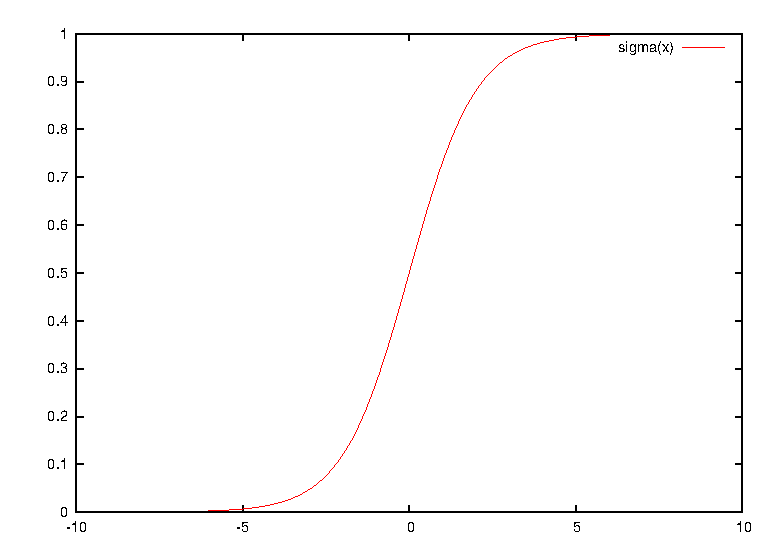
\includegraphics{sig}
\par\end{centering}
\caption{An example plot of the sigmoid function.\protect\label{fig:examplePlot}}

\end{figure}
As is evident from this particular form, this function tends very
quickly to 1 as $x$ goes to infinity and very quickly to 0 as the
parameter $x$ gets negative values. This phenomenon has the effect
of the artificial neuronal network to lose its general abilities,
as large changes in the values of the parameters cause no substantial
change in the response of the sigmoid function. The function $B(a)$
is used here to measure this effect and it is calculated using the
algorithm \ref{alg:CalculationBound}.

{\bfseries{}
\begin{algorithm}[H]
\textbf{\caption{Calculating the quantity $B(N\left(\protect\overrightarrow{x},\protect\overrightarrow{w}\right),a)$
with $a>0$ for a a provided neural network $N(x,w).$\protect\label{alg:CalculationBound}}
}
\begin{enumerate}
\item \textbf{Function} $B(N\left(\overrightarrow{x},\overrightarrow{w}\right),a)$
\item \textbf{Define $c=0$}
\item \textbf{For $i=1..H$ Do}
\begin{enumerate}
\item \textbf{For $j=1..M$ Do}
\begin{enumerate}
\item Set $v=\sum_{k=1}^{d}\left(w_{(d+2)i-(d+i)+k}x_{jk}\right)+w_{(d+2)i}$
\item \textbf{If $\left|v\right|>a$ then $c=c+1$}
\end{enumerate}
\item \textbf{EndFor}
\end{enumerate}
\item \textbf{EndFor}
\item \textbf{Return $\frac{c}{H\star M}$}
\item \textbf{End Function}
\end{enumerate}
\end{algorithm}
}The function $B(N\left(\overrightarrow{x},\overrightarrow{w}\right),a)$
is used to calculate the fitness value for the used genetic algorithm
described subsequently:
\begin{enumerate}
\item \textbf{Initialization step}.
\begin{enumerate}
\item \textbf{Set} the number of chromosomes denoted as $N_{c}$ and the
maximum number of allowed generations $N_{g}$.
\item \textbf{Set} as $p_{s}$ the selection rate and as $p_{m}$ the mutation
rate.
\item \textbf{Initialize} randomly the $N_{c}$ chromosomes. Each chromosome
$g_{i},\ i=1,..,N_{c}$ represents a neural network $N\left(\overrightarrow{x},\overrightarrow{g_{i}}\right)$.
\item \textbf{Set} $k=0$, the generation counter.
\end{enumerate}
\item \textbf{Fitness calculation step}.
\begin{enumerate}
\item \textbf{For} each chromosome $g_{i},\ i=1,..,N_{c}$ \textbf{do}
\begin{enumerate}
\item \textbf{Set} $E\left(N\left(\overrightarrow{x},\overrightarrow{g_{i}}\right)\right)=\sum_{j=1}^{M}\left(N\left(\overrightarrow{x_{j}},\overrightarrow{g_{i}}\right)-y_{j}\right)^{2}$
\item \textbf{Set} $b_{i}=B(N\left(\overrightarrow{x},\overrightarrow{g_{i}}\right),a)$
\item \textbf{Set} $f_{i}=E\left(N\left(\overrightarrow{x},\overrightarrow{g_{i}}\right)\right)\times\left(1+\lambda b_{i}^{2}\right)$
as the fitness value of chromosome $g_{i}$. The value $\lambda$
has the property $\lambda>1$.
\end{enumerate}
\item \textbf{End For}
\end{enumerate}
\item \textbf{Genetic operations step}.
\begin{enumerate}
\item \textbf{Copy} the best $\left(1-p_{s}\right)\times N_{c}$ chromosomes
to the next generation. The remaining will be substituted by individuals
produced by crossover and mutation.
\item \textbf{Perform }the crossover procedure. For every pair of constructed
chromosomes $\left(\widetilde{z},\widetilde{w}\right)$ two chromosomes
are selected from the current population using tournament selection.
The new chromosomes are created through the process suggested by Kaelo
et al \citep{kaelo}.
\item \textbf{Perform} the mutation procedure. For every element of each
chromosome alter this element randomly with probability $p_{m}$.
\end{enumerate}
\item \textbf{Termination check step}.
\begin{enumerate}
\item \textbf{Set} $k=k+1$
\item \textbf{If} $k<N_{g}$ \textbf{goto} fitness calculation step.
\end{enumerate}
\item \textbf{Bound creation step}.
\begin{enumerate}
\item \textbf{Obtain} the best chromosome $g^{*}$
\item \textbf{Create} the vectors $L^{*}$and $R^{*}$ as: 
\[
\begin{array}{ccc}
L_{i}^{*} & = & -f\left|g_{i}^{*}\right|,\ i=1,\ldots,n\\
R_{i}^{*} & = & f\left|g_{i}^{*}\right|,\ i=1,\ldots,n
\end{array}
\]
where $f>1$
\end{enumerate}
\end{enumerate}

\subsection{The bounding technique of the second phase }

During the second phase of the proposed algorithm, a systematic attempt
is made to identify the optimal value interval within the vectors
$L^{*}$ and $R^{*}$ identified in the previous phase. For this reason,
an evolutionary technique that has its bases in the differential evolution
technique is applied here. In this phase, the agents that constitute
the candidate solutions generated by the differential evolution technique
constitute ranges of values defined as: $\left[\overrightarrow{L_{k}},\overrightarrow{R_{k}}\right]$.
Also, the fitness value for each agent is defined as an interval $f=\left[f_{1},f_{2}\right].$
In order to compare two intervals $a=\left[a_{1},a_{2}\right]$ and
$b=\left[b_{1},b_{2}\right]$ the comparison operator $D(a,b)$ is
used with the following definition:
\begin{equation}
D(a,b)=\begin{cases}
\mbox{TRUE}, & a_{1}<b_{1},\mbox{OR\ \ensuremath{\left(a_{1}=b_{1}\ \mbox{AND}\ a_{2}<b_{2}\right)}}\\
\mbox{FALSE}, & \mbox{\mbox{OTHERWISE}}
\end{cases}\label{eq:eqD}
\end{equation}
The steps of the procedure used in the second phase have as follows:
\begin{enumerate}
\item \textbf{Initialization step}.
\begin{enumerate}
\item \textbf{Set} the number of agents NP.
\item \textbf{Set} the crossover probability CR.
\item \textbf{Set} the maximum number of iterations $N_{k}$.
\item \textbf{Set} the number of samples $N_{s}$.
\item \textbf{Initialize} each agent $a_{i}=$$\left[\overrightarrow{L_{i}},\overrightarrow{R_{i}}\right],\ i=1,\ldots,\mbox{NP}$
randomly inside the vectors $L^{*}$and $R^{*}$ of the previous phase.
\item \textbf{Set} $k=0$ as the iteration counter.
\end{enumerate}
\item \textbf{Fitness calculation step.}
\begin{enumerate}
\item \textbf{For} $i=1,\ldots,\mbox{NP}$ \textbf{do}
\begin{enumerate}
\item \textbf{Calculate} the fitness $f_{i}$ of agent $a_{i}$ using the
algorithm \ref{alg:fitnessCalculation}.
\end{enumerate}
\item \textbf{End} \textbf{For}
\end{enumerate}
\item \textbf{Main step}.
\begin{enumerate}
\item \textbf{For} $i=1,\ldots,\mbox{NP}$ \textbf{do}
\begin{enumerate}
\item \textbf{Select} randomly three distinct agents $a_{r1},a_{r2},a_{r3}$.
\item \textbf{Select} randomly an integer value $R\in[0,n].$
\item Set $t=a_{i}$ as the trial point .
\item \textbf{For} $j=1,\ldots,n$ \textbf{do}
\begin{enumerate}
\item \textbf{If} $j=R$ OR $r\le\mbox{CR}$ set $t_{j}=a_{r1,j}+F_{r}\times\left(a_{r2,j}-a_{r3,j}\right)$
where $r$ and $F_{r}$ are random values in {[}0,1{]}.
\end{enumerate}
\item \textbf{End For}
\item \textbf{Set} $t_{f}$ as the fitness of the trial set of intervals
$t$. This fitness value is calculated using the algorithm \ref{alg:fitnessCalculation}.
\item \textbf{If} $d\left(t_{f},f_{i}\right)=\mbox{TRUE}$ \textbf{then}
$a_{i}=t$.
\end{enumerate}
\item \textbf{End For}
\end{enumerate}
\item \textbf{Termination check step}.
\begin{enumerate}
\item \textbf{Set} $k=k+1$
\item \textbf{If} $k\le N_{k}$ goto Main Step.
\end{enumerate}
\item \textbf{Final step}.
\begin{enumerate}
\item \textbf{Obtain} the best agent $a^{*}=\left[\overrightarrow{L_{a}^{*}},\overrightarrow{R_{a}^{*}}\right]$
\item \textbf{Return} $a^{*}$ as the best located interval.
\end{enumerate}
%
\end{enumerate}
\begin{algorithm}[H]

\caption{Fitness calculation for any agent $a=\left[\protect\overrightarrow{L_{a}},\protect\overrightarrow{R_{a}}\right]$.\protect\label{alg:fitnessCalculation}}

\begin{enumerate}
\item \textbf{Take} $N_{s}$ random samples in $a$ and form the set $S_{a}=\left\{ \overrightarrow{s_{1}},\overrightarrow{s_{2},}\ldots,\overrightarrow{s_{N_{s}}}\right\} $.
\item \textbf{Set} $f_{\mbox{min}}=\infty$
\item \textbf{Set} $f_{\max}=-\infty$
\item \textbf{For} $i=1,\ldots,N_{s}$ \textbf{do}
\begin{enumerate}
\item \textbf{Calculate} $E_{i}=\sum_{j=1}^{M}\left(N\left(\overrightarrow{x_{j}},\overrightarrow{s_{i}}\right)-y_{j}\right)^{2}$
\item \textbf{If} $E_{i}<f_{\mbox{min}}$ set $f_{\mbox{min}}=E_{i}$
\item \textbf{If} $E_{i}>f_{\mbox{max}}$ set $f_{\mbox{max}}=E_{i}$
\end{enumerate}
\item \textbf{End For}
\item \textbf{Return} as fitness value the quantity $f_{a}=\left[f_{\mbox{min}},f_{\mbox{max}}\right]$
\end{enumerate}
\end{algorithm}


\subsection{The final training method}

In the last phase of the proposed procedure, a genetic algorithm is
applied to train the artificial neural network. The network is trained
within the interval $a^{*}$ identified in the second phase of the
procedure. The main steps of this genetic algorithm have as follows:
\begin{enumerate}
\item \textbf{Initialization step}.
\begin{enumerate}
\item \textbf{Set} as $N_{c}$ the number of chromosomes and as $N_{g}$
the maximum number of allowed generations.
\item \textbf{Set} as $p_{s}$ the selection rate and as $p_{m}$ the mutation
rate.
\item \textbf{Initialize} each chromosome $g_{i},\ i=1,\ldots,N_{c}$ inside
the bounds $a^{*}=\left[\overrightarrow{L_{a}^{*}},\overrightarrow{R_{a}^{*}}\right]$
of the second phase.
\item \textbf{Set} $k=0$ as the generation number.
\end{enumerate}
\item \textbf{Fitness calculation step}.
\begin{enumerate}
\item \textbf{For} $i=1,\ldots,N_{c}$ \textbf{do}
\begin{enumerate}
\item \textbf{Obtain} the neural network $N_{i}=N\left(\overrightarrow{x},\overrightarrow{g_{i}}\right)$
for each chromosome $\overrightarrow{g_{i}}$.
\item \textbf{Set} $f_{i}=\sum_{j=1}^{M}\left(N\left(\overrightarrow{x_{j}},\overrightarrow{g_{i}}\right)-y_{j}\right)^{2}$
as the associated fitness value.
\end{enumerate}
\item \textbf{End For}
\end{enumerate}
\item \textbf{Genetic operations step}.
\begin{enumerate}
\item \textbf{Perform} selection, crossover and mutation using the same
operations as in the first phase of the proposed method.
\end{enumerate}
\item \textbf{Termination check step}.
\begin{enumerate}
\item \textbf{Set} $k=k+1$
\item \textbf{If} $k\le N_{g}$ goto Fitness Calculation Step.
\end{enumerate}
\item \textbf{Testing step}.
\begin{enumerate}
\item \textbf{Obtain} the best chromosome $\overrightarrow{g^{*}}$. 
\item \textbf{Create} the corresponding neural network $N\left(\overrightarrow{x},\overrightarrow{g^{*}}\right)$
\item \textbf{Apply} this neural network to the associated test set and
report the results.
\end{enumerate}
\end{enumerate}
%
The overall procedure is graphically outlined in the flowchart of
Figure \ref{fig:flow}.

\begin{figure}[H]
\begin{centering}
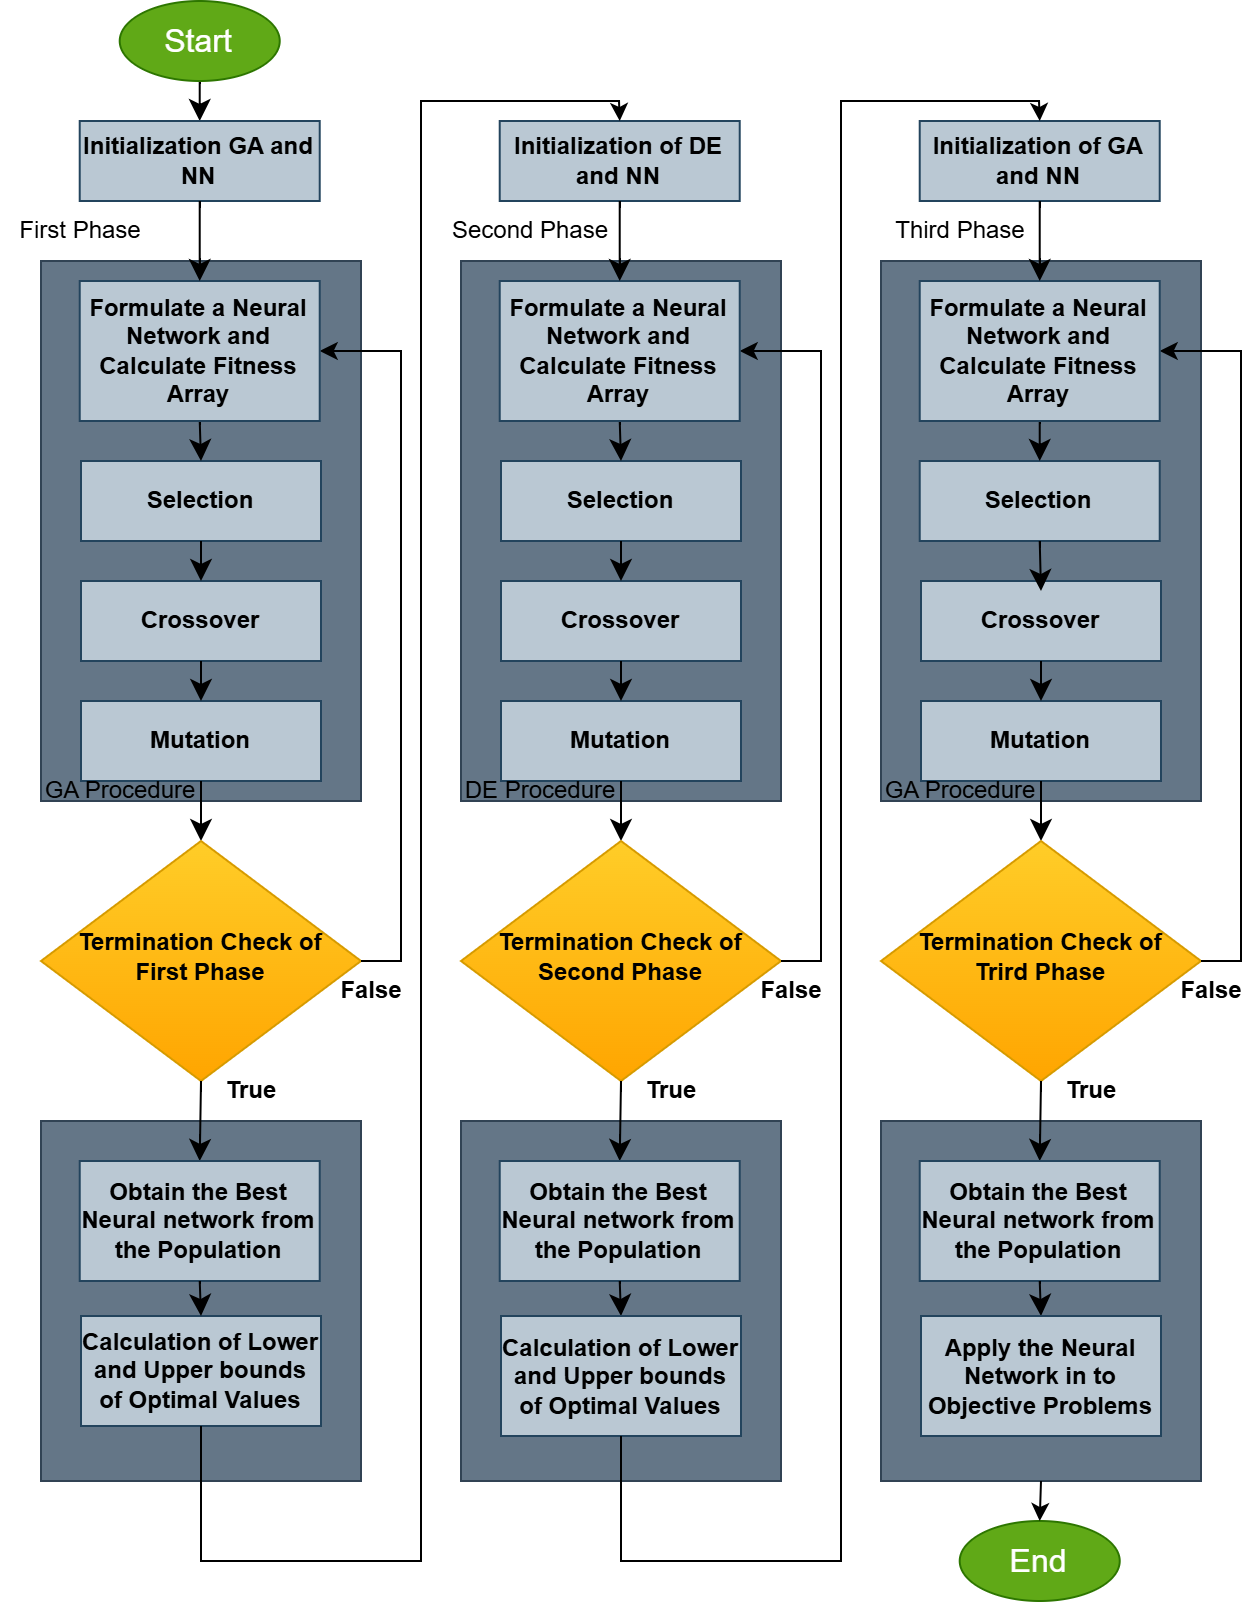
\includegraphics[scale=0.5]{flowChart}
\par\end{centering}
\caption{The flowchart of the proposed algorithm.\protect\label{fig:flow}}

\end{figure}


\subsection{The used datasets}

The proposed method was tested for its efficiency on a series of classification
and regression problems, that were obtained from the following online
databases:
\begin{enumerate}
\item The UCI database located in \url{https://archive.ics.uci.edu/}(accessed
on 17 February 2025)\citep{uci}
\item The Keel website, \url{https://sci2s.ugr.es/keel/datasets.php}(accessed
on 17 February 2025)\citep{Keel}.
\item The Statlib URL \url{ftp://lib.stat.cmu.edu/datasets/index.html }(accessed
on 17 February 2025). 
\end{enumerate}
The following series of classification datasets was used in the conducted
experiments:
\begin{enumerate}
\item \textbf{Appendicitis}, which is medical dataset proposed in \citep{appendicitis}. 
\item \textbf{Alcohol}, which is related to experiments regarding alcohol
consumption \citep{alcohol}. 
\item \textbf{Australian}, which is related to various bank transactions\citep{australian}.
\item \textbf{Balance} dataset \citep{balance}, which is used in various
psychological experiments.
\item \textbf{Cleveland}, which is a medical dataset \citep{cleveland1}. 
\item \textbf{Circular} dataset, which is a dataset created artificially. 
\item \textbf{Dermatology}, a medical dataset with 6 classes which is related
to dermatology problems \citep{dermatology}.
\item \textbf{Ecoli}, which is used to problems regarding proteins \citep{ecoli}.
\item \textbf{Glass} dataset, which is related to glass component analysis. 
\item \textbf{Haberman}, a medical dataset for the detection of breast cancer. 
\item \textbf{Hayes-roth} dataset \citep{hayes-roth}, a dataset with 3
classes.
\item \textbf{Heart}, a medical dataset about heart diseases \citep{heart}
with two classes.
\item \textbf{HeartAttack}, a medical dataset used for the detection of
heart diseases.
\item \textbf{Housevotes}, that contains data about the Congressional voting
in USA \citep{housevotes}.
\item \textbf{Ionosphere}, that contains measurements about the ionosphere
\citep{ion1}.
\item \textbf{Liverdisorder}, which is a medical dataset \citep{liver}.
\item \textbf{Lymography }dataset \citep{lymography}.
\item \textbf{Mammographic}, a medical dataset related to breast cancer
\citep{mammographic}.
\item \textbf{Parkinsons}, a medical dataset related to Parkinson's disease
\citep{parkinsons1}.
\item \textbf{Pima}, a medical dataset related to the presence of diabetes\citep{pima}.
\item \textbf{Phoneme}, used in sound experiments.
\item \textbf{Popfailures}, a dataset that containsclimate measurements
\citep{popfailures}.
\item \textbf{Regions2}, a medical dataset related to some liver biopsy
images \citep{regions2}.
\item \textbf{Saheart}, which is a medical dataset related to some heart
diseases.\citep{saheart}.
\item \textbf{Segment} dataset \citep{segment}, used in various image processing
cases.
\item \textbf{Statheart}, which is a medical dataset related to heart diseases.
\item \textbf{Spiral}, which is a dataset created artificially. 
\item \textbf{Student}, a dataset that contains measurements from experiments
conducted in schools \citep{student}.
\item \textbf{Transfusion}, which is a medical dataset \citep{transfusion}.
\item \textbf{Wdbc}, a medical dataset used to predict the presence of breast
cancer \citep{wdbc1}.
\item \textbf{Wine}, a dataset used to predict the quality of wines \citep{wine1}.
\item \textbf{EEG} dataset, which is a medical dataset related to EEG measurements\citep{eeg1}
and the following cases were studied from this dataset: Z\_F\_S, ZO\_NF\_S
and ZONF\_S.
\item \textbf{Zoo}, a dataset used to predict the class of some animals
\citep{zoo} .
\end{enumerate}
Furthermore, the following list of regression datasets was incorporated
in the conducted experiments:
\begin{enumerate}
\item \textbf{Abalone}, a dataset related to the estimation of the age of
abalones \citep{abalone}.
\item \textbf{Airfoil}, a dataset provided by NASA \citep{airfoil}.
\item \textbf{Auto}, a dataset used for the estimation of fuel consumption
in cars.
\item \textbf{BK}, which is used in basketball games. 
\item \textbf{BL}, a dataset that contains measurements about electricity
experiments.
\item \textbf{Baseball}, a dataset that contains data used in the estimation
of the income of baseball players.
\item \textbf{Concrete}, a dataset used in civil engineering \citep{concrete}.
\item \textbf{DEE}, a dataset that contains 6 features, which is used for
the prediction of electricity prices.
\item \textbf{Friedman}, an artificial dataset\citep{friedman}.
\item \textbf{FY, }this dataset used to estimate the longevity of fruit
flies. 
\item \textbf{HO}, a dataset provided by the STATLIB repository with 13
features.
\item \textbf{Housing}, which is used for the prediction of house prices
\citep{housing}.
\item \textbf{Laser}, which is used in various laser experiments.
\item \textbf{LW}, which is a dataset with 9 features used to measure the
weight of babes.
\item \textbf{Mortgage}, which is a dataset with 15 features related to
the economy of USA.
\item \textbf{Plastic}, a dataset related to the pressure in plastics.
\item \textbf{PL}, a dataset provided by the STATLIB repository.
\item \textbf{Quake}, a dataset with 3 features that contains measurements
from earthquakes.
\item \textbf{SN}, a dataset with 11 features, which is used in experiments
related to trellising and pruning,.
\item \textbf{Stock}, a dataset with 9 features used to predict the prices
of various stocks.
\item \textbf{Treasury}, which is a dataset with 15 features used in economic
problems.
\end{enumerate}

\section{Results\protect\label{sec:Results}}

\subsection{Experimental results}

The software used in the conducted experiments was coded in C++, using
the freely available Optimus programming tool, that can be downloaded
from \url{https://github.com/itsoulos/GlobalOptimus/}( accessed on
17 February 2025 ). Each experiment was conducted 30 times using different
seed for the random generator each time. For the validation of the
experimental results the ten - fold cross validation method was used.
The average classification error as measured on the corresponding
test set is reported for the classification datasets. This error is
calculated using the following formula:
\begin{equation}
E_{C}\left(N\left(\overrightarrow{x},\overrightarrow{w}\right)\right)=100\times\frac{\sum_{i=1}^{N}\left(\mbox{class}\left(N\left(\overrightarrow{x_{i}},\overrightarrow{w}\right)\right)-y_{i}\right)}{N}
\end{equation}
In this formula the function $\mbox{class}\left(N\left(\overrightarrow{x_{i}},\overrightarrow{w}\right)\right)$
is used for the class obtained by the application of the neural network
to pattern $\overrightarrow{x_{i}}$. The sum of the differences of
the categories that the artificial neural network finds from the expected
categories is divided by the number of patterns in the dataset. Also,
the\textbf{ }average regression error is reported for the regression
datasets, that can be calculated as follows:
\begin{equation}
E_{R}\left(N\left(\overrightarrow{x},\overrightarrow{w}\right)\right)=\frac{\sum_{i=1}^{N}\left(N\left(\overrightarrow{x_{i}},\overrightarrow{w}\right)-y_{i}\right)^{2}}{N}
\end{equation}
In this formula the squared sum of the differences from the values
produced by the neural networks with the expected outputs is divided
by the sum of patterns in the dataset. All the experiments were performed
on\textbf{ }an AMD Ryzen 5950X with 128GB of RAM and the used operating
system was Debian Linux. The values used for the parameters of the
proposed method are shown in Table \ref{tab:settings}. 

\begin{table}[H]
\caption{The experimental settings used in the current algorithm.\protect\label{tab:settings}}

\centering{}%
\begin{tabular}{|c|c|c|}
\hline 
PARAMETER & MEANING & VALUE\tabularnewline
\hline 
\hline 
$H$ & Processing nodes & 10\tabularnewline
\hline 
$N_{c}$ & Chromosomes & 500\tabularnewline
\hline 
$N_{g}$ & Generations & 200\tabularnewline
\hline 
$p_{s}$ & Selection rate & 0.9\tabularnewline
\hline 
$p_{m}$ & Mutation rate & 0.05\tabularnewline
\hline 
$f$ & Bounding value & 2.0\tabularnewline
\hline 
$\mbox{NP}$ & Agents & 200\tabularnewline
\hline 
$F$ & Differential weight & 0.8\tabularnewline
\hline 
$\mbox{CR}$ & Crossover probability & 0.9\tabularnewline
\hline 
$N_{s}$ & Number of samples & 50\tabularnewline
\hline 
$N_{k}$ & Iterations & 200\tabularnewline
\hline 
\end{tabular}
\end{table}
The following notation is used in the tables that contains the measurement
from the conducted experiments:
\begin{enumerate}
\item The column DATASET contains the name of the used dataset.
\item The column ADAM represents the experimental results from the application
of the ADAM optimization method \citep{nn_adam} to a neural networks
with $H=10$ processing nodes. The Adam optimizer is a combination
of Momentum \citep{momentum} and RMSprop \citep{rmsprop} techniques
and it has been used successfully for neural network training in many
research papers.
\item The column BFGS denotes the incorporation of the BFGS optimization
method \citep{powell} to train an artificial neural network with
$H=10$ processing nodes. The Broyden--Fletcher--Goldfarb--Shanno
(BFGS) algorithm is a local optimization procedure that aims to discover
a local minima of a multidimensional function.
\item The column GENETIC represents the usage of a Genetic Algorithm with
the experimental settings of Table \ref{tab:settings}, used to train
a neural network with $H=10$ processing nodes.
\item The column RBF denotes the incorporation of a Radial Basis Function
(RBF) network \citep{rbf1} with $H=10$ processing nodes on the corresponding
dataset.
\item The column PRUNE represents the usage of OBS pruning method \citep{prune},
as implemented in the library Fast Compressed Neural Networks \citep{fcn}.
\item The column PROPOSED denotes the proposed method.
\item The row AVERAGE is used to measure the average classification or regression
error for all dataset.
\item The bold notation is used to indicate the method with the lowest classification
or regression error.
\end{enumerate}
The table \ref{tab:experClass} is used to provide the experimental
results for the classification datasets and the table \ref{tab:experRegression}
provides the corresponding results for the regression datasets.
\begin{table}[H]
\caption{Experimental results for the used classification datasets. The numbers
in cells represent average classification error as measured on the
corresponding test set.\protect\label{tab:experClass}}

\centering{}%
\begin{tabular}{|c|c|c|c|c|c|c|}
\hline 
DATASET & ADAM & BFGS & GENETIC & RBF & PRUNE & PROPOSED\tabularnewline
\hline 
\hline 
APPENDICITIS & 16.50\% & 18.00\% & 24.40\% & \textbf{12.23\%} & 15.97\% & 15.00\%\tabularnewline
\hline 
ALCOHOL & 57.78\% & 41.50\% & 39.57\% & 49.32\% & \textbf{15.75\%} & 18.33\%\tabularnewline
\hline 
AUSTRALIAN & 35.65\% & 38.13\% & 32.21\% & 34.89\% & 43.66\% & \textbf{21.49\%}\tabularnewline
\hline 
BALANCE & 12.27\% & 8.64\% & 8.97\% & 33.53\% & 9.00\% & \textbf{7.79\%}\tabularnewline
\hline 
CLEVELAND & 67.55\% & 77.55\% & 51.60\% & 67.10\% & 51.48\% & \textbf{42.38\%}\tabularnewline
\hline 
CIRCULAR & 19.95\% & 6.08\% & 5.99\% & \textbf{5.98\%} & 12.76\% & 6.50\%\tabularnewline
\hline 
DERMATOLOGY & 26.14\% & 52.92\% & 30.58\% & 62.34\% & 9.02\% & \textbf{4.97\%}\tabularnewline
\hline 
ECOLI & 64.43\% & 69.52\% & 54.67\% & 59.48\% & 60.32\% & \textbf{40.30\%}\tabularnewline
\hline 
GLASS & 61.38\% & 54.67\% & 52.86\% & \textbf{50.46\%} & 66.19\% & 54.38\%\tabularnewline
\hline 
HABERMAN & 29.00\% & 29.34\% & 28.66\% & \textbf{25.10\%} & 29.38\% & 26.53\%\tabularnewline
\hline 
HAYES-ROTH & 59.70\% & 37.33\% & 56.18\% & 64.36\% & 45.44\% & \textbf{34.31\%}\tabularnewline
\hline 
HEART & 38.53\% & 39.44\% & 28.34\% & 31.20\% & 27.21\% & \textbf{13.11\%}\tabularnewline
\hline 
HEARTATTACK & 45.55\% & 46.67\% & 29.03\% & 29.00\% & 29.26\% & \textbf{21.90\%}\tabularnewline
\hline 
HOUSEVOTES & 7.48\% & 7.13\% & 6.62\% & 6.13\% & \textbf{5.81\%} & 6.09\%\tabularnewline
\hline 
IONOSPHERE & 16.64\% & 15.29\% & 15.14\% & 16.22\% & 11.32\% & \textbf{10.37\%}\tabularnewline
\hline 
LIVERDISORDER & 41.53\% & 42.59\% & 31.11\% & 30.84\% & 49.72\% & \textbf{29.94\%}\tabularnewline
\hline 
LYMOGRAPHY & 39.79\% & 35.43\% & 28.42\% & 25.50\% & 22.02\% & \textbf{17.93\%}\tabularnewline
\hline 
MAMMOGRAPHIC & 46.25\% & 17.24\% & 19.88\% & 21.38\% & 38.10\% & \textbf{16.63\%}\tabularnewline
\hline 
PARKINSONS & 24.06\% & 27.58\% & 18.05\% & 17.41\% & 22.12\% & \textbf{12.79\%}\tabularnewline
\hline 
PHONEME & 29.43\% & 15.58\% & \textbf{15.55\%} & 23.32\% & 29.35\% & 18.10\%\tabularnewline
\hline 
PIMA & 34.85\% & 35.59\% & 32.19\% & 25.78\% & 35.08\% & \textbf{25.03\%}\tabularnewline
\hline 
POPFAILURES & 5.18\% & 5.24\% & 5.94\% & 7.04\% & 4.79\% & \textbf{4.45\%}\tabularnewline
\hline 
REGIONS2 & 29.85\% & 36.28\% & 29.39\% & 38.29\% & 34.26\% & \textbf{25.19\%}\tabularnewline
\hline 
SAHEART & 34.04\% & 37.48\% & 34.86\% & 32.19\% & 37.70\% & \textbf{29.26\%}\tabularnewline
\hline 
SEGMENT & 49.75\% & 68.97\% & 57.72\% & 59.68\% & 60.40\% & \textbf{27.80\%}\tabularnewline
\hline 
SONAR & 30.33\% & 25.85\% & 22.40\% & 27.90\% & 23.80\% & \textbf{20.50\%}\tabularnewline
\hline 
SPIRAL & 47.67\% & 47.99\% & 48.66\% & 44.87\% & 50.38\% & \textbf{41.60\%}\tabularnewline
\hline 
STATHEART & 44.04\% & 39.65\% & 27.25\% & 31.36\% & 28.37\% & \textbf{19.74\%}\tabularnewline
\hline 
STUDENT & 5.13\% & 7.14\% & 5.61\% & 5.49\% & 10.84\% & \textbf{4.00\%}\tabularnewline
\hline 
TRANSFUSION & 25.68\% & 25.84\% & 24.87\% & 26.41\% & 29.35\% & \textbf{23.35\%}\tabularnewline
\hline 
WDBC & 35.35\% & 29.91\% & 8.56\% & 7.27\% & 15.48\% & \textbf{6.73\%}\tabularnewline
\hline 
WINE & 29.40\% & 59.71\% & 19.20\% & 31.41\% & 16.62\% & \textbf{6.29\%}\tabularnewline
\hline 
Z\_F\_S & 47.81\% & 39.37\% & 10.73\% & 13.16\% & 17.91\% & \textbf{8.38\%}\tabularnewline
\hline 
ZO\_NF\_S & 47.43\% & 43.04\% & 21.54\% & 9.02\% & 15.57\% & \textbf{4.32\%}\tabularnewline
\hline 
ZONF\_S & 11.99\% & 15.62\% & 4.36\% & 4.03\% & 3.27\% & \textbf{1.76\%}\tabularnewline
\hline 
ZOO & 14.13\% & 10.70\% & 9.50\% & 21.93\% & 8.53\% & \textbf{7.00\%}\tabularnewline
\hline 
\textbf{AVERAGE} & \textbf{34.23\%} & \textbf{33.58\%} & \textbf{26.13\%} & \textbf{29.21\%} & \textbf{27.40\%} & \textbf{18.73\%}\tabularnewline
\hline 
\end{tabular}
\end{table}
\begin{table}[H]
\caption{Experimental results for the used regression datasets. Numbers in
cells represent average regression error as calculated on the corresponding
test set.\protect\label{tab:experRegression}}

\centering{}%
\begin{tabular}{|c|c|c|c|c|c|c|}
\hline 
DATASET & ADAM & BFGS & GENETIC & RBF & PRUNE & PROPOSED\tabularnewline
\hline 
\hline 
ABALONE & 4.30 & 5.69 & 7.17 & 7.37 & 7.88 & \textbf{4.32}\tabularnewline
\hline 
AIRFOIL & 0.005 & 0.003 & 0.003 & 0.27 & 0.002 & \textbf{0.002}\tabularnewline
\hline 
AUTO & 70.84 & 60.97 & \textbf{12.18} & 17.87 & 75.59 & 12.78\tabularnewline
\hline 
BK & 0.0252 & 0.28 & 0.027 & 0.02 & 0.027 & \textbf{0.02}\tabularnewline
\hline 
BL & 0.622 & 2.55 & 5.74 & 0.013 & 0.027 & \textbf{0.006}\tabularnewline
\hline 
BASEBALL & 77.90 & 119.63 & 103.60 & 93.02 & 94.50 & \textbf{60.74}\tabularnewline
\hline 
CONCRETE & 0.078 & 0.066 & 0.0099 & 0.011 & 0.0077 & \textbf{0.006}\tabularnewline
\hline 
DEE & 0.63 & 2.36 & 1.013 & \textbf{0.17} & 1.08 & 0.19\tabularnewline
\hline 
FRIEDMAN & 22.90 & 1.263 & \textbf{1.249} & 7.23 & 8.69 & 2.21\tabularnewline
\hline 
FY & \textbf{0.038} & 0.19 & 0.65 & 0.041 & 0.042 & 0.067\tabularnewline
\hline 
HO & 0.035 & 0.62 & 2.78 & 0.03 & 0.03 & \textbf{0.015}\tabularnewline
\hline 
HOUSING & 80.99 & 97.38 & 43.26 & 57.68 & 52.25 & \textbf{20.74}\tabularnewline
\hline 
LASER & 0.03 & 0.015 & 0.59 & 0.03 & 0.007 & \textbf{0.004}\tabularnewline
\hline 
LW & 0.028 & 2.98 & 1.90 & 0.03 & 0.02 & \textbf{0.011}\tabularnewline
\hline 
MORTGAGE & 9.24 & 8.23 & 2.41 & 1.45 & 12.96 & \textbf{0.32}\tabularnewline
\hline 
PL & 0.117 & 0.29 & 0.29 & 2.118 & 0.032 & \textbf{0.022}\tabularnewline
\hline 
PLASTIC & 11.71 & 20.32 & 2.791 & 8.62 & 17.33 & \textbf{2.16}\tabularnewline
\hline 
QUAKE & 0.07 & 0.42 & 0.04 & 0.07 & 0.04 & \textbf{0.036}\tabularnewline
\hline 
SN & 0.026 & 0.40 & 2.95 & 0.027 & 0.032 & \textbf{0.023}\tabularnewline
\hline 
STOCK & 180.89 & 302.43 & \textbf{3.88} & 12.23 & 39.08 & 5.57\tabularnewline
\hline 
TREASURY & 11.16 & 9.91 & 2.93 & 2.02 & 13.76 & \textbf{0.68}\tabularnewline
\hline 
\textbf{AVERAGE} & \textbf{22.46} & \textbf{30.29} & \textbf{9.31} & \textbf{10.02} & \textbf{15.40} & \textbf{5.23}\tabularnewline
\hline 
\end{tabular}
\end{table}

The Table \ref{tab:experClass} presents a detailed comparison of
the performance of six different machine learning models, namely ADAM,
BFGS, GENETIC, RBF, PRUNE, and PROPOSED, evaluated across multiple
classification datasets. The values in the table represent the error
rates for each model on each dataset, expressed as percentages. Lower
error rates indicate better performance for a given model on a specific
dataset. The last row of the table provides the average error rate
for each model, serving as a measure of their overall effectiveness
across all datasets. From the analysis of this table, it becomes evident
that the PROPOSED model achieves the best overall performance, with
an average error rate of 18.73\%. This is the lowest among all the
models evaluated, demonstrating its superior effectiveness in solving
classification problems across a diverse set of datasets. In particular,
the PROPOSED model consistently outperforms the other models in datasets
such as DERMATOLOGY, ZONF\_S, and ZOO, where it records the smallest
error rates, indicating its robustness in handling datasets of varying
complexity and characteristics. The GENETIC model, on the other hand,
has the highest average error rate at 26.13\%, making it the least
effective model overall. This result suggests that while the GENETIC
model may perform adequately in certain contexts, it lacks the adaptability
and overall reliability exhibited by the PROPOSED model. Examining
the ADAM model, we observe an average error rate of 34.23\%, which
is one of the highest among the models. Despite this, ADAM demonstrates
good performance in specific datasets, such as CIRCULAR and SPIRAL,
where its error rates are notably low. This indicates that the performance
of ADAM is heavily dependent on the structure and features of the
datasets, performing well in certain contexts but underperforming
in others. Similarly, the BFGS model has an average error rate of
33.58\%, slightly lower than ADAM, but it exhibits comparable variability
in its performance across datasets. The RBF model, with an average
error rate of 29.21\%, performs better than both ADAM and BFGS. RBF
appears to be more stable in its performance, achieving lower error
rates across a broader range of datasets, although it does not consistently
outperform the PROPOSED model. The PRUNE model achieves an average
error rate of 27.40\%, which places it between RBF and GENETIC in
terms of overall effectiveness. While PRUNE does not outperform the
PROPOSED model in most cases, it shows competitive performance in
datasets such as GLASS, where it records one of the lowest error rates.
This highlights that PRUNE can be effective in certain specialized
datasets, though it lacks the overall adaptability of the PROPOSED
model. A closer inspection of specific datasets further reinforces
the dominance of the PROPOSED model. For instance, in the STATHEART
and WINE datasets, which are characterized by increased complexity,
the PROPOSED model achieves significantly lower error rates compared
to the other models, indicating its ability to handle challenging
classification tasks effectively. Additionally, in the HOUSEVOTES
dataset, the PROPOSED model performs exceptionally well, suggesting
its reliability in datasets with distinct structures. The GENETIC
model, while generally less effective, demonstrates relatively strong
performance in a few datasets such as HAYES-ROTH and SPIRAL, where
its error rates are comparable to or better than those of other models.
However, its overall high average error rate indicates that its performance
is inconsistent and heavily dependent on the specific dataset. Similarly,
PRUNE performs well in datasets like MAMMOGRAPHIC but falls behind
in others, such as SEGMENT and BALANCE, where the PROPOSED model outperforms
it by a considerable margin. The results for the BFGS model reveal
a mixed performance profile. It achieves relatively low error rates
in datasets such as BALANCE and HEART, but it struggles in datasets
like CLEVELAND and LIVERDISORDER, where its error rates are higher
than most of the other models. This inconsistency highlights the model’s
limited generalizability across datasets. In conclusion, the PROPOSED
model demonstrates the best overall performance across the majority
of the datasets, achieving the lowest average error rate and consistently
outperforming the other models in a wide range of contexts. This suggests
that the PROPOSED model is highly adaptable and effective, making
it suitable for diverse classification tasks. The analysis further
underscores the importance of selecting the appropriate model based
on the characteristics of the dataset, as models like ADAM, BFGS,
and PRUNE show strong performance in specific scenarios but fall short
in others. The average error rate remains a critical indicator for
evaluating the overall effectiveness of the models, providing valuable
insights into their strengths and weaknesses.

The dynamics of the proposed technique on the classification data
is also presented graphically in Figure \ref{fig:The-average-classification},
where the average classification error per method is presented.
\begin{figure}[H]
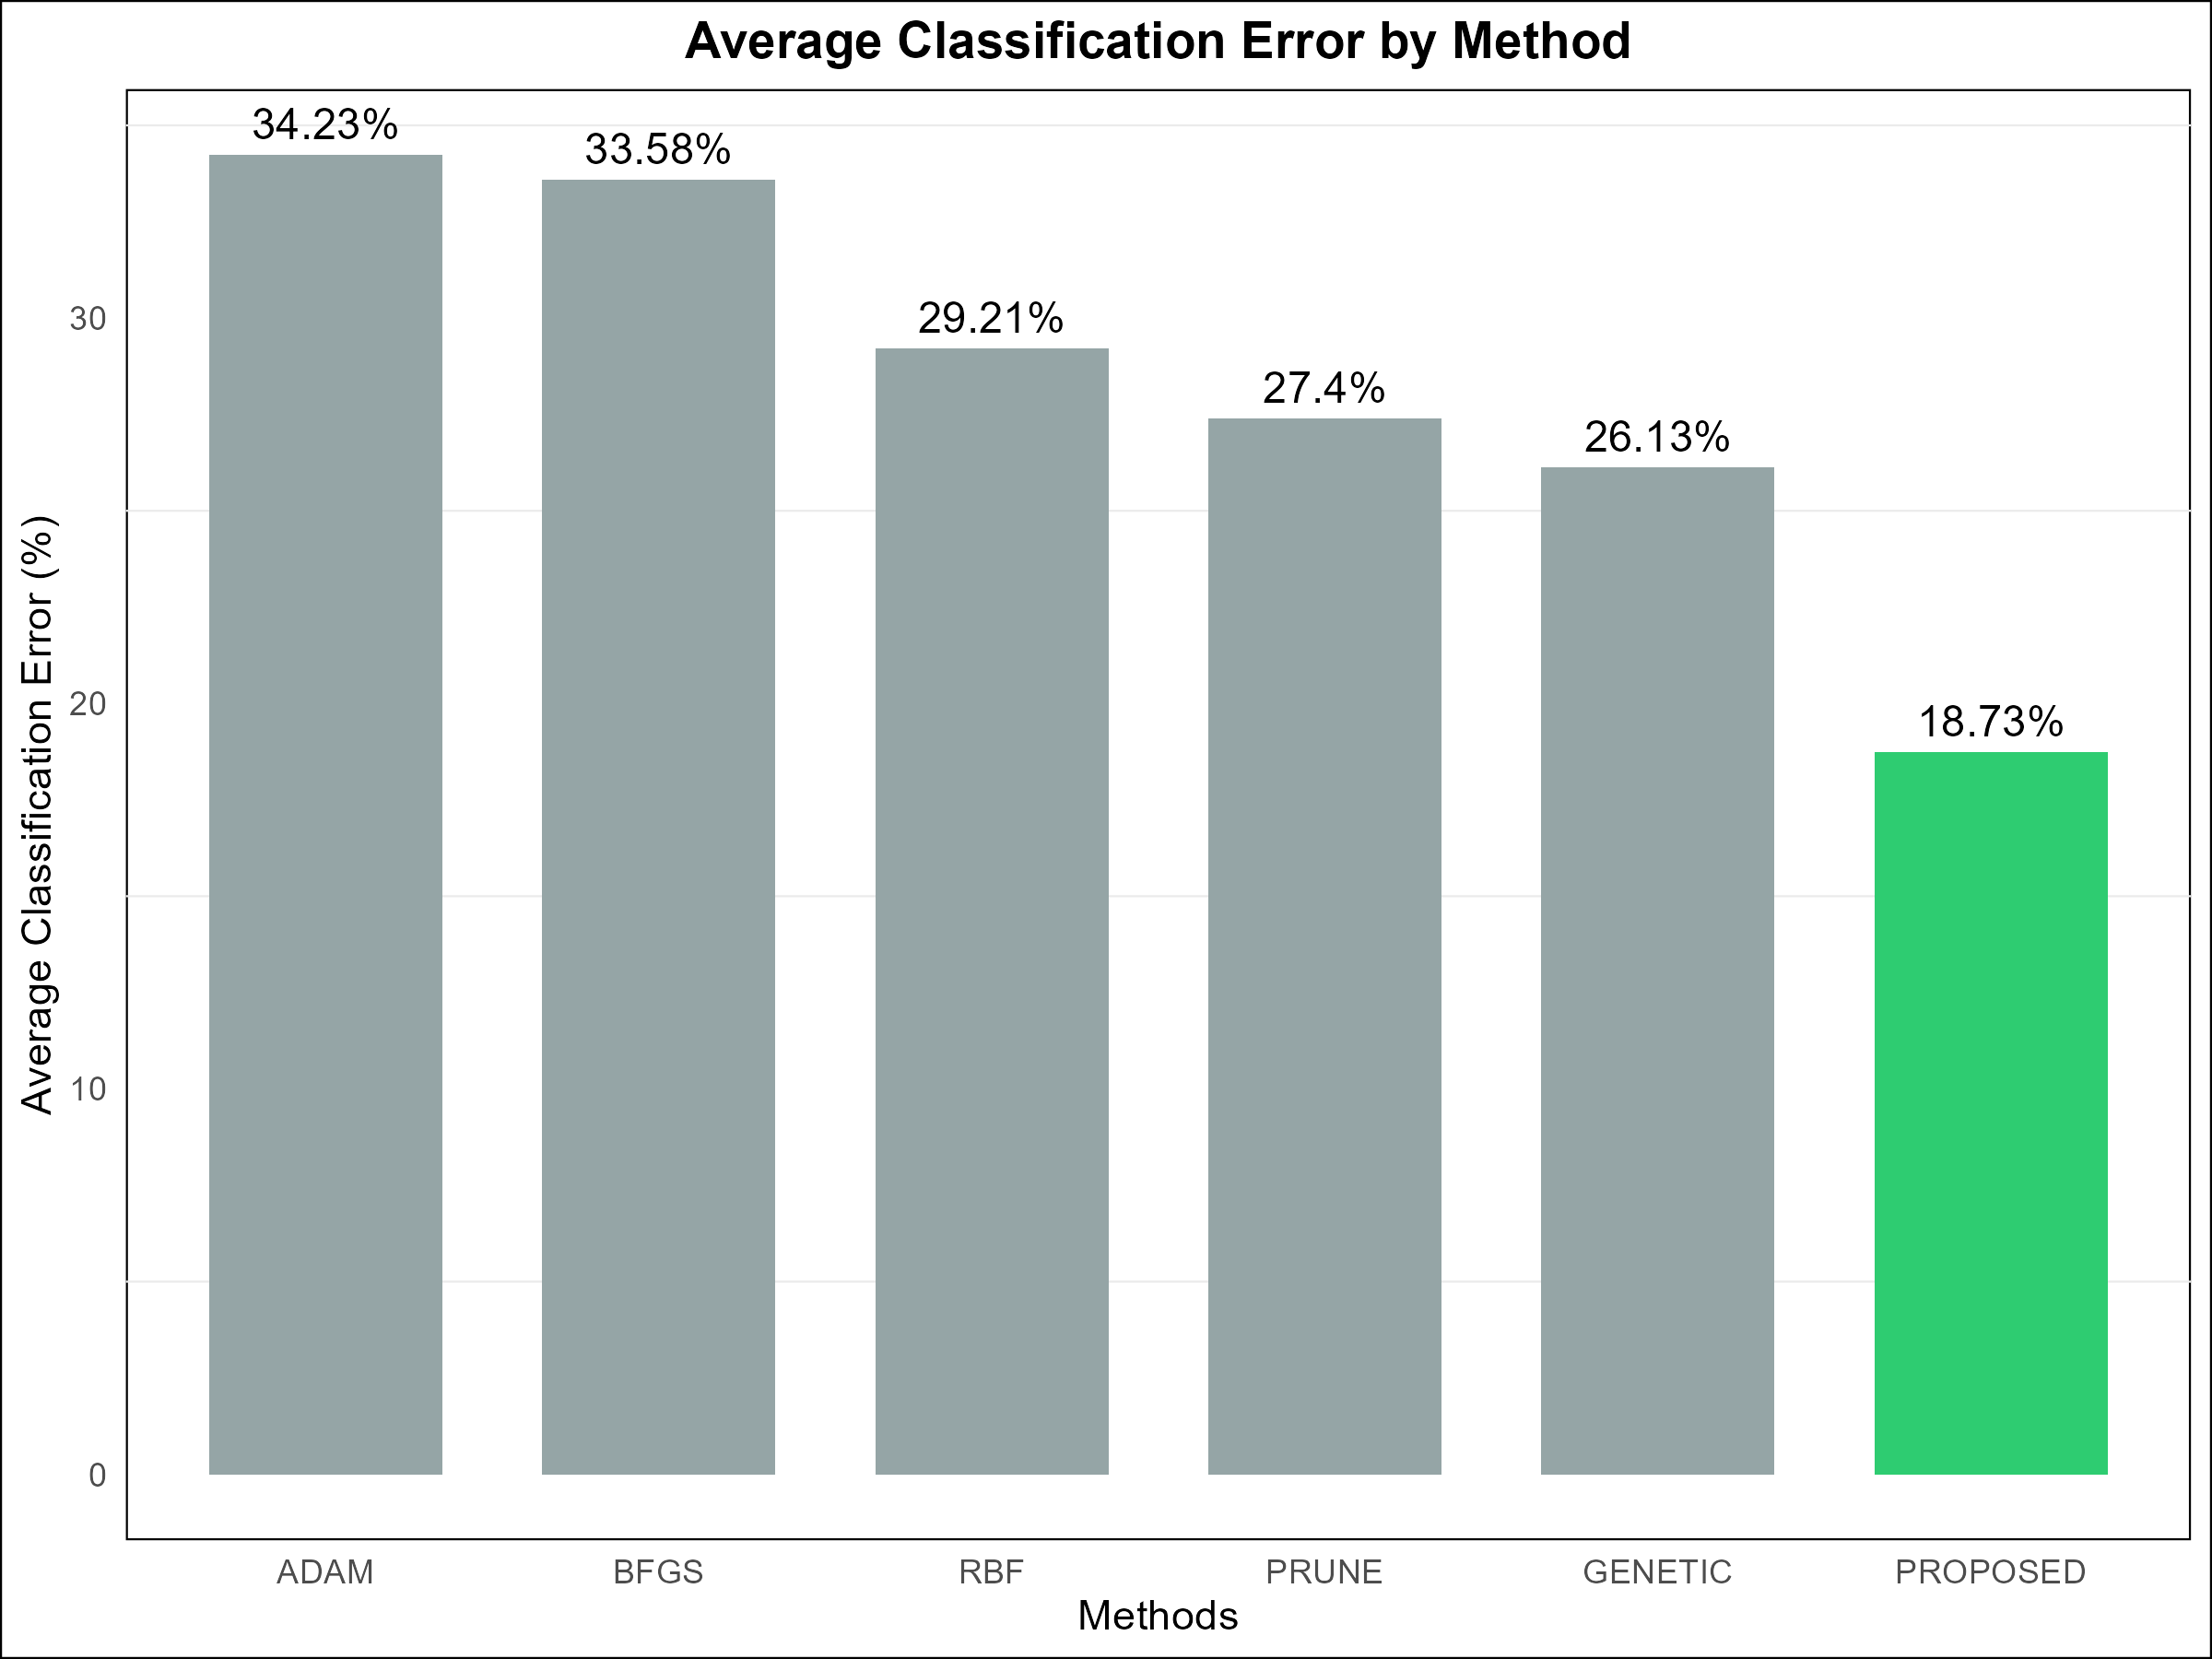
\includegraphics[scale=0.5]{average_barchart}

\caption{The average classification error for all methods used in the conducted
experiments.\protect\label{fig:The-average-classification}}

\end{figure}
 Furthermore, Figure \ref{fig:casesReduction} graphically presents
the number of cases in which there was a significant reduction in
classification error between the simple genetic algorithm and the
proposed method. As is evident, in a significant number of cases there
is a drastic reduction in classification error exceeding 20\% \LyXZeroWidthSpace\LyXZeroWidthSpace or
even 40\%.
\begin{figure}[H]
\begin{centering}
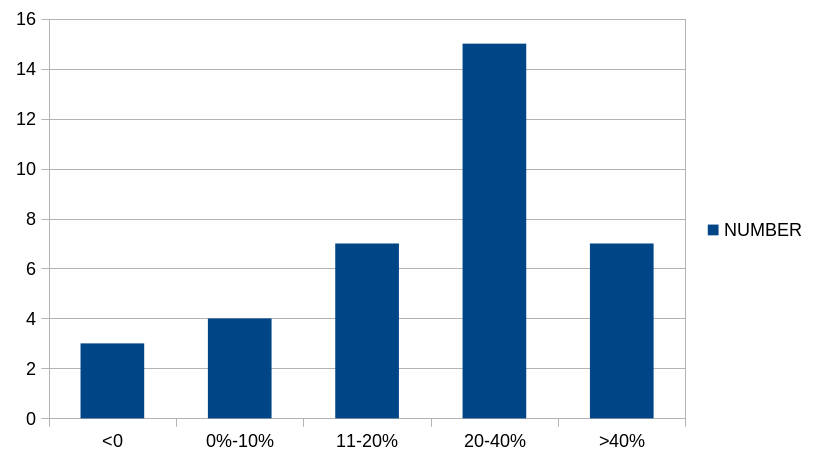
\includegraphics[scale=0.75]{class_improve}
\par\end{centering}
\caption{Number of cases for the classification datasets where a reduction
was appeared in the classification error between the original genetic
algorithm and the proposed method.\protect\label{fig:casesReduction}}

\end{figure}
. Also, a comparison for the factors of precision and recall between
the original genetic algorithm and the proposed method is outlined
in Table \ref{tab:precisionAndRecall} for the classification datasets.

\begin{table}[H]
\caption{Comparison of precision and recall between the original genetic algorithm
and the proposed method.\protect\label{tab:precisionAndRecall}}

\centering{}%
\begin{tabular}{|c|c|c|c|c|}
\hline 
 & \multicolumn{2}{c|}{GENETIC} & \multicolumn{2}{c|}{\textbf{PROPOSED}}\tabularnewline
\hline 
\hline 
\textbf{DATASET} & \textbf{PRECISION} & \textbf{RECALL} & \textbf{PRECISION} & \textbf{RECALL}\tabularnewline
\hline 
APPENDICITIS & 0.81 & 0.81 & 0.86 & 0.85\tabularnewline
\hline 
ALCOHOL & 0.58 & 0.61 & 0.83 & 0.83\tabularnewline
\hline 
AUSTRALIAN & 0.67 & 0.66 & 0.79 & 0.80\tabularnewline
\hline 
BALANCE & 0.83 & 0.88 & 0.86 & 0.92\tabularnewline
\hline 
CLEVELAND & 0.43 & 0.53 & 0.45 & 0.59\tabularnewline
\hline 
CIRCULAR & 0.91 & 0.91 & 0.94 & 0.94\tabularnewline
\hline 
DERMATOLOGY & 0.72 & 0.90 & 0.90 & 0.88\tabularnewline
\hline 
ECOLI & 0.41 & 0.44 & 0.54 & 0.59\tabularnewline
\hline 
GLASS & 0.47 & 0.58 & 0.48 & 0.52\tabularnewline
\hline 
HABERMAN & 0.61 & 0.59 & 0.62 & 0.61\tabularnewline
\hline 
HAYES ROTH & 0.40 & 0.47 & 0.70 & 0.65\tabularnewline
\hline 
HEART & 0.70 & 0.69 & 0.86 & 0.85\tabularnewline
\hline 
HEARTATTACK & 0.71 & 0.70 & 0.77 & 0.78\tabularnewline
\hline 
HOUSEVOTES & 0.91 & 0.92 & 0.95 & 0.96\tabularnewline
\hline 
IONOSPHERE & 0.85 & 0.87 & 0.90 & 0.86\tabularnewline
\hline 
LIVERDISORDER & 0.69 & 0.67 & 0.67 & 0.66\tabularnewline
\hline 
LYMOGRAPHY & 0.68 & 0.69 & 0.84 & 0.85\tabularnewline
\hline 
MAMMOGRAPHIC & 0.80 & 0.80 & 0.84 & 0.84\tabularnewline
\hline 
PARKINSONS & 0.79 & 0.68 & 0.86 & 0.76\tabularnewline
\hline 
PHONEME & 0.79 & 0.78 & 0.78 & 0.76\tabularnewline
\hline 
PIMA & 0.65 & 0.64 & 0.71 & 0.70\tabularnewline
\hline 
POPFAILURES & 0.80 & 0.84 & 0.84 & 0.83\tabularnewline
\hline 
REGIONS2 & 0.53 & 0.63 & 0.60 & 0.68\tabularnewline
\hline 
SAHEART & 0.62 & 0.66 & 0.66 & 0.63\tabularnewline
\hline 
SEGMENT & 0.53 & 0.50 & 0.67 & 0.67\tabularnewline
\hline 
SONAR & 0.80 & 0.78 & 0.78 & 0.76\tabularnewline
\hline 
SPIRAL & 0.55 & 0.55 & 0.56 & 0.56\tabularnewline
\hline 
STATHEART & 0.70 & 0.70 & 0.81 & 0.80\tabularnewline
\hline 
STUDENT & 0.96 & 0.96 & 0.96 & 0.96\tabularnewline
\hline 
TRANSFUSION & 0.69 & 0.68 & 0.68 & 0.63\tabularnewline
\hline 
WDBC & 0.92 & 0.90 & 0.94 & 0.93\tabularnewline
\hline 
WINE & 0.78 & 0.86 & 0.95 & 0.93\tabularnewline
\hline 
Z\_F\_S & 0.90 & 0.88 & 0.92 & 0.92\tabularnewline
\hline 
ZO\_NF\_S & 0.78 & 0.78 & 0.94 & 0.94\tabularnewline
\hline 
ZOO & 0.90 & 0.90 & 0.94 & 0.96\tabularnewline
\hline 
\textbf{AVERAGE} & \textbf{0.71} & \textbf{0.73} & \textbf{0.78} & \textbf{0.78}\tabularnewline
\hline 
\end{tabular}
\end{table}

Similarly, Table \ref{tab:experRegression} presents the comparison
of the performance of the same machine learning models, across a series
of regression datasets. The values in the table are absolute and represent
the error of each model for each dataset. From the analysis, it is
evident that the proposed model (PROPOSED) demonstrates the best overall
performance, with an average error of 5.23. This value is significantly
lower than the average errors of the other models, highlighting that
PROPOSED is the most effective model for regression problems. The
GENETIC model exhibits the second-lowest average error, 9.31, indicating
that it is also a reliable choice, though noticeably less effective
than PROPOSED. The RBF model achieves an average error of 10.02, ranking
third in performance while showing consistent results across many
datasets. The PRUNE model has an average error of 15.4, which is higher
than GENETIC and RBF but still shows remarkable performance in specific
datasets, such as CONCRETE and LASER. The ADAM and BFGS models have
the highest average errors, 22.46 and 30.29 respectively, making them
the least effective overall. At the individual dataset level, the
PROPOSED model demonstrates superior performance in many instances.
For example, in the AIRFOIL, CONCRETE, LASER, and MORTGAGE datasets,
PROPOSED records the smallest error values, underscoring its high
effectiveness in addressing problems with varying characteristics.
In the BL dataset, the PROPOSED model achieves an exceptionally low
error of 0.006, the smallest among all models. In more complex datasets,
such as BASEBALL and HOUSING, PROPOSED significantly outperforms others
with error values of 60.74 and 20.74, respectively. These results
emphasize its adaptability to problems of different levels of complexity.
The GENETIC model, while performing well overall, shows significant
variability. For instance, it records relatively low errors in the
AUTO and PLASTIC datasets, with values of 12.18 and 2.791, respectively,
but exhibits considerably higher errors in others, such as STOCK and
BASEBALL. This inconsistency suggests limited stability. Similarly,
the RBF model demonstrates good overall performance, with notable
results in datasets like MORTGAGE and PL, where its errors are among
the lowest. However, in datasets like AUTO and STOCK, its errors are
significantly higher than those of the PROPOSED model. The PRUNE model
delivers noteworthy results in specific datasets. For example, in
CONCRETE, it achieves one of the smallest errors, only 0.0077, while
in datasets such as PLASTIC and TREASURY, its error is larger, indicating
less consistency under varying conditions. On the other hand, ADAM,
despite being generally less effective, performs well in a few datasets
like BK and QUAKE, where it records lower errors compared to other
models. The BFGS model, with the highest average error, consistently
underperforms across most datasets, with standout poor results in
BASEBALL and STOCK, where it records particularly high error values.
In summary, the analysis of the table reveals that the proposed model
PROPOSED achieves the best overall performance compared to the other
models, while being particularly effective in datasets with varying
levels of complexity. The average error serves as a useful indicator
of the effectiveness of each model, reaffirming the superiority of
the PROPOSED model across a wide range of regression problems.

In Figure \ref{fig:statClass} focuses on regression datasets and
reveals similar results favoring the proposed model, although the
\textquotedbl p\textquotedbl{} values are slightly higher compared
to those in the classification datasets. The comparison between PROPOSED
and ADAM produces a \textquotedbl p\textquotedbl{} value of 0.0001,
indicating a statistically significant difference in favor of the
PROPOSED model. Comparisons with the other models, specifically PROPOSED
vs BFGS (p=4.1e-05), PROPOSED vs GENETIC (p=0.0022), PROPOSED vs RBF
(p=0.00073), and PROPOSED vs PRUNE (p=0.00042), also demonstrate statistically
significant differences. All \textquotedbl p\textquotedbl{} values
remain below the 0.05 threshold, affirming that the observed performance
differences are not attributable to randomness. Notably, the very
low \textquotedbl p\textquotedbl{} values in the regression datasets
underscore the overall effectiveness of the PROPOSED model in addressing
regression problems. The PROPOSED model demonstrates a high level
of adaptability across various datasets with diverse characteristics,
consistently maintaining its superiority over the other models.

\begin{figure}[H]
\begin{centering}
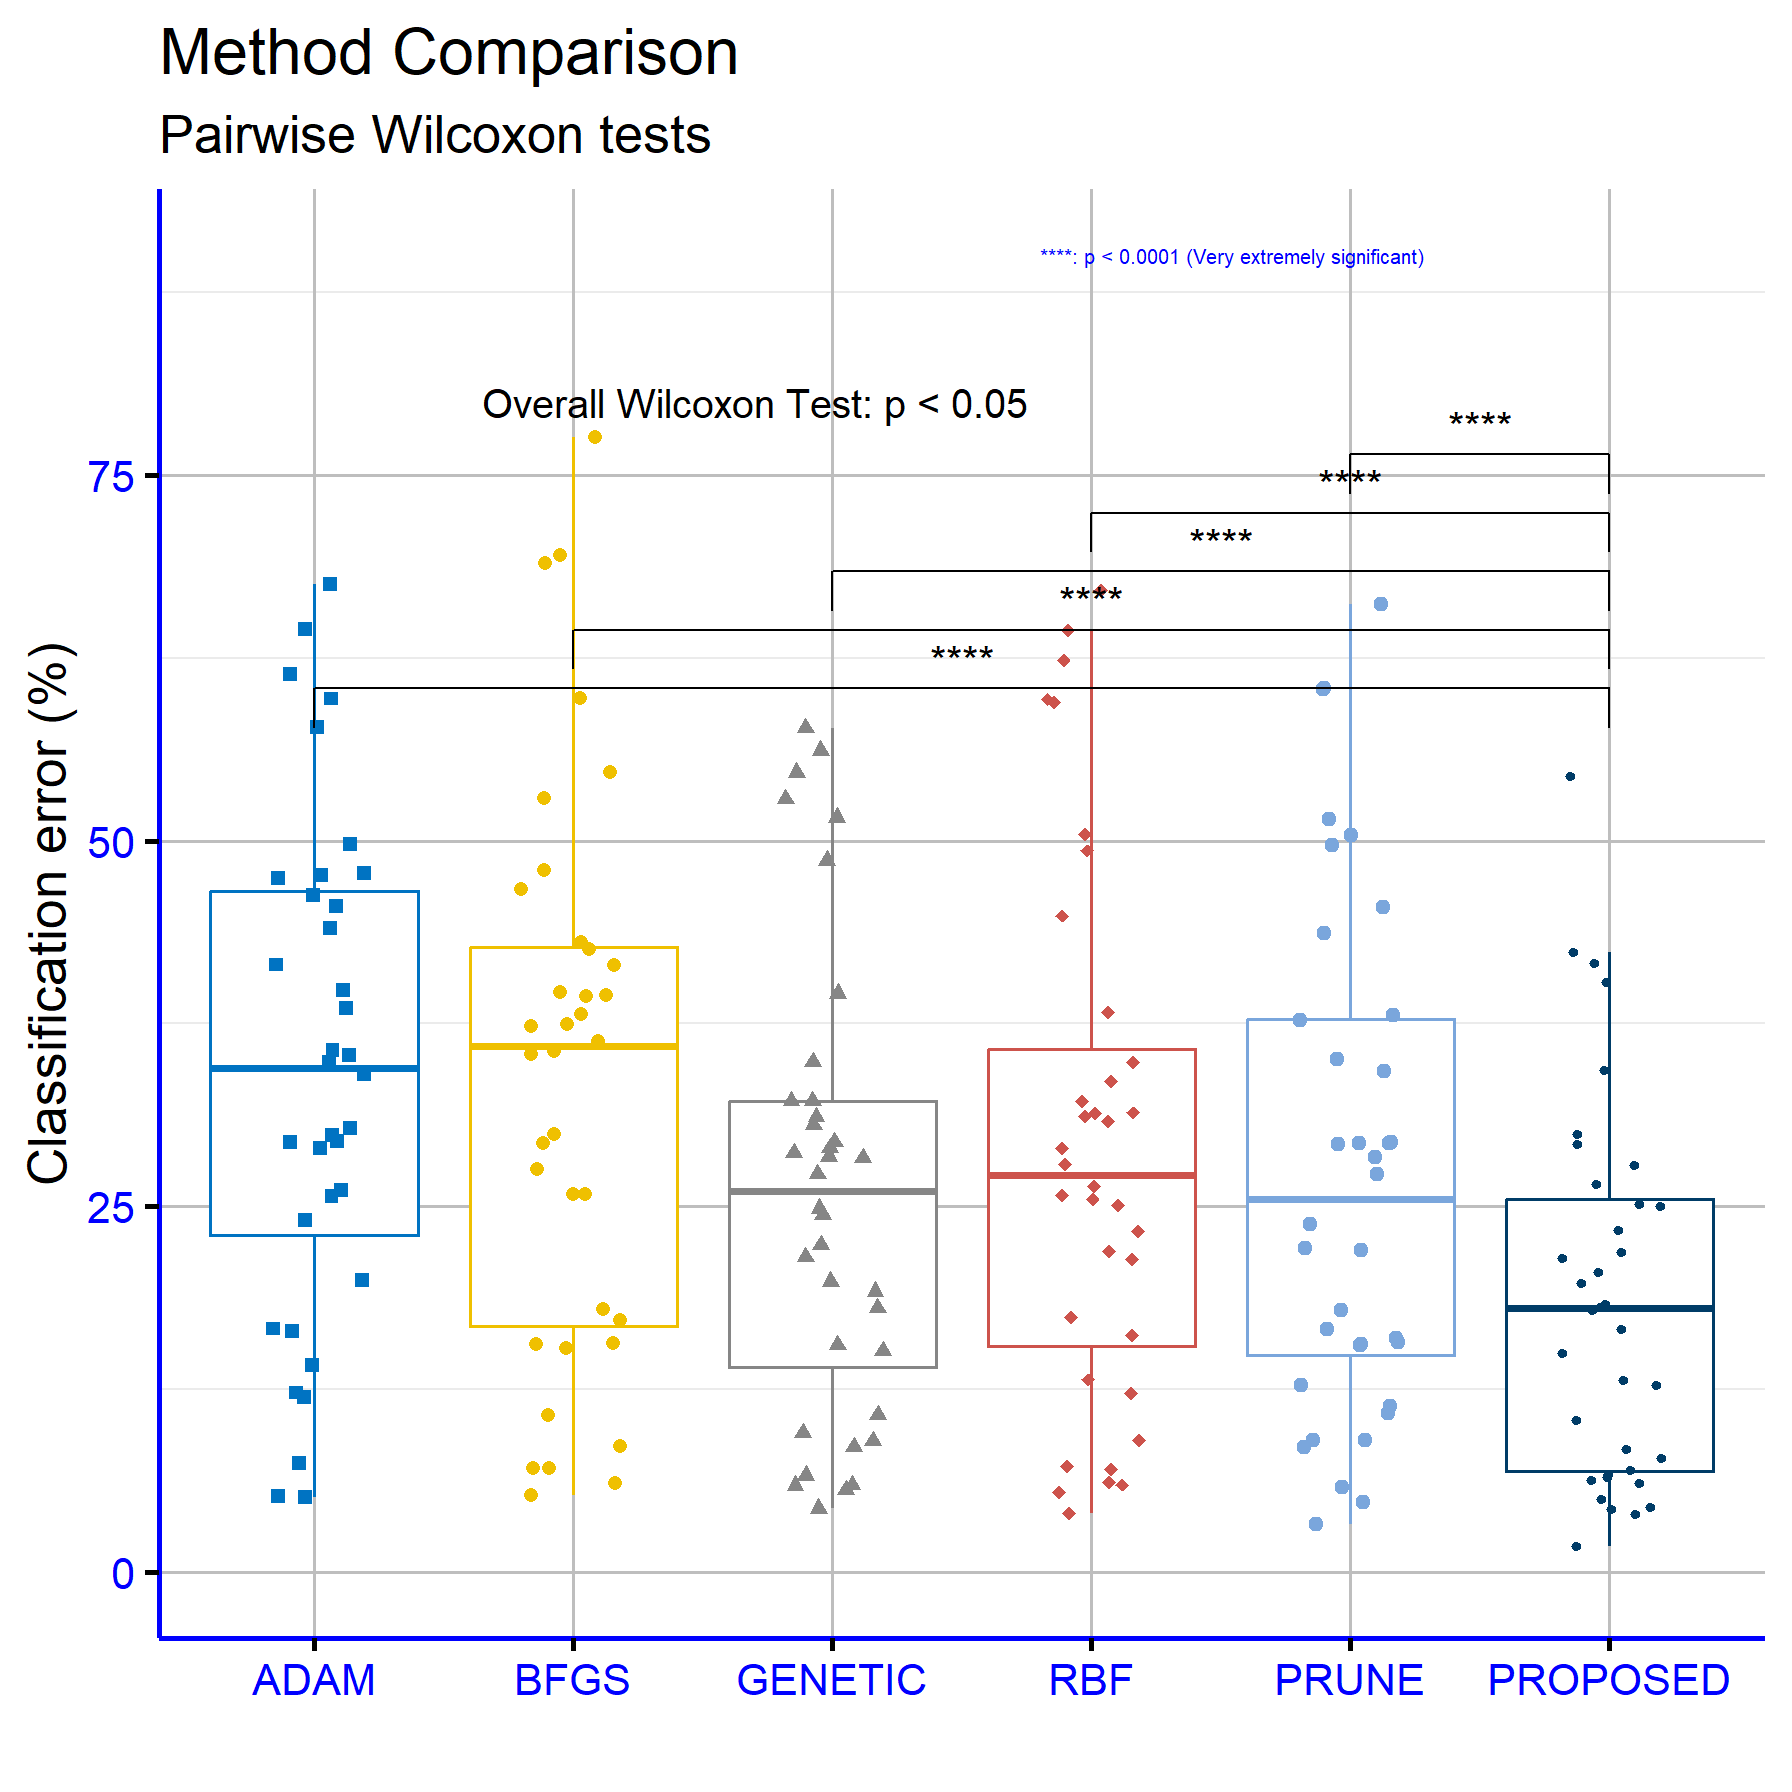
\includegraphics[scale=0.5]{img1}
\par\end{centering}
\caption{Statistical comparison of the used methods for the classification
datasets.\protect\label{fig:statClass}}
\end{figure}

Consequently, the results from Figure \ref{fig:statRegression} further
strengthen the position of the PROPOSED model as the most effective
solution for regression problems, providing reliable and statistically
significant performance.

\begin{figure}[H]
\begin{centering}
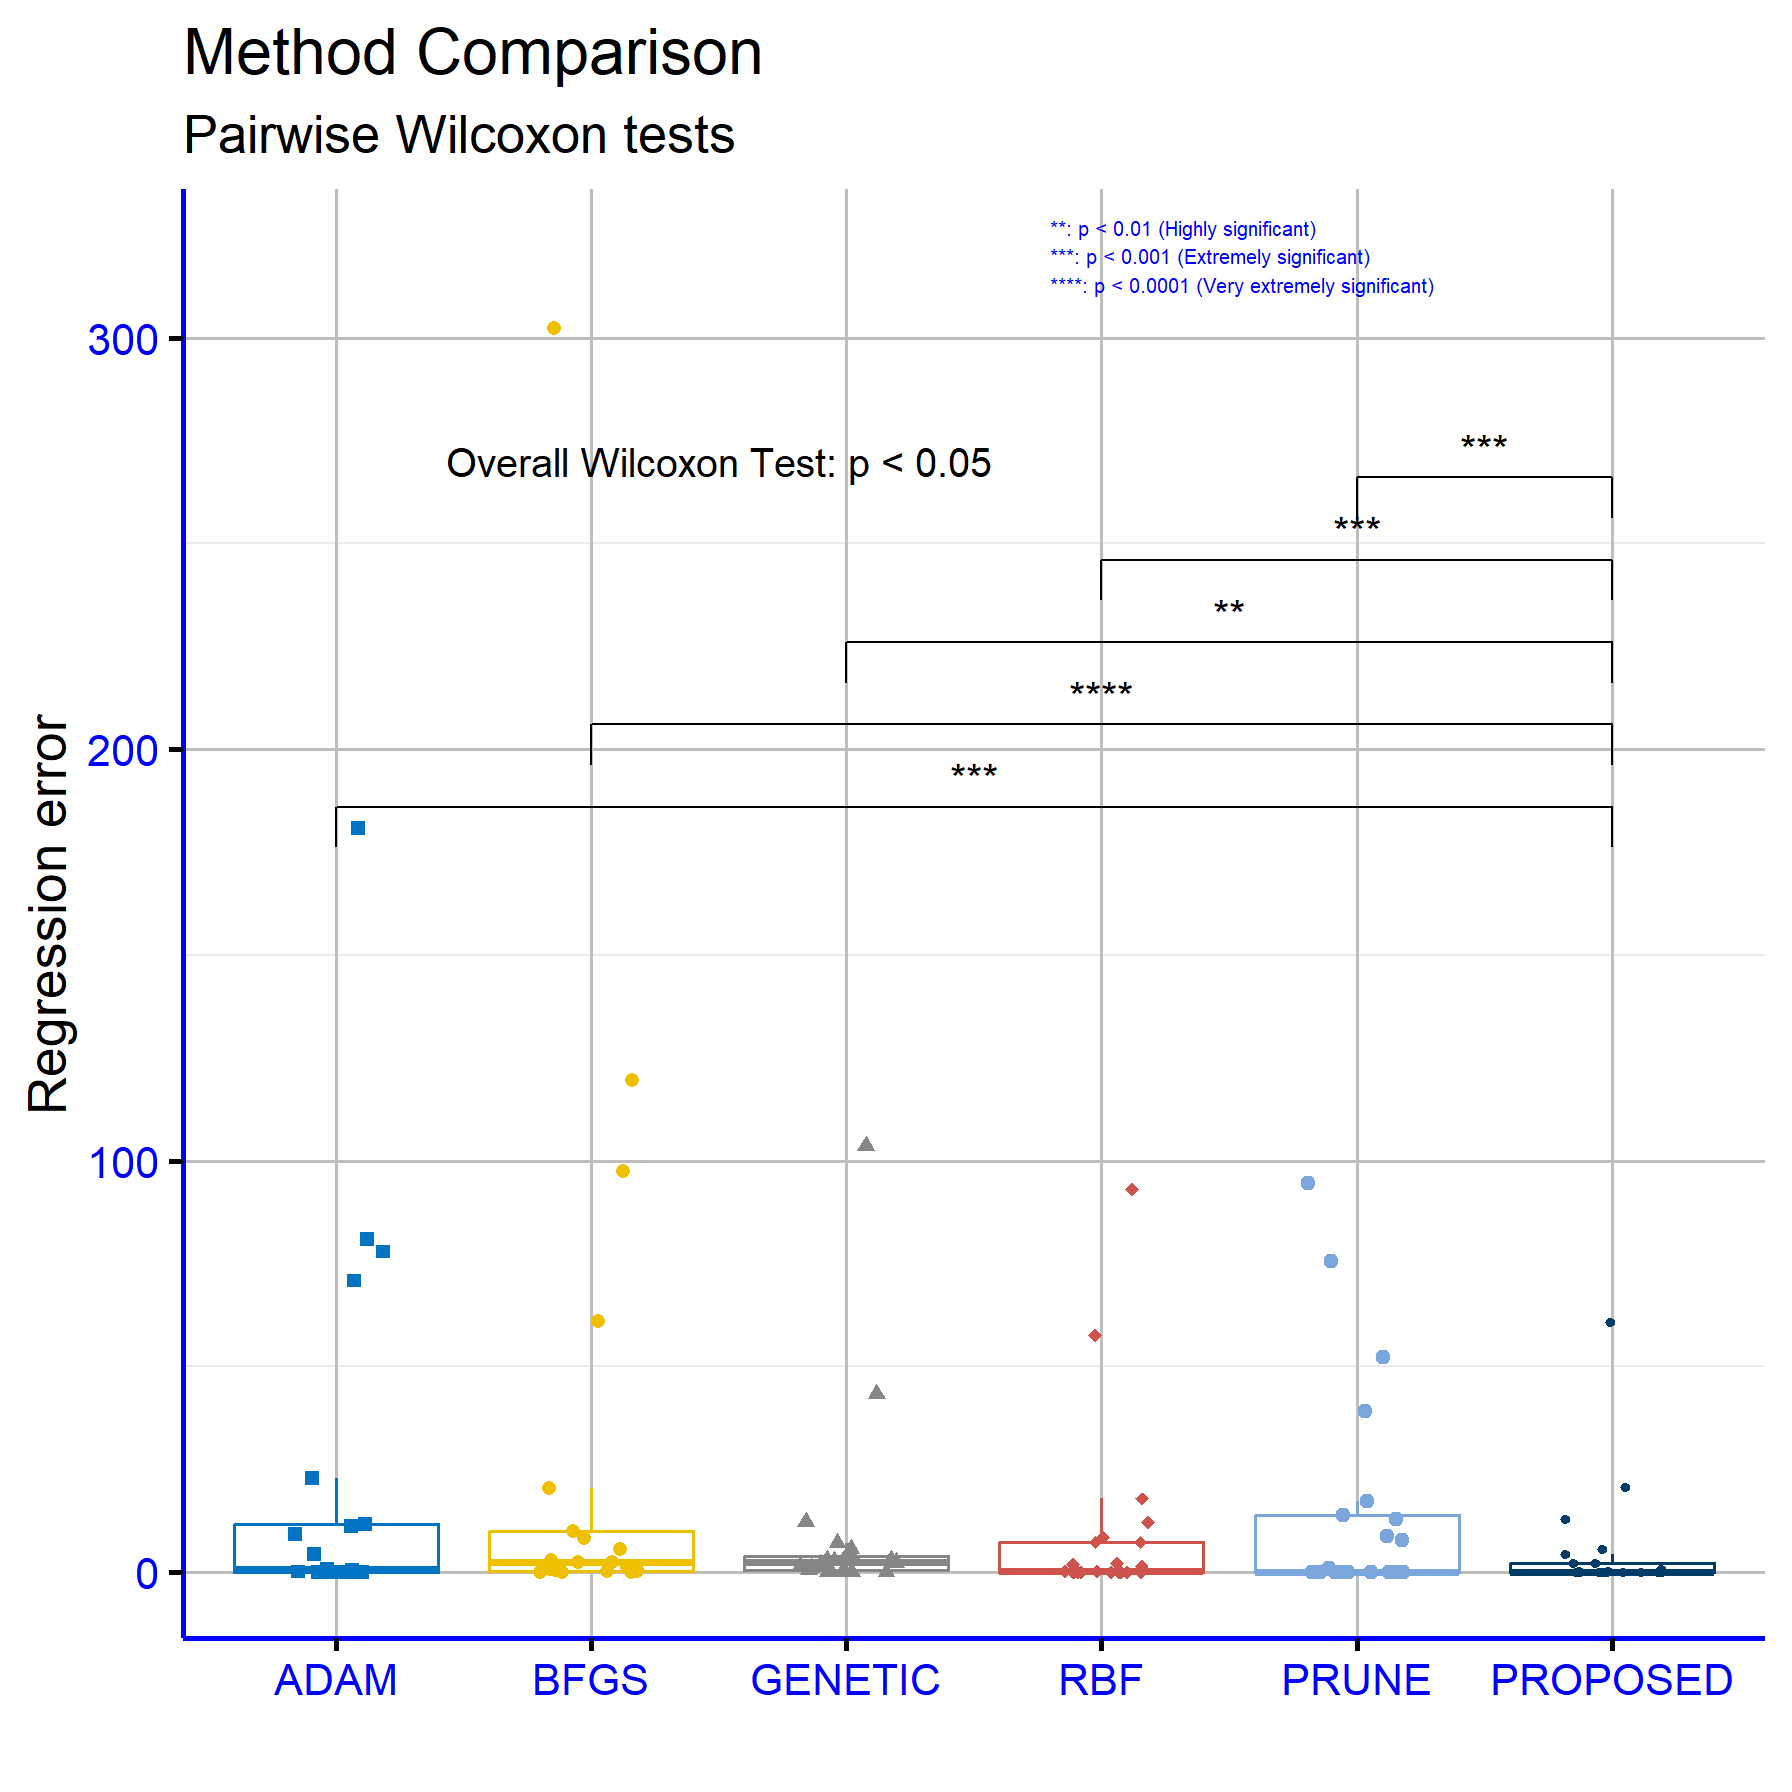
\includegraphics[scale=0.5]{img2}
\par\end{centering}
\caption{Statistical comparison between the used methods for the regression
datasets.\protect\label{fig:statRegression}}

\end{figure}
 Also, in the plot of Figure \ref{fig:comparisonDermatology}a comparison
in terms of classification error is made between the simple genetic
algorithm and the proposed one for the Dermatology dataset. Likewise,
in Figure \ref{fig:comparisonHousing} a plot of the regression error
is outlined for the genetic algorithm and the proposed method. For
both cases, there is a significant improvement in terms of error values.

\begin{figure}[H]
\begin{centering}
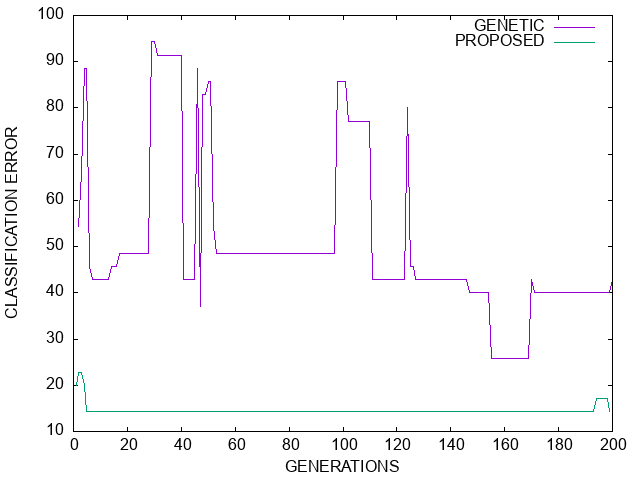
\includegraphics[scale=0.5]{dermatology_plot}
\par\end{centering}
\caption{A graphical comparison of the genetic algorithm and the proposed method
for the Dermatology dataset. The horizontal axis denotes number of
generations and the vertical classification error as measured on the
test set.\protect\label{fig:comparisonDermatology}}

\end{figure}
\begin{figure}[H]
\begin{centering}
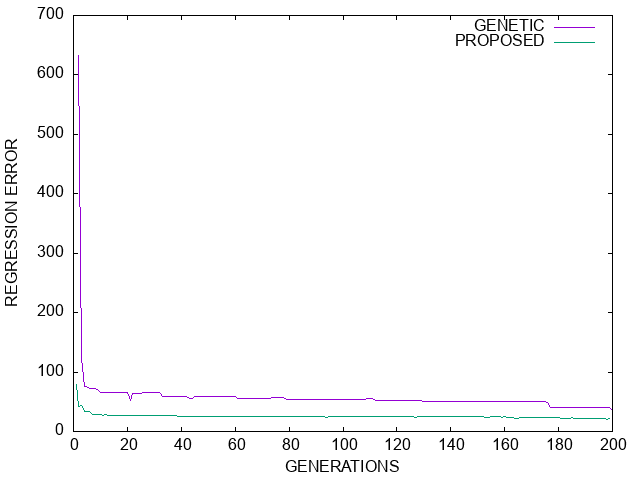
\includegraphics[scale=0.5]{housing_plot}
\par\end{centering}
\caption{Comparison between the genetic algorithm and the proposed method for
the Housing regression dataset.The horizontal axis denotes number
of generations and the vertical regression error as measured on the
test set.\protect\label{fig:comparisonHousing}}
\end{figure}


\subsection{Using different weight methods}

An additional experiment was executed where the parameter $F$ of
the differential evolution was altered using some well - known approaches
from the relevant literature. In the following tables the following
methods, as denoted in the experimental tables, were obtained for
the calculation of the parameter $F$:
\begin{enumerate}
\item RANDOM. This method is used for the current approach, where the differential
weight is a random number in $[0,1]$.
\item FIXED. This method is used when the value for $F$ is used, as denoted
in Table \ref{tab:settings}.
\item ADAPT. This method is used for the adaptive calculation of parameter
$F$ as proposed in \citep{de_adaptive}.
\item MIGRANT. For this case the calculation for parameter $F$ as proposed
in \citep{de_migrant} is adopted.
\end{enumerate}
The experimental results using the current method and the previously
mentioned method for differential weight are listed in Tables \ref{tab:experFClass}
and \ref{tab:experFRegression} for the classification datasets and
the regression datasets respectively.

\begin{table}[H]
\caption{Experimental results for the classification datasets and the proposed
method using a series of differential weight mechanisms.\protect\label{tab:experFClass}}

\centering{}%
\begin{tabular}{|c|c|c|c|c|}
\hline 
DATASET & RANDOM & FIXED & ADAPT & MIGRANT\tabularnewline
\hline 
\hline 
APPENDICITIS & 15.00\% & 14.90\% & 15.30\% & 15.80\%\tabularnewline
\hline 
ALCOHOL & 18.33\% & 20.81\% & 22.08\% & 17.26\%\tabularnewline
\hline 
AUSTRALIAN & 21.49\% & 19.62\% & 23.91\% & 29.49\%\tabularnewline
\hline 
BALANCE & 7.79\% & 7.56\% & 8.39\% & 8.39\%\tabularnewline
\hline 
CLEVELAND & 42.38\% & 42.31\% & 41.79\% & 44.79\%\tabularnewline
\hline 
CIRCULAR & 6.50\% & 7.24\% & 7.40\% & 4.74\%\tabularnewline
\hline 
DERMATOLOGY & 4.97\% & 5.72\% & 5.71\% & 11.40\%\tabularnewline
\hline 
ECOLI & 40.30\% & 42.18\% & 45.51\% & 47.61\%\tabularnewline
\hline 
GLASS & 54.38\% & 54.33\% & 56.29\% & 49.00\%\tabularnewline
\hline 
HABERMAN & 26.53\% & 27.93\% & 30.00\% & 26.60\%\tabularnewline
\hline 
HAYES-ROTH & 34.31\% & 34.00\% & 28.62\% & 35.00\%\tabularnewline
\hline 
HEART & 13.11\% & 15.30\% & 14.56\% & 19.04\%\tabularnewline
\hline 
HEARTATTACK & 21.90\% & 19.57\% & 20.00\% & 20.70\%\tabularnewline
\hline 
HOUSEVOTES & 6.09\% & 6.00\% & 5.22\% & 5.48\%\tabularnewline
\hline 
IONOSPHERE & 10.37\% & 9.71\% & 8.86\% & 11.80\%\tabularnewline
\hline 
LIVERDISORDER & 29.94\% & 30.97\% & 29.56\% & 31.12\%\tabularnewline
\hline 
LYMOGRAPHY & 17.93\% & 18.93\% & 20.72\% & 20.93\%\tabularnewline
\hline 
MAMMOGRAPHIC & 16.63\% & 15.74\% & 16.12\% & 17.50\%\tabularnewline
\hline 
PARKINSONS & 12.79\% & 9.69\% & 11.58\% & 14.42\%\tabularnewline
\hline 
PHONEME & 18.10\% & 17.23\% & 18.15\% & 18.40\%\tabularnewline
\hline 
PIMA & 25.03\% & 27.66\% & 27.89\% & 27.70\%\tabularnewline
\hline 
POPFAILURES & 4.45\% & 5.19\% & 4.82\% & 4.39\%\tabularnewline
\hline 
REGIONS2 & 25.19\% & 25.03\% & 23.24\% & 30.92\%\tabularnewline
\hline 
SAHEART & 29.26\% & 32.26\% & 30.76\% & 32.28\%\tabularnewline
\hline 
SEGMENT & 27.80\% & 36.29\% & 33.83\% & 42.80\%\tabularnewline
\hline 
SONAR & 20.50\% & 20.85\% & 21.00\% & 22.10\%\tabularnewline
\hline 
SPIRAL & 41.60\% & 43.93\% & 45.67\% & 44.04\%\tabularnewline
\hline 
STATHEART & 19.74\% & 18.52\% & 16.67\% & 17.41\%\tabularnewline
\hline 
STUDENT & 4.00\% & 4.38\% & 4.25\% & 4.63\%\tabularnewline
\hline 
TRANSFUSION & 23.35\% & 22.95\% & 24.58\% & 23.50\%\tabularnewline
\hline 
WDBC & 6.73\% & 6.48\% & 7.50\% & 4.18\%\tabularnewline
\hline 
WINE & 6.29\% & 5.82\% & 6.35\% & 11.59\%\tabularnewline
\hline 
Z\_F\_S & 8.38\% & 7.00\% & 9.27\% & 10.43\%\tabularnewline
\hline 
ZO\_NF\_S & 4.32\% & 5.52\% & 6.00\% & 8.36\%\tabularnewline
\hline 
ZONF\_S & 1.76\% & 1.92\% & 2.20\% & 2.32\%\tabularnewline
\hline 
ZOO & 7.00\% & 4.90\% & 9.00\% & 6.10\%\tabularnewline
\hline 
\textbf{AVERAGE} & \textbf{18.73\%} & \textbf{19.12\%} & \textbf{19.52\%} & \textbf{20.62\%}\tabularnewline
\hline 
\end{tabular}
\end{table}
\begin{table}[H]
\caption{Experimental results for the regression datasets and the proposed
method using a variety of techniques for the calculation of differential
weight.\protect\label{tab:experFRegression}}

\centering{}%
\begin{tabular}{|c|c|c|c|c|}
\hline 
DATASET & RANDOM & FIXED & ADAPT & MIGRANT\tabularnewline
\hline 
\hline 
ABALONE & 4.32 & 4.47 & 4.35 & 4.41\tabularnewline
\hline 
AIRFOIL & 0.002 & 0.003 & 0.003 & 0.003\tabularnewline
\hline 
AUTO & 12.78 & 13.58 & 13.98 & 11.46\tabularnewline
\hline 
BK & 0.02 & 0.057 & 0.021 & 0.021\tabularnewline
\hline 
BL & 0.006 & 0.008 & 0.006 & 0.008\tabularnewline
\hline 
BASEBALL & 60.74 & 65.12 & 67.71 & 60.10\tabularnewline
\hline 
CONCRETE & 0.006 & 0.026 & 0.007 & 0.004\tabularnewline
\hline 
DEE & 0.19 & 0.21 & 0.20 & 0.24\tabularnewline
\hline 
FRIEDMAN & 2.21 & 2.79 & 3.18 & 1.88\tabularnewline
\hline 
FY & 0.067 & 0.046 & 0.042 & 0.052\tabularnewline
\hline 
HO & 0.015 & 0.017 & 0.052 & 0.013\tabularnewline
\hline 
HOUSING & 20.74 & 24.63 & 24.83 & 24.71\tabularnewline
\hline 
LASER & 0.004 & 0.004 & 0.004 & 0.003\tabularnewline
\hline 
LW & 0.011 & 0.014 & 0.011 & 0.013\tabularnewline
\hline 
MORTGAGE & 0.32 & 0.71 & 0.32 & 0.22\tabularnewline
\hline 
PL & 0.022 & 0.022 & 0.022 & 0.023\tabularnewline
\hline 
PLASTIC & 2.16 & 2.15 & 2.15 & 2.36\tabularnewline
\hline 
QUAKE & 0.036 & 0.052 & 0.036 & 0.044\tabularnewline
\hline 
SN & 0.023 & 0.036 & 0.025 & 0.024\tabularnewline
\hline 
STOCK & 5.57 & 5.89 & 4.72 & 4.41\tabularnewline
\hline 
TREASURY & 0.68 & 0.64 & 0.51 & 0.65\tabularnewline
\hline 
\textbf{AVERAGE} & \textbf{5.23} & \textbf{5.74} & \textbf{5.82} & \textbf{5.27}\tabularnewline
\hline 
\end{tabular}
\end{table}

The statistical analysis of Table \ref{tab:experFClass} examines
the percentage error rates across various classification datasets
using four different computations of the critical weight differential
parameter for the proposed machine learning model: RANDOM, FIXED,
ADAPT, and MIGRANT. The RANDOM computation exhibits the lowest overall
average error rate (18.73\%), indicating superior performance compared
to the other computations: FIXED (19.12\%), ADAPT (19.52\%), and MIGRANT
(20.62\%). This suggests that the RANDOM computation is the most reliable
overall. Analyzing individual datasets, the RANDOM computation achieves
the best error rates in several cases. For instance, it records the
lowest error rates for datasets such as \textquotedbl ALCOHOL\textquotedbl{}
(18.33\%), \textquotedbl BALANCE\textquotedbl{} (7.79\%), \textquotedbl CIRCULAR\textquotedbl{}
(6.50\%), \textquotedbl HOUSEVOTES\textquotedbl{} (6.09\%), \textquotedbl PARKINSONS\textquotedbl{}
(12.79\%), \textquotedbl POPFAILURES\textquotedbl{} (4.45\%), and
\textquotedbl WDBC\textquotedbl{} (6.73\%). These results highlight
its effectiveness across a wide range of datasets. Specifically, the
4.45\% error rate for \textquotedbl POPFAILURES\textquotedbl{} stands
out as one of the lowest overall. In certain datasets, the FIXED computation
outperforms others, such as in \textquotedbl Z\_F\_S\textquotedbl{}
(7.00\%) and \textquotedbl ZOO\textquotedbl{} (4.90\%). However,
the difference from RANDOM is minimal. The MIGRANT computation demonstrates
the lowest error rates in only a few cases, such as \textquotedbl CIRCULAR\textquotedbl{}
(4.74\%) and \textquotedbl WDBC\textquotedbl{} (4.18\%), suggesting
it may be particularly effective for specific datasets. Meanwhile,
the ADAPT computation achieves lower error rates in a few scenarios
but generally remains less competitive. In other datasets, such as
\textquotedbl GLASS,\textquotedbl{} \textquotedbl SPIRAL,\textquotedbl{}
and \textquotedbl SEGMENT,\textquotedbl{} all computations show high
error rates, indicating these datasets are challenging to classify
regardless of the computation. Nevertheless, the RANDOM computation
remains consistently competitive even with these difficult datasets,
as observed in \textquotedbl STATHEART\textquotedbl{} and \textquotedbl ZONF\_S.\textquotedbl{}
In conclusion, the analysis reveals that the RANDOM computation is
the most effective overall, achieving the lowest average error rate
and demonstrating superior performance across a broad range of datasets.
However, there are instances where other computations, such as FIXED
and MIGRANT, show specialized advantages.

The statistical analysis of Table \ref{tab:experFRegression} pertains
to regression datasets, using four different calculations of the critical
parameter of differential weighting for the proposed machine learning
model: RANDOM, FIXED, ADAPT, and MIGRANT. The RANDOM calculation exhibits
the lowest average error (5.23), making it the most efficient overall
compared to FIXED (5.74), ADAPT (5.82), and MIGRANT (5.27). The small
difference between RANDOM and MIGRANT suggests comparable performance
between these two approaches, with RANDOM maintaining a slight edge.
For individual datasets, the RANDOM calculation achieves the lowest
error values in several cases, such as the \textquotedbl AUTO\textquotedbl{}
(12.78), \textquotedbl FRIEDMAN\textquotedbl{} (2.21), \textquotedbl HO\textquotedbl{}
(0.015), \textquotedbl MORTGAGE\textquotedbl{} (0.32), and \textquotedbl SN\textquotedbl{}
(0.023) datasets. These results demonstrate the effectiveness of the
RANDOM calculation across a wide range of datasets. In the \textquotedbl FRIEDMAN\textquotedbl{}
dataset, the error value of 2.21 is significantly lower than the corresponding
values of FIXED (2.79) and ADAPT (3.18), underscoring its performance
in this specific dataset. The MIGRANT calculation demonstrates the
best performance in certain datasets, such as \textquotedbl AUTO\textquotedbl{}
(11.46) and \textquotedbl STOCK\textquotedbl{} (4.41), where it outperforms
RANDOM. However, in other datasets, such as \textquotedbl PLASTIC\textquotedbl{}
and \textquotedbl SN,\textquotedbl{} it shows slightly higher error
rates, indicating limitations with specific data. The FIXED calculation
tends to have consistent but not top-performing results, while ADAPT
generally shows higher error values, making it less effective overall.
In summary, the analysis highlights that the RANDOM calculation is
the most reliable and efficient, with the lowest average error and
strong performance across various datasets. However, the MIGRANT calculation
exhibits competitive performance in specific cases, while FIXED and
ADAPT appear to require improvements to rival the other calculations.

Figure \ref{fig:statFClass} evaluates classification datasets for
different differential weight computations within the proposed machine
learning model. The p-values are as follows: RANDOM vs FIXED: p=0.43,
RANDOM vs ADAPT: p=0.024, RANDOM vs MIGRANT: p=0.0021, FIXED vs ADAPT
p=0.12, FIXED vs MIGRANT: p=0.0033 and ADAPT vs MIGRANT: p=0.043.
These results suggest that some comparisons, such as RANDOM vs MIGRANT
and FIXED vs MIGRANT, show strong statistical significance, while
others, such as RANDOM vs FIXED, do not demonstrate significant differences. 

\begin{figure}[H]
\begin{centering}
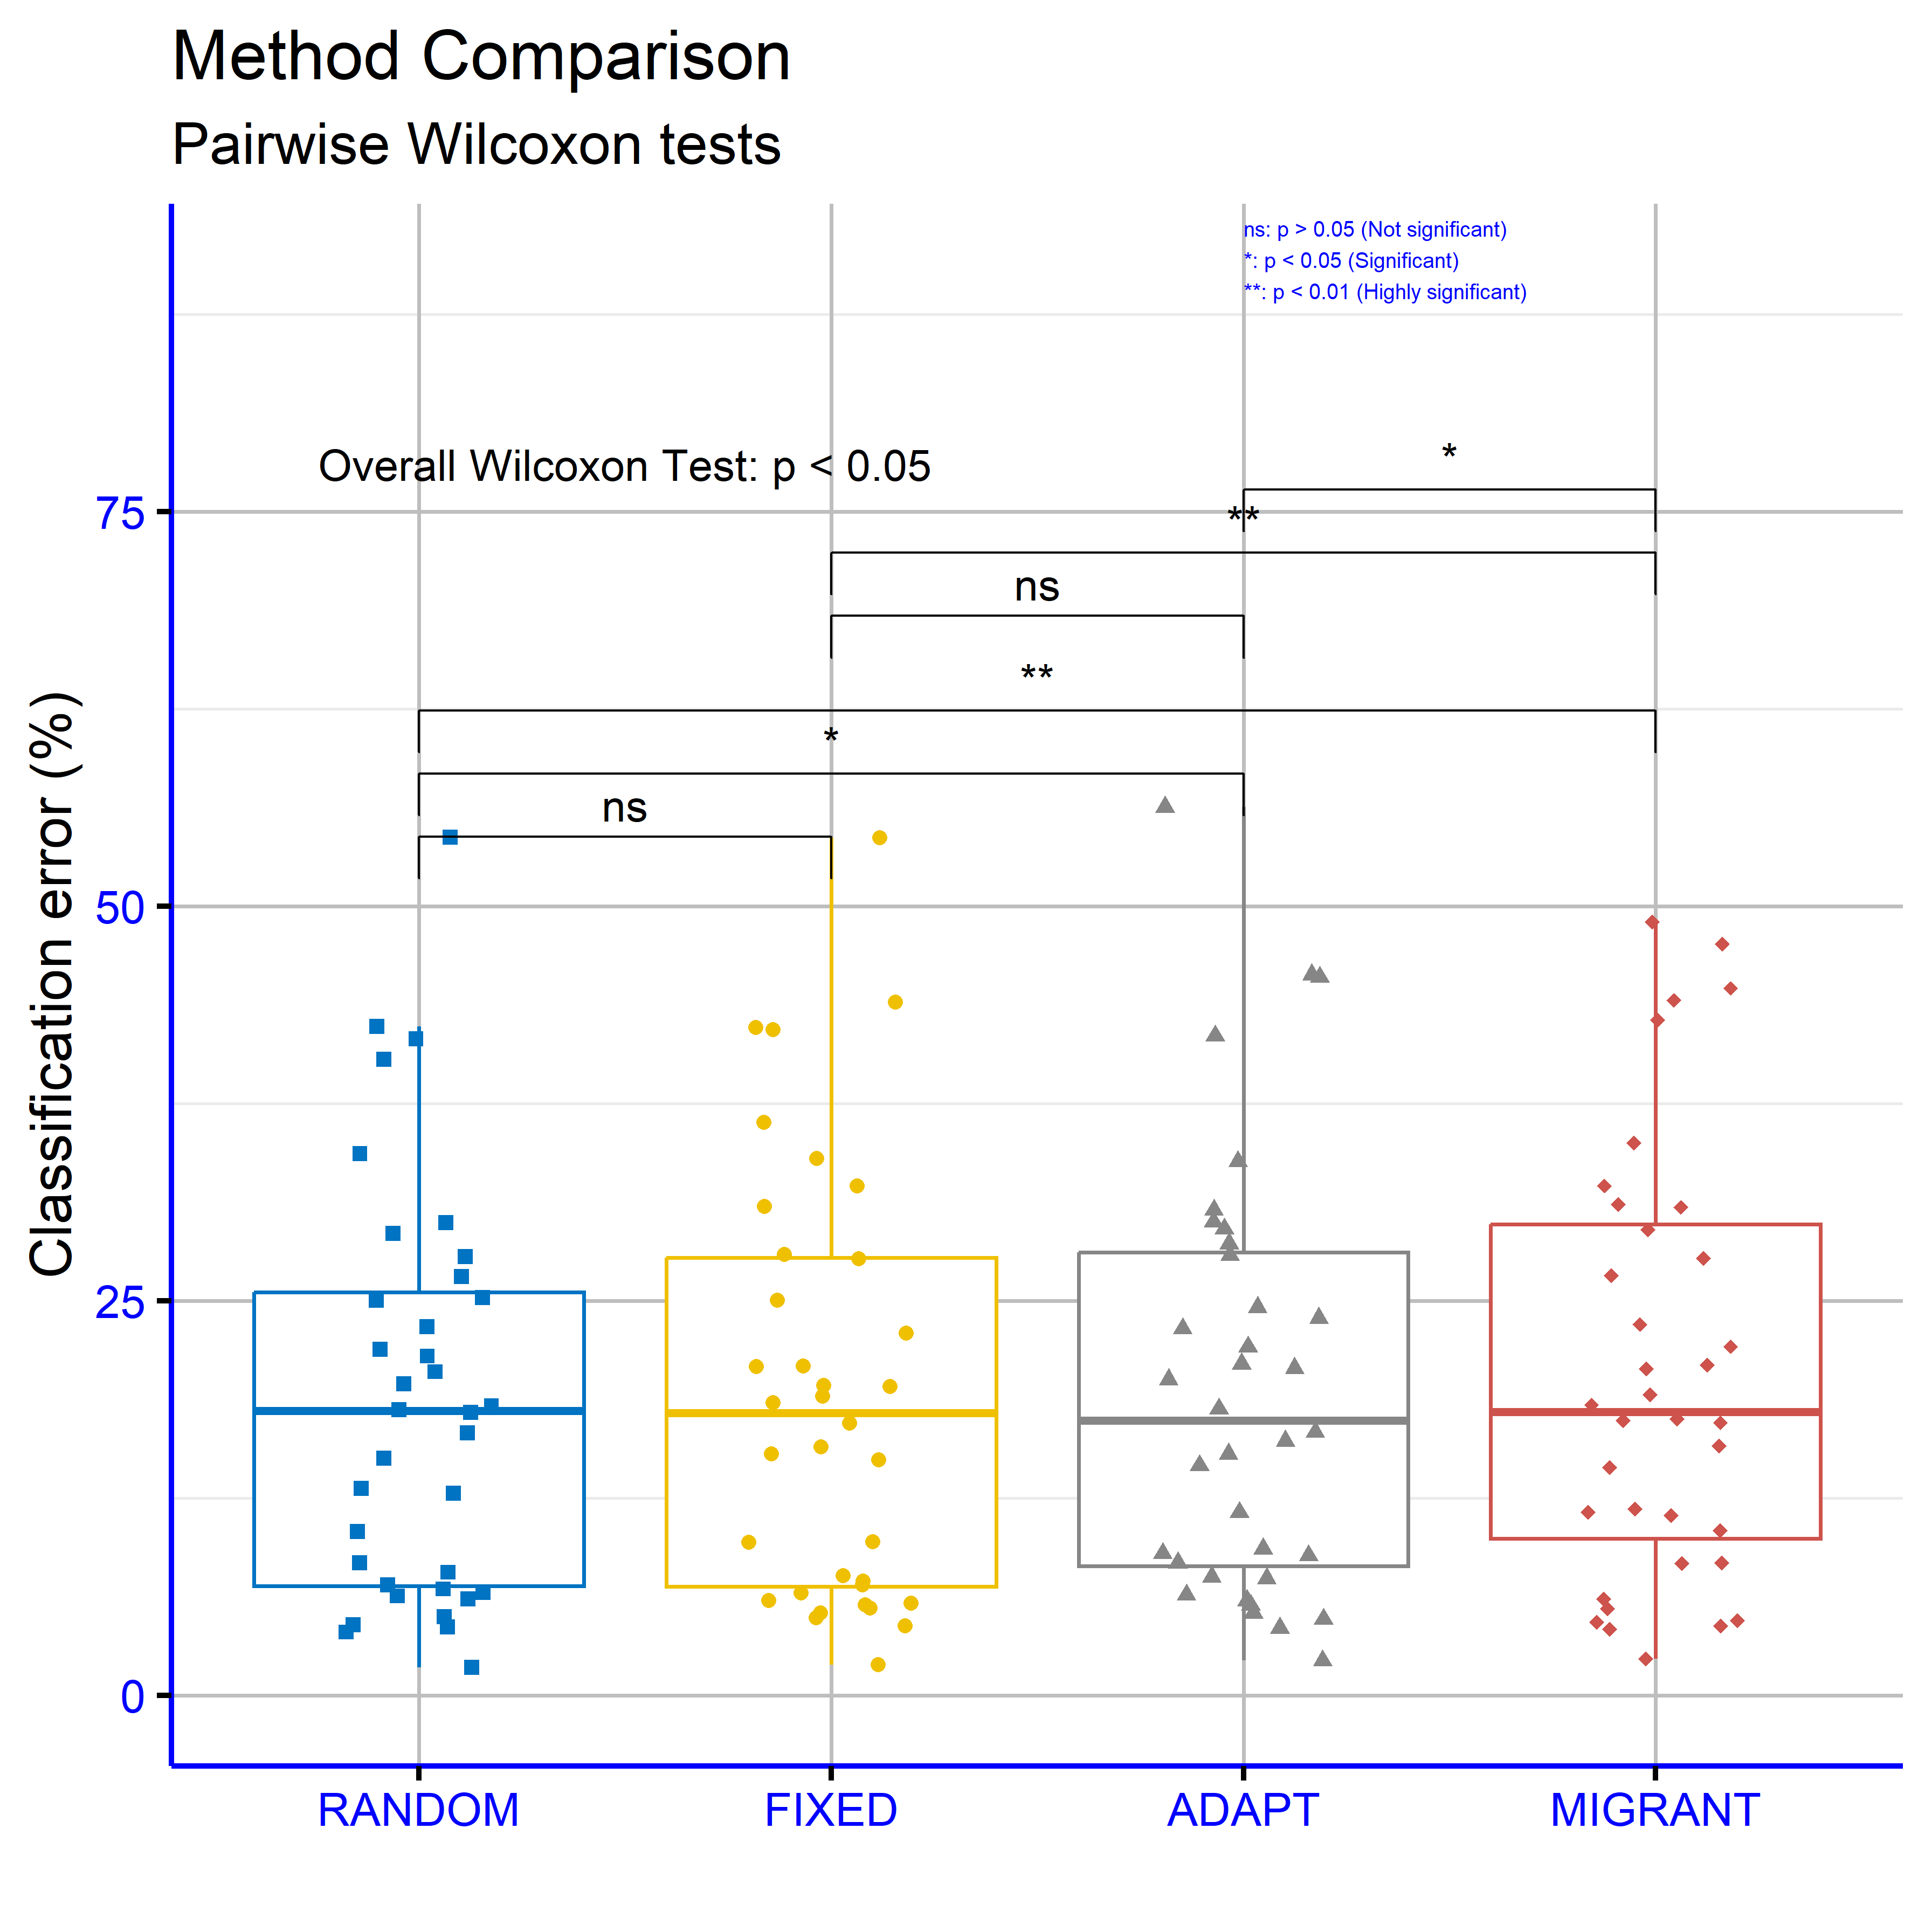
\includegraphics[scale=0.5]{img3}
\par\end{centering}
\caption{Statistical comparison between the proposed variations of the differential
weight mechanisms. The experiments were conducted on the classification
datasets.\protect\label{fig:statFClass}}

\end{figure}

Figure \ref{fig:statFRegression} presents results for regression
datasets using different differential weight computations within the
proposed model. The observed p-values are: RANDOM vs FIXED: p=0.0066,
RANDOM vs ADAPT: p=0.15, RANDOM vs MIGRANT: p=0.66, FIXED vs ADAPT:
p=0.64, FIXED vs MIGRANT: p=0.84 and ADAPT vs MIGRANT: p=0.47. These
findings indicate that most comparisons do not show significant differences,
except for RANDOM vs FIXED, which demonstrates a notable level of
significance. 

\begin{figure}[H]
\begin{centering}
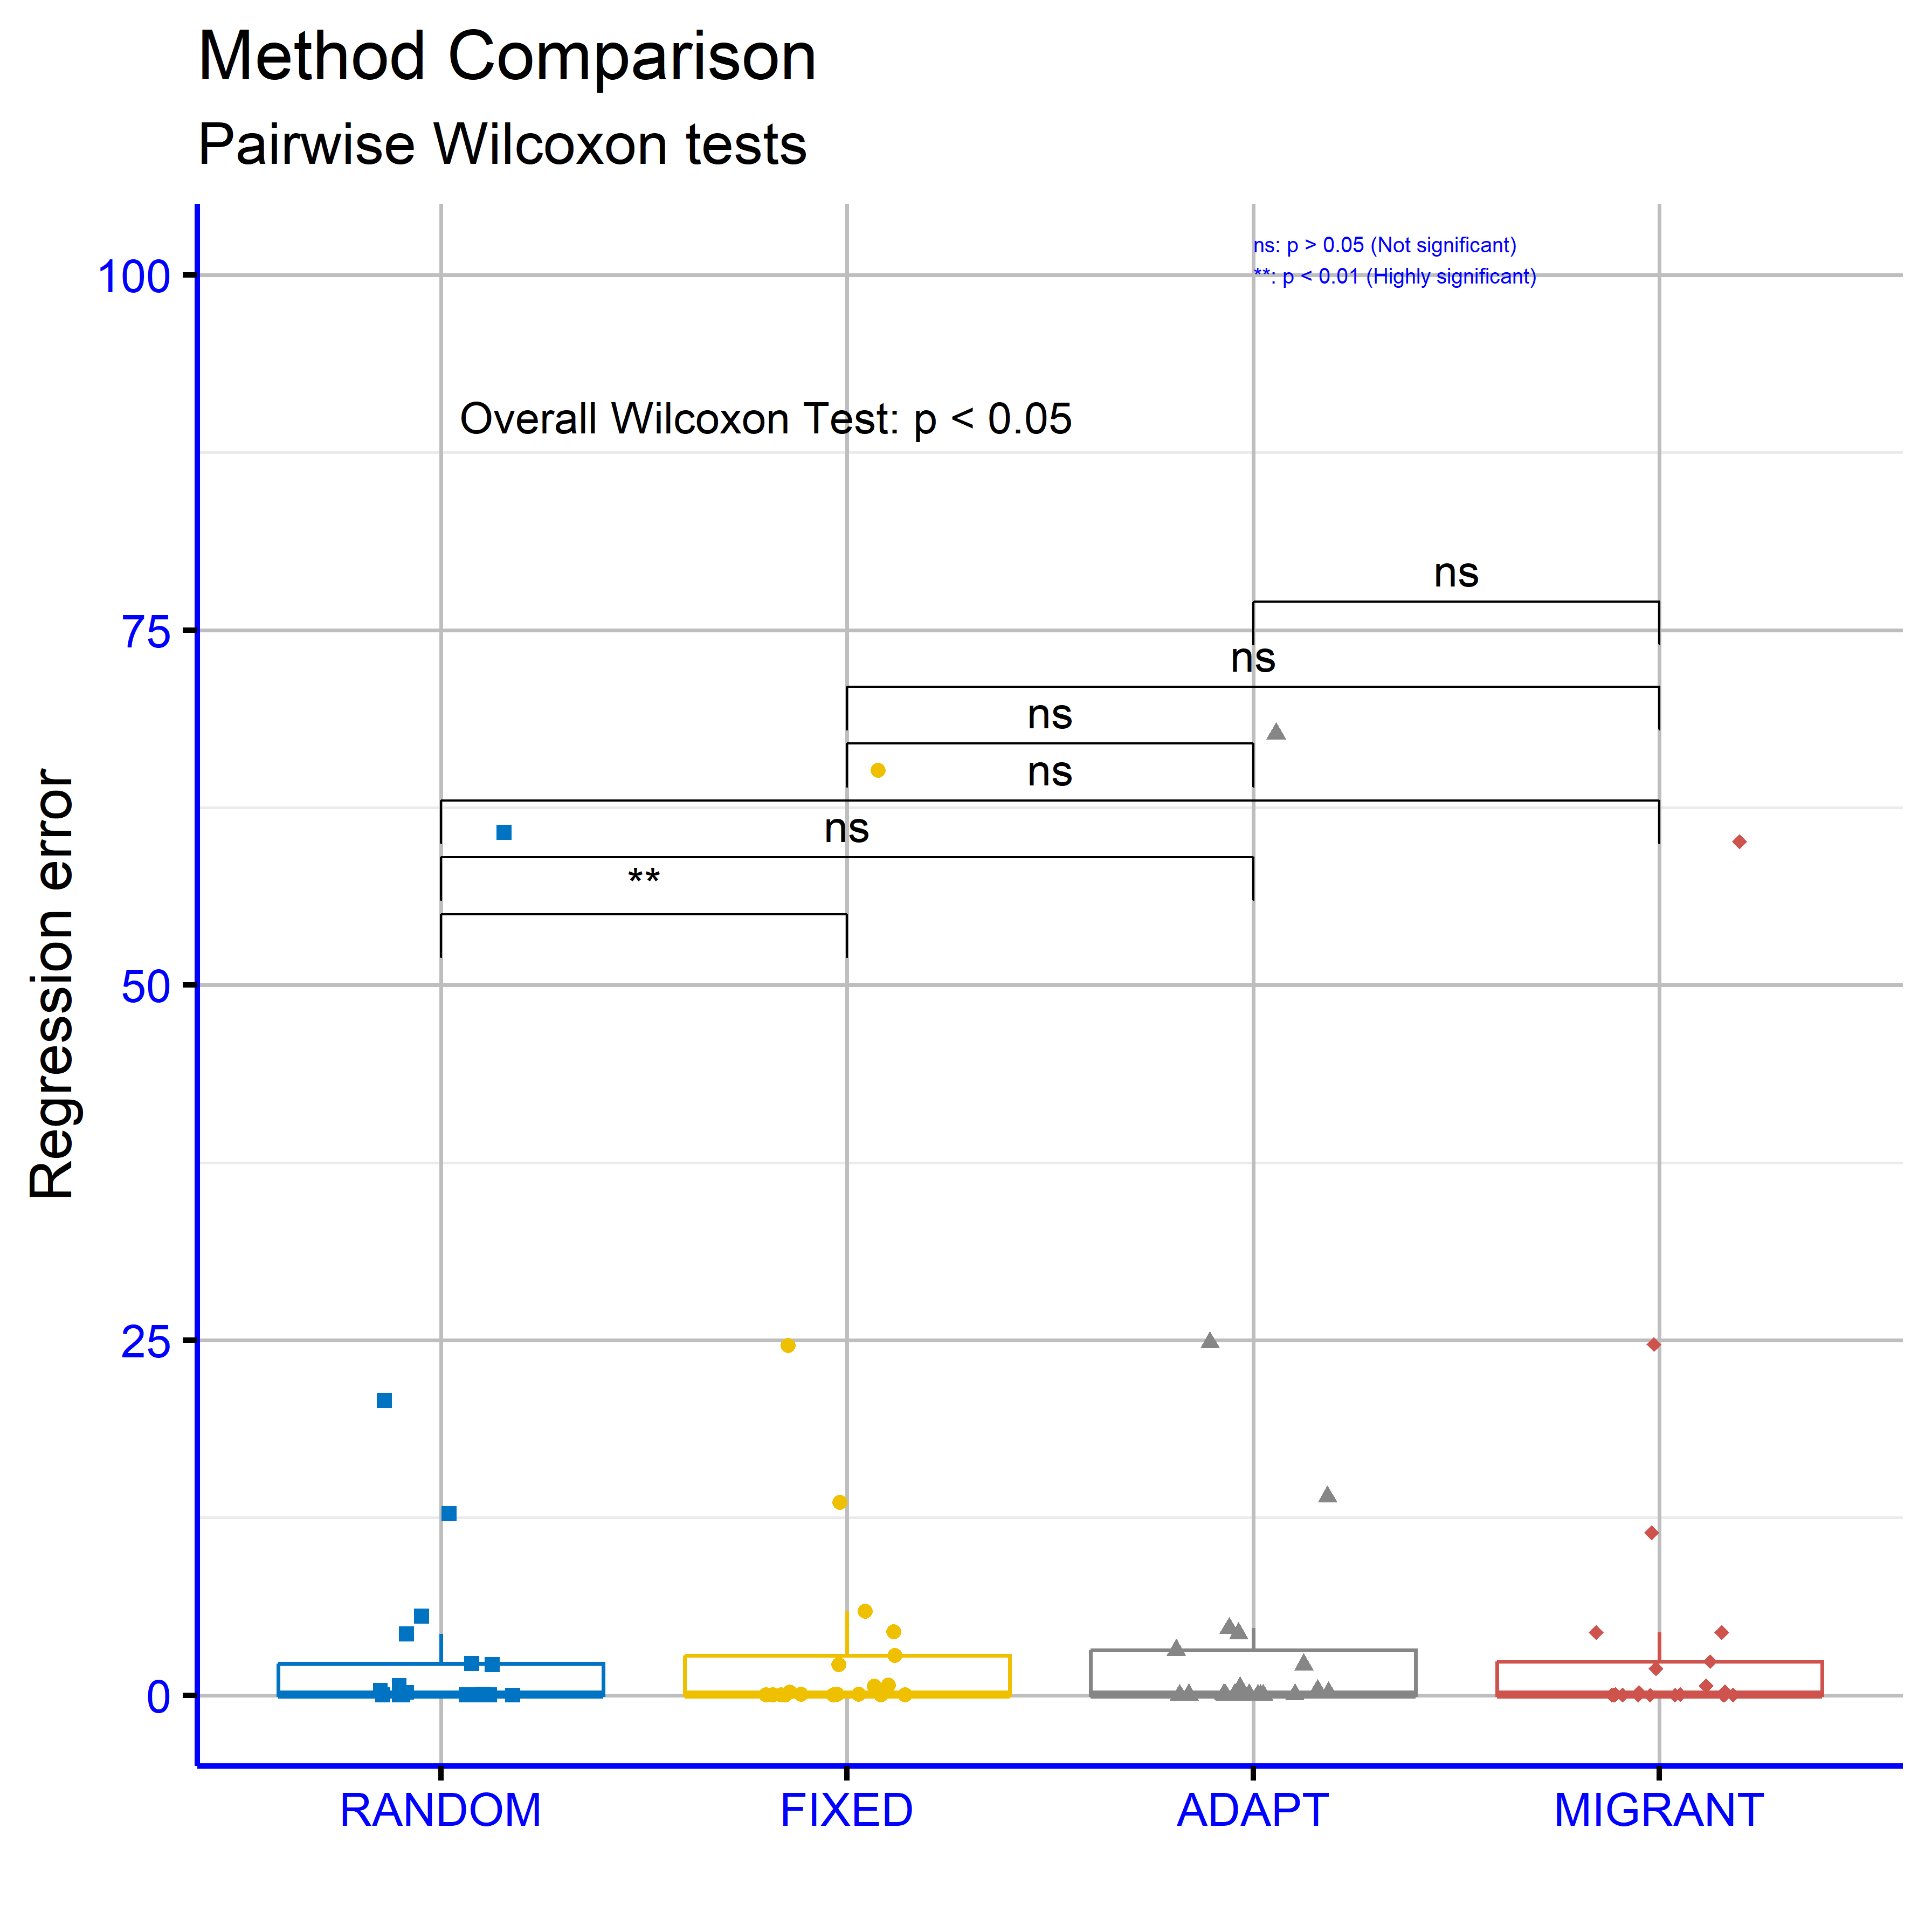
\includegraphics[scale=0.5]{img4}
\par\end{centering}
\caption{Statistical comparison for the different variations of the weight
calculation mechanism. The experiments were conducted using the proposed
method on the regression datasets.\protect\label{fig:statFRegression}}

\end{figure}


\subsection{Experiment with the number of agents}

An additional experiment was conducted using different values for
the parameter NP, which represents the number of agents. In this experiment
the parameter NP took the values 50, 100 and 200. The experimental
results for the classification datasets are shown in Table \ref{tab:experNPClass}
and for the regression datasets in Table \ref{tab:experNPRegression}.

\begin{table}[H]

\caption{Experimental results for the classification datasets and the proposed
method using a variety of values for the parameter NP.\protect\label{tab:experNPClass}}

\centering{}%
\begin{tabular}{|c|c|c|c|}
\hline 
DATASET & NP=50 & NP=100 & NP=200\tabularnewline
\hline 
\hline 
APPENDICITIS & 14.00\% & 14.00\% & 15.00\%\tabularnewline
\hline 
ALCOHOL & 26.90\% & 25.36\% & 18.33\%\tabularnewline
\hline 
AUSTRALIAN & 30.67\% & 25.83\% & 21.49\%\tabularnewline
\hline 
BALANCE & 7.42\% & 8.13\% & 7.79\%\tabularnewline
\hline 
CLEVELAND & 39.55\% & 42.10\% & 42.38\%\tabularnewline
\hline 
CIRCULAR & 8.50\% & 6.79\% & 6.50\%\tabularnewline
\hline 
DERMATOLOGY & 9.89\% & 11.34\% & 4.97\%\tabularnewline
\hline 
ECOLI & 44.58\% & 41.48\% & 40.30\%\tabularnewline
\hline 
GLASS & 53.24\% & 55.00\% & 54.38\%\tabularnewline
\hline 
HABERMAN & 27.67\% & 27.70\% & 26.53\%\tabularnewline
\hline 
HAYES-ROTH & 36.08\% & 34.69\% & 34.31\%\tabularnewline
\hline 
HEART & 14.89\% & 14.85\% & 13.11\%\tabularnewline
\hline 
HEARTATTACK & 20.73\% & 17.93\% & 21.90\%\tabularnewline
\hline 
HOUSEVOTES & 3.91\% & 5.22\% & 6.09\%\tabularnewline
\hline 
IONOSPHERE & 8.03\% & 10.43\% & 10.37\%\tabularnewline
\hline 
LIVERDISORDER & 32.21\% & 30.18\% & 29.94\%\tabularnewline
\hline 
LYMOGRAPHY & 19.93\% & 18.86\% & 17.93\%\tabularnewline
\hline 
MAMMOGRAPHIC & 15.76\% & 16.53\% & 16.63\%\tabularnewline
\hline 
PARKINSONS & 12.05\% & 11.63\% & 12.79\%\tabularnewline
\hline 
PHONEME & 19.06\% & 19.08\% & 18.10\%\tabularnewline
\hline 
PIMA & 25.75\% & 28.51\% & 25.03\%\tabularnewline
\hline 
POPFAILURES & 5.74\% & 4.07\% & 4.45\%\tabularnewline
\hline 
REGIONS2 & 24.71\% & 24.60\% & 25.19\%\tabularnewline
\hline 
SAHEART & 32.33\% & 31.72\% & 29.26\%\tabularnewline
\hline 
SEGMENT & 46.73\% & 44.27\% & 27.80\%\tabularnewline
\hline 
SONAR & 21.95\% & 22.75\% & 20.50\%\tabularnewline
\hline 
SPIRAL & 43.55\% & 44.08\% & 41.60\%\tabularnewline
\hline 
STATHEART & 18.70\% & 17.67\% & 19.74\%\tabularnewline
\hline 
STUDENT & 3.50\% & 3.70\% & 4.00\%\tabularnewline
\hline 
TRANSFUSION & 23.83\% & 23.87\% & 23.35\%\tabularnewline
\hline 
WDBC & 8.82\% & 7.00\% & 6.73\%\tabularnewline
\hline 
WINE & 8.82\% & 7.12\% & 6.29\%\tabularnewline
\hline 
Z\_F\_S & 8.30\% & 6.73\% & 8.38\%\tabularnewline
\hline 
ZO\_NF\_S & 7.04\% & 6.30\% & 4.32\%\tabularnewline
\hline 
ZONF\_S & 2.08\% & 2.18\% & 1.76\%\tabularnewline
\hline 
ZOO & 6.00\% & 6.00\% & 7.00\%\tabularnewline
\hline 
\textbf{AVERAGE} & \textbf{20.36\%} & \textbf{19.94\%} & \textbf{18.73\%}\tabularnewline
\hline 
\end{tabular}
\end{table}
\begin{table}[H]

\caption{Experimental results for the regression datasets using the proposed
method and a variety of values for parameter NP.\protect\label{tab:experNPRegression}}

\centering{}%
\begin{tabular}{|c|c|c|c|}
\hline 
DATASET & NP=50 & NP=100 & NP=200\tabularnewline
\hline 
\hline 
ABALONE & 4.41 & 4.35 & 4.32\tabularnewline
\hline 
AIRFOIL & 0.003 & 0.003 & 0.002\tabularnewline
\hline 
AUTO & 14.73 & 13.63 & 12.78\tabularnewline
\hline 
BK & 0.019 & 0.018 & 0.02\tabularnewline
\hline 
BL & 0.011 & 0.009 & 0.006\tabularnewline
\hline 
BASEBALL & 63.75 & 57.75 & 60.74\tabularnewline
\hline 
CONCRETE & 0.007 & 0.006 & 0.006\tabularnewline
\hline 
DEE & 0.21 & 0.20 & 0.19\tabularnewline
\hline 
FRIEDMAN & 3.43 & 2.83 & 2.21\tabularnewline
\hline 
FY & 0.047 & 0.041 & 0.067\tabularnewline
\hline 
HO & 0.016 & 0.014 & 0.015\tabularnewline
\hline 
HOUSING & 28.28 & 25.95 & 20.74\tabularnewline
\hline 
LASER & 0.005 & 0.005 & 0.004\tabularnewline
\hline 
LW & 0.01 & 0.012 & 0.011\tabularnewline
\hline 
MORTGAGE & 0.34 & 0.48 & 0.32\tabularnewline
\hline 
PL & 0.022 & 0.022 & 0.022\tabularnewline
\hline 
PLASTIC & 2.16 & 2.16 & 2.16\tabularnewline
\hline 
QUAKE & 0.037 & 0.054 & 0.036\tabularnewline
\hline 
SN & 0.026 & 0.025 & 0.023\tabularnewline
\hline 
STOCK & 5.30 & 6.34 & 5.57\tabularnewline
\hline 
TREASURY & 1.50 & 1.16 & 0.68\tabularnewline
\hline 
\textbf{AVERAGE} & \textbf{5.92} & \textbf{5.48} & \textbf{5.23}\tabularnewline
\hline 
\end{tabular}
\end{table}

The statistical analysis of Table \ref{tab:experNPClass} pertains
to classification datasets, utilizing three different values for the
critical parameter \textquotedbl NP\textquotedbl{} in the proposed
machine learning model: NP=50, NP=100, and NP=200. The computation
with NP=200 demonstrates the lowest average error rate (18.73\%),
indicating the highest efficiency compared to NP=100 (19.94\%) and
NP=50 (20.36\%). This suggests that a higher value of the NP parameter
is generally associated with better performance. In individual datasets,
the computation with NP=200 achieves the lowest error rate in many
cases, such as in \textquotedbl ALCOHOL\textquotedbl{} (18.33\%),
\textquotedbl AUSTRALIAN\textquotedbl{} (21.49\%), \textquotedbl BALANCE\textquotedbl{}
(7.79\%), \textquotedbl DERMATOLOGY\textquotedbl{} (4.97\%), \textquotedbl ECOLI\textquotedbl{}
(40.30\%), and \textquotedbl HEART\textquotedbl{} (13.11\%). In some
of these datasets, the difference between NP=200 and the other two
values is notable. For instance, in the \textquotedbl DERMATOLOGY\textquotedbl{}
dataset, the error rate with NP=200 (4.97\%) is significantly lower
than the corresponding values for NP=50 (9.89\%) and NP=100 (11.34\%),
highlighting the clear superiority of NP=200 for this dataset. However,
there are also datasets where the differences are less pronounced.
For example, in \textquotedbl PHONEME,\textquotedbl{} the error rates
are relatively close across all parameter values, with NP=200 showing
the smallest error (18.10\%). In some other datasets, such as \textquotedbl HOUSEVOTES,\textquotedbl{}
NP=50 has a lower error rate (3.91\%) than the other two parameter
values. This indicates that in certain datasets, increasing the NP
parameter does not necessarily lead to improved performance. Similarly,
in the \textquotedbl Z\_F\_S\textquotedbl{} dataset, NP=100 achieves
the lowest error rate (6.73\%), while NP=200 exhibits a higher rate
(8.38\%), suggesting that performance may also depend on the characteristics
of the data. Despite these exceptions, NP=200 generally exhibits the
best overall performance, achieving the lowest average error rate
and delivering strong results across a wide range of datasets.

The analysis of Table \ref{tab:experNPRegression} focuses on regression
datasets, considering three distinct values for the critical parameter
\textquotedbl NP\textquotedbl{} in the proposed machine learning
model: NP=50, NP=100, and NP=200. The parameter NP=200 achieves the
lowest average error (5.23), making it more effective than NP=100
(5.48) and NP=50 (5.92). This suggests that higher NP values are generally
associated with improved performance. In specific datasets, NP=200
stands out for its superior performance. For instance, in \textquotedbl AIRFOIL\textquotedbl{}
(0.002), \textquotedbl AUTO\textquotedbl{} (12.78), \textquotedbl BL\textquotedbl{}
(0.006), \textquotedbl CONCRETE\textquotedbl{} (0.006), \textquotedbl FRIEDMAN\textquotedbl{}
(2.21), and \textquotedbl TREASURY\textquotedbl{} (0.68), the error
values for NP=200 are the lowest. In the \textquotedbl FRIEDMAN\textquotedbl{}
dataset, NP=200 (2.21) significantly outperforms NP=50 (3.43) and
NP=100 (2.83), demonstrating its effectiveness. However, there are
cases where other NP values show stronger performance. For example,
in the \textquotedbl BK\textquotedbl{} dataset, NP=100 achieves the
lowest error (0.018), while NP=200 (0.02) is slightly worse. Similarly,
in the \textquotedbl FY\textquotedbl{} dataset, NP=100 exhibits the
best performance (0.041), with NP=200 showing a higher error (0.067).
Additionally, in the \textquotedbl BASEBALL\textquotedbl{} dataset,
NP=100 outperforms NP=200, recording an error of 57.75 compared to
60.74. These variations indicate that the effectiveness of the NP
parameter can depend on the characteristics of the dataset. Overall,
NP=200 demonstrates the best average performance, highlighting its
value in most cases. While other NP values achieve lower error rates
in some datasets, NP=200 stands out for its general reliability and
efficiency.

In Figure \ref{fig:statNPClass}, focusing on classification datasets
for different values of the critical parameter \textquotedbl NP\textquotedbl{}
within the proposed model, the p-values are: NP=50 vs NP=100: p=0.17,
NP=50 vs NP=200: p=0.117 and NP=100 vs NP=200: p=0.032. These results
indicate that only the comparison between NP=100 and NP=200 demonstrates
statistical significance. 

\begin{figure}[H]
\begin{centering}
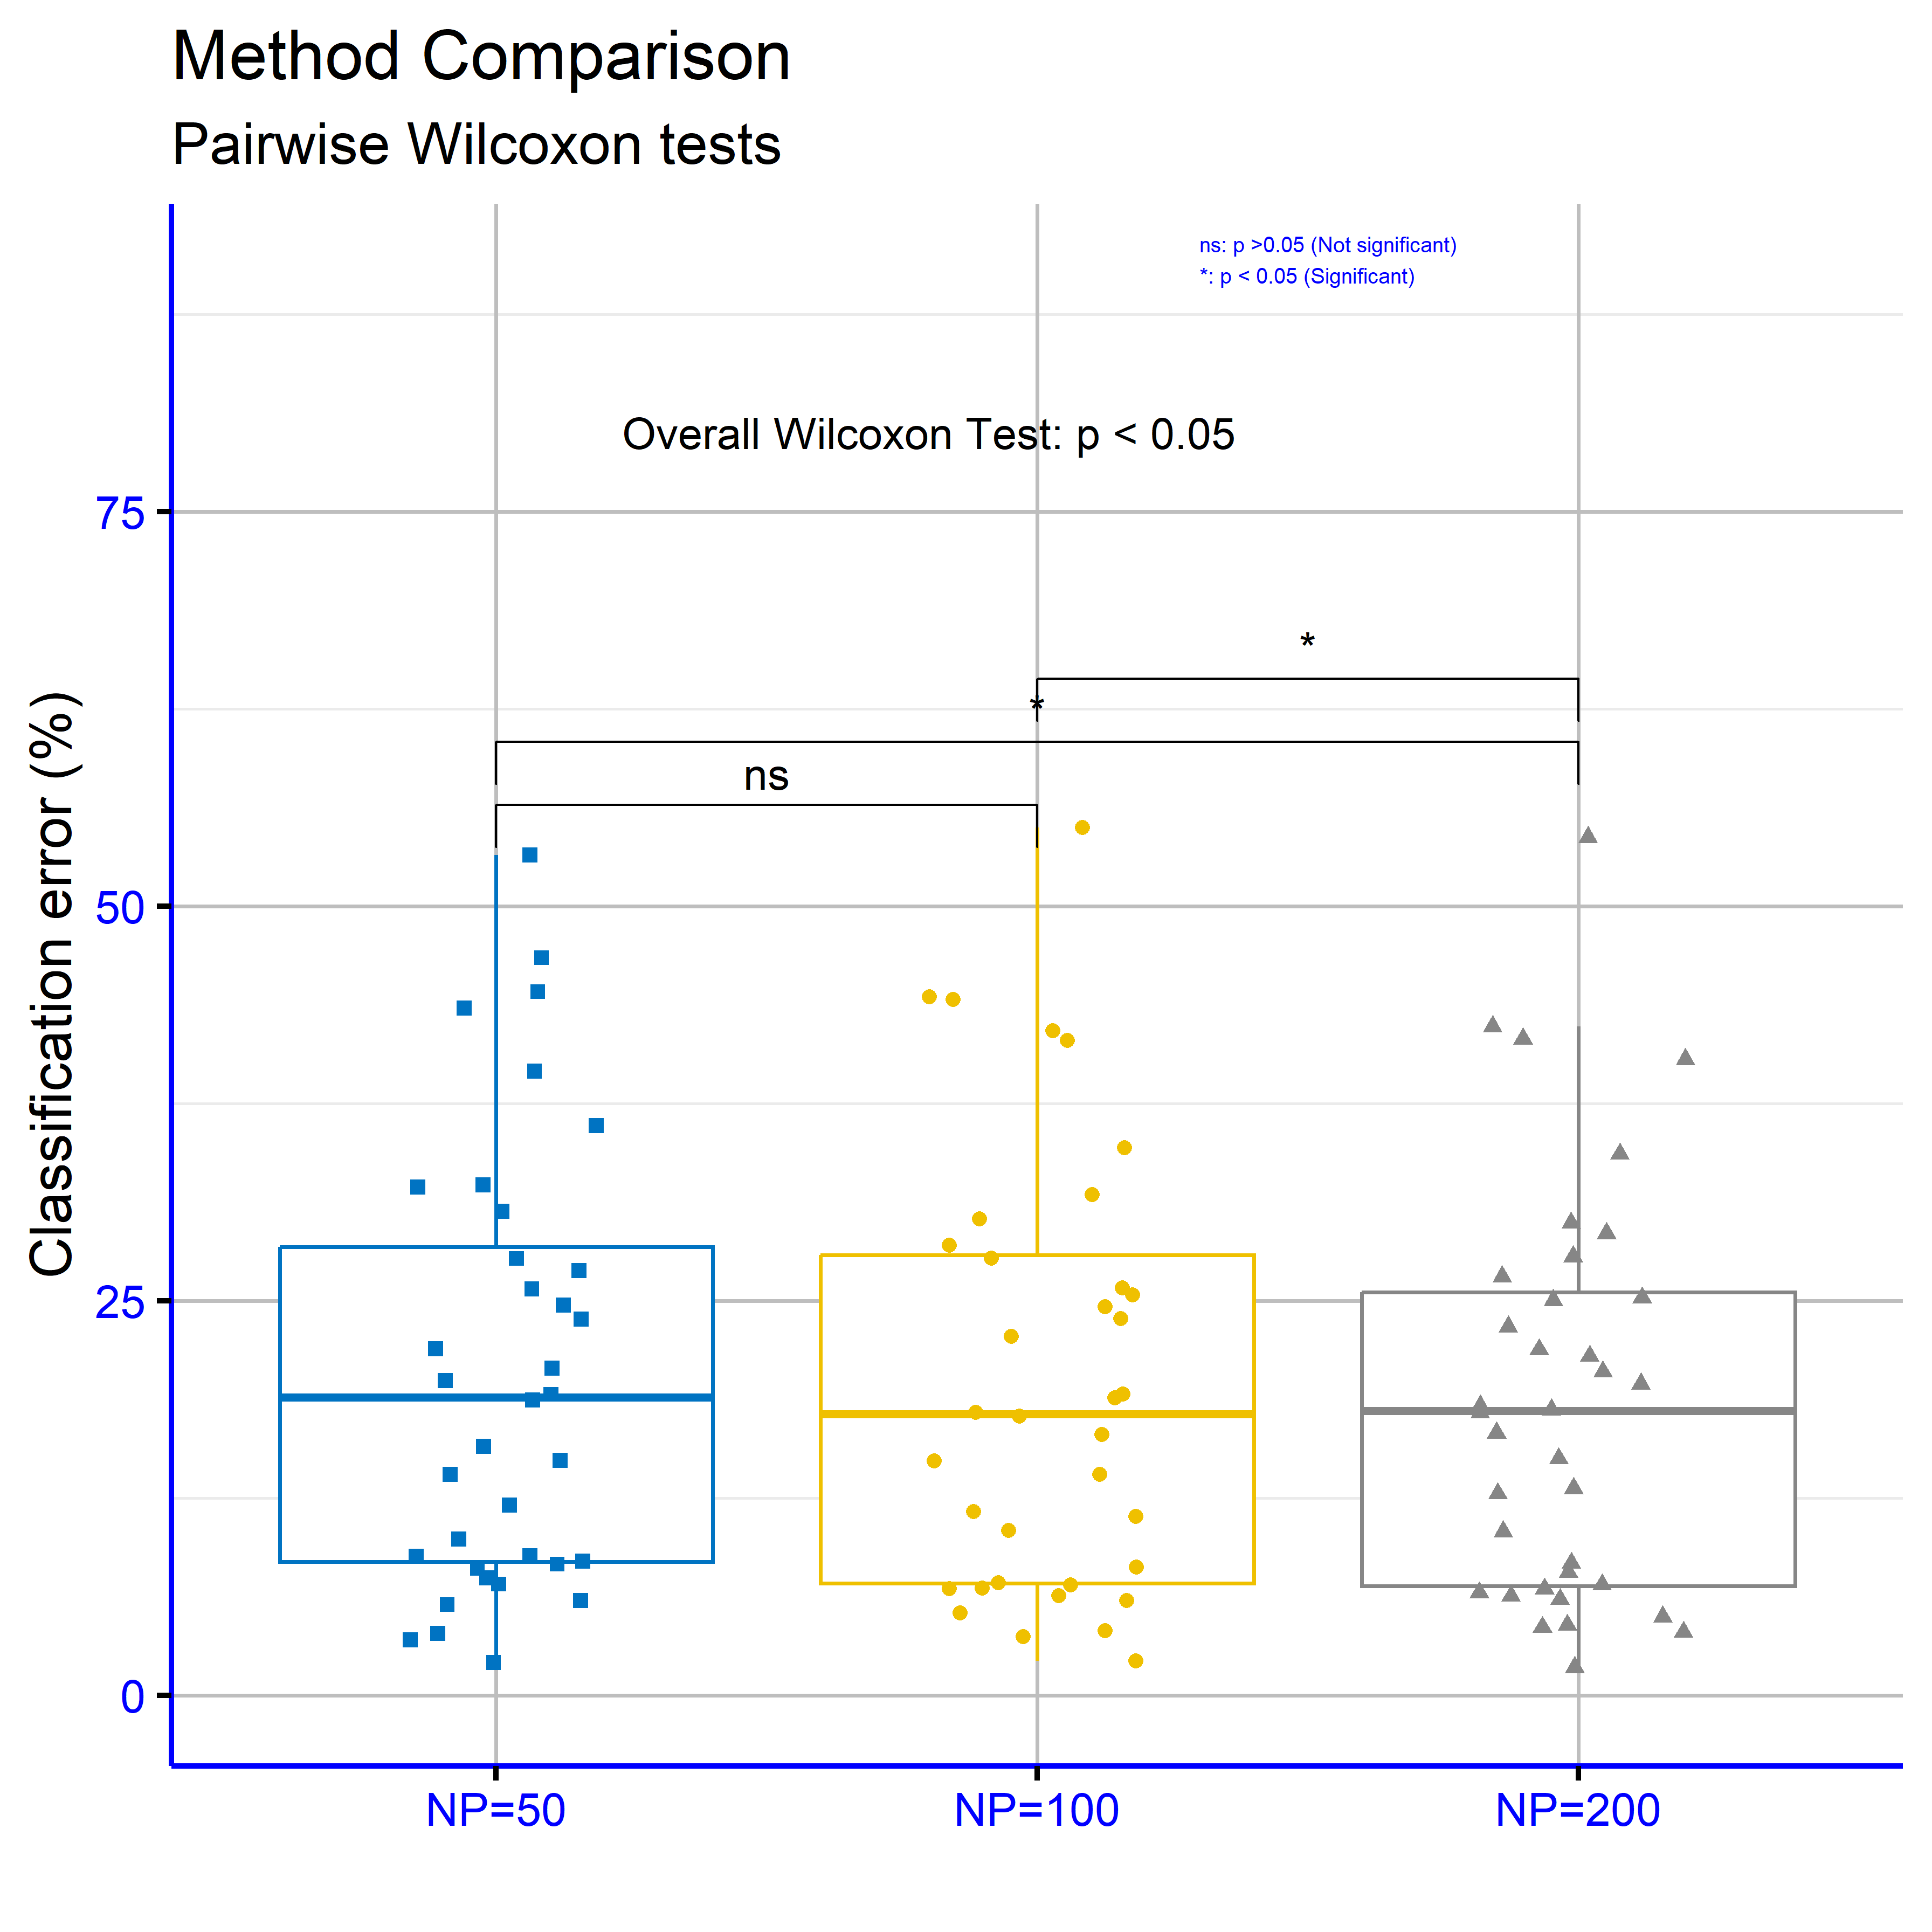
\includegraphics[scale=0.5]{img5}
\par\end{centering}
\caption{Statistical comparison for the experiments conducted on the classification
datasets using the proposed method and different values for the parameter
NP.\protect\label{fig:statNPClass}}

\end{figure}

Finally, Figure \ref{fig:statNPRegression} evaluates regression datasets
for different values of the critical parameter \textquotedbl NP\textquotedbl{}
within the proposed model. The respective p-values are: NP=50 vs NP=100:
p=0.08, NP=50 vs NP=200: p=0.012 and NP=100 vs NP=200: p=0.025. These
results show that the comparisons NP=50 vs NP=200 and NP=100 vs NP=200
exhibit statistically significant differences, while the comparison
NP=50 vs NP=100 does not.

\begin{figure}[H]
\begin{centering}
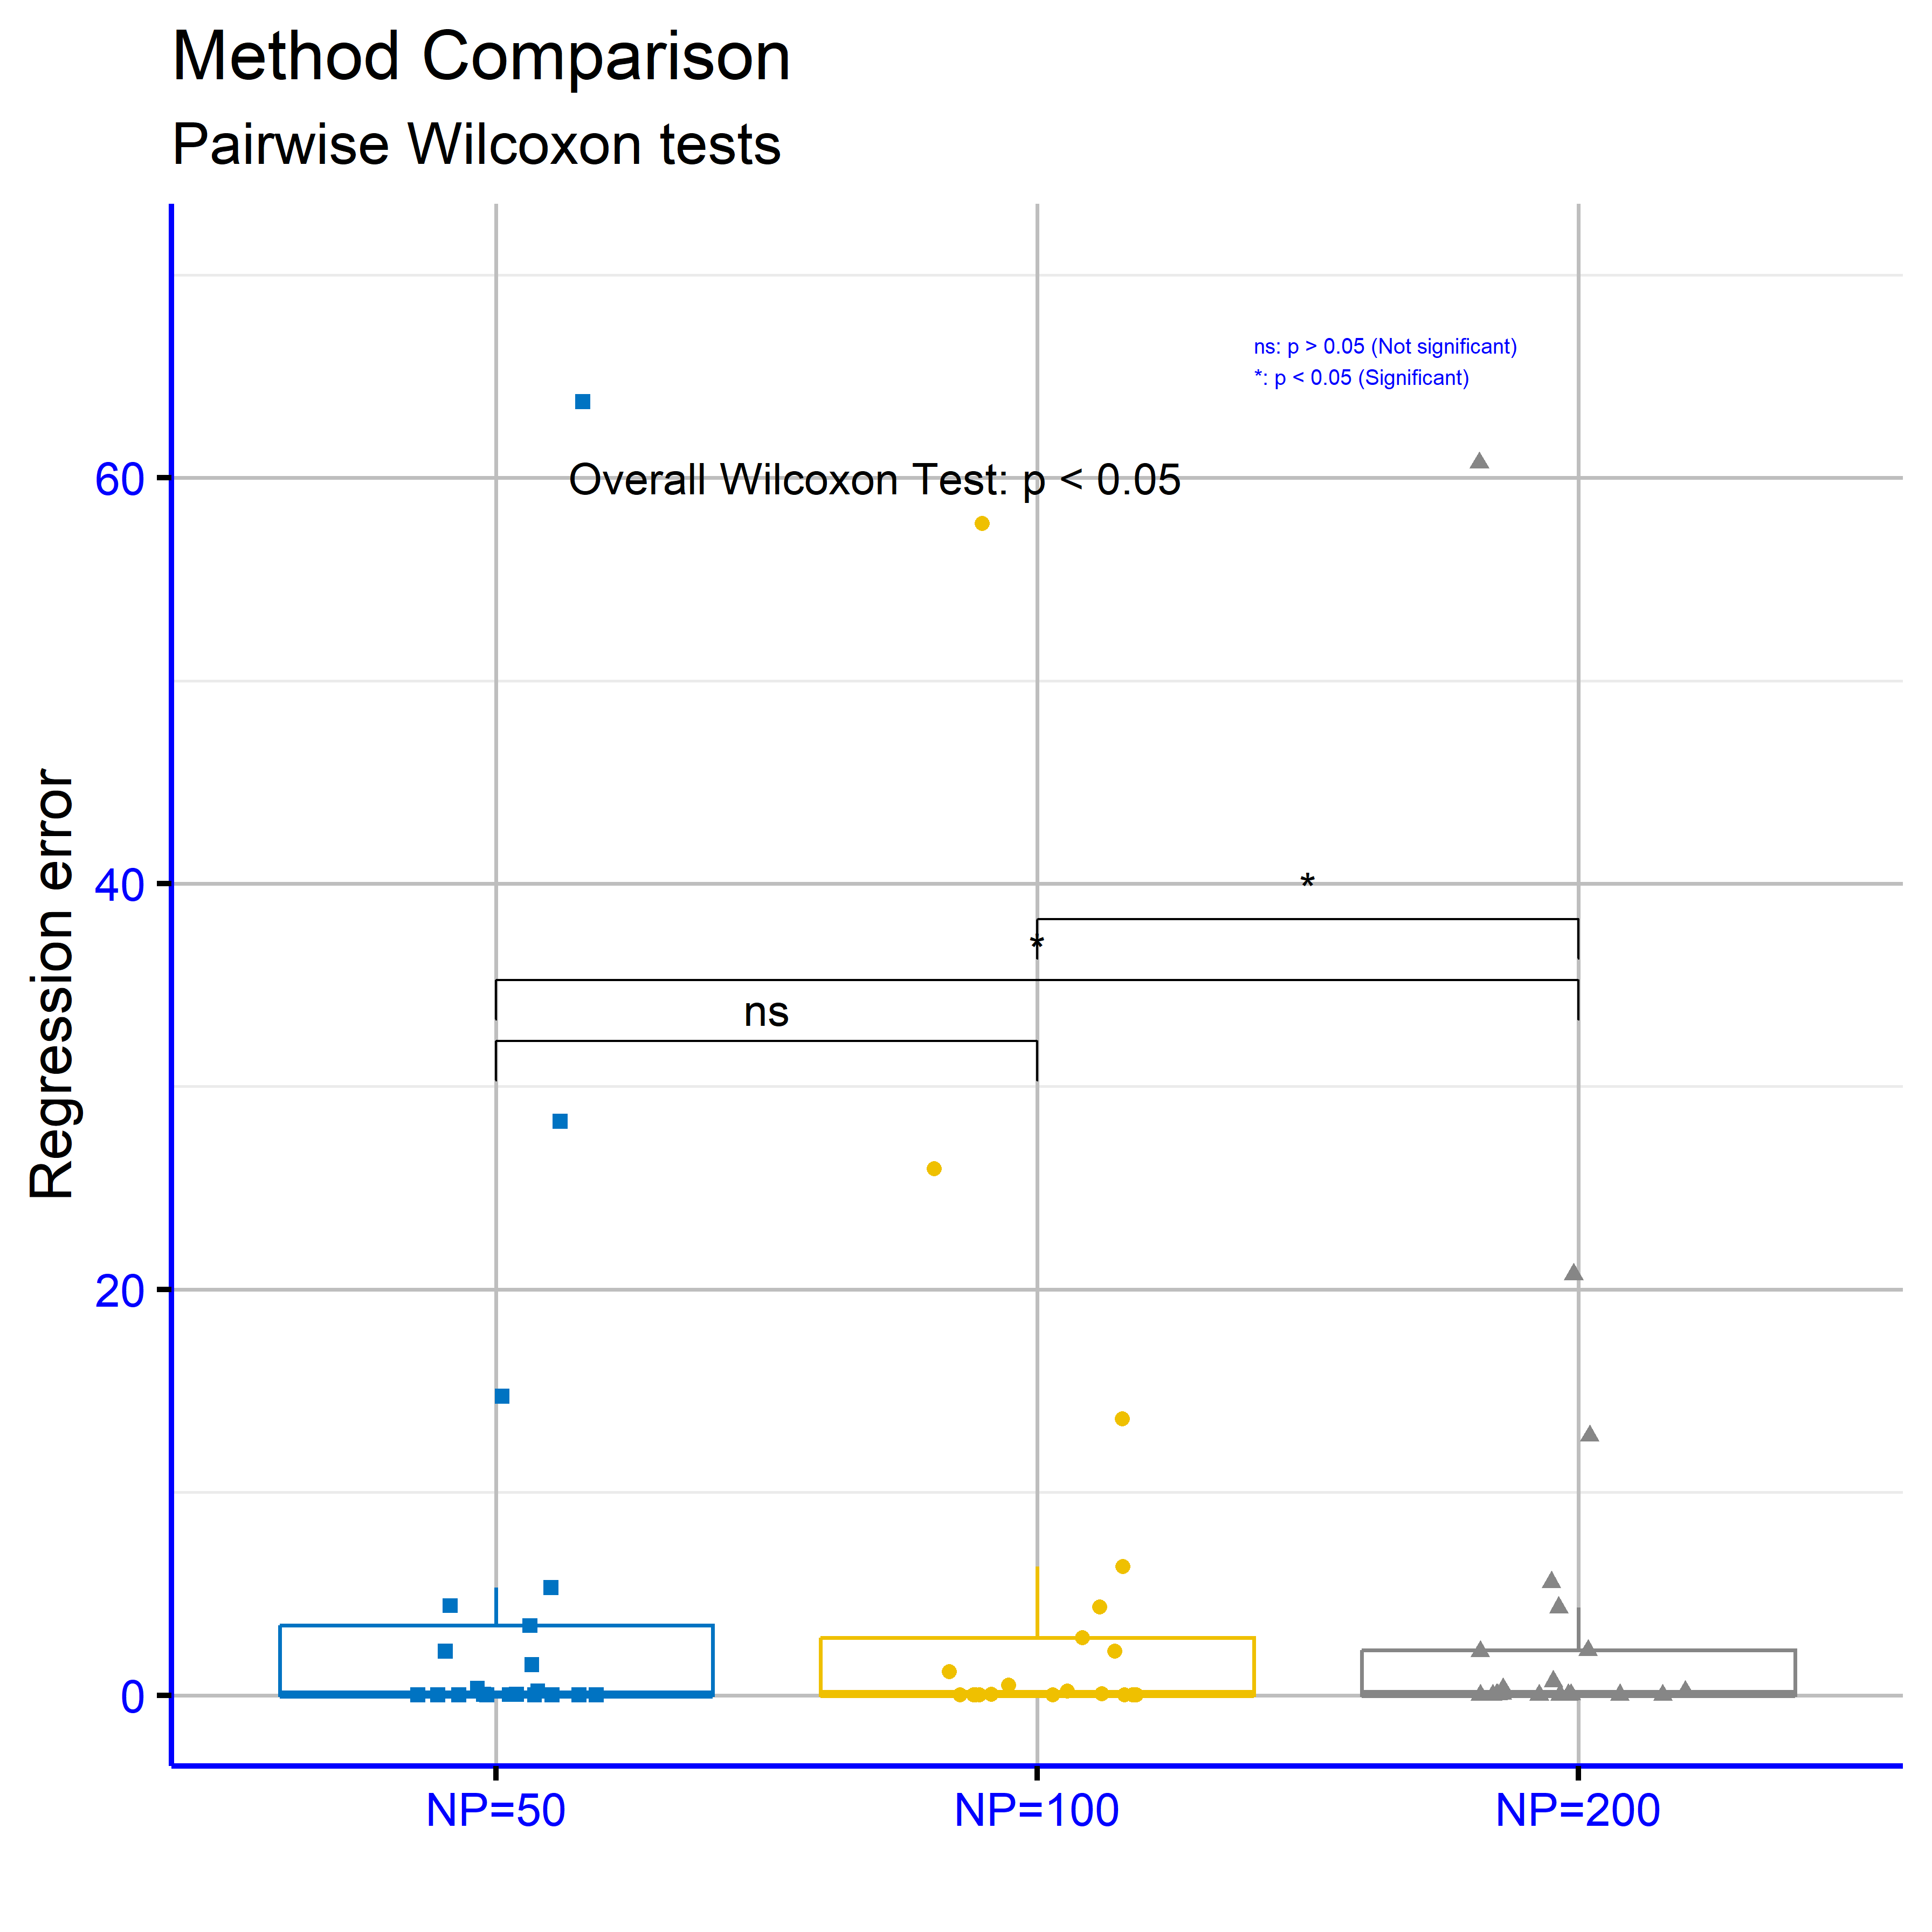
\includegraphics[scale=0.5]{img6}
\par\end{centering}
\caption{Statistical comparison for the conducted experiments on the regression
datasets using the proposed method and different values of the parameter
NP.\protect\label{fig:statNPRegression}}

\end{figure}


\subsection{Discussion}

This study introduces an innovative three-stage evolutionary method
for training artificial neural networks (ANNs), with the primary goal
of reducing both training error and overfitting. The results show
that the proposed approach achieves a mean classification error of
18.73\% and a mean regression error of 5.23, significantly outperforming
conventional methods such as ADAM, BFGS, PRUNE, genetic algorithms,
and radial basis function (RBF) networks. This improvement demonstrates
that combining genetic algorithms with differential evolution to define
optimal parameter bounds is an effective strategy for enhancing model
generalization. Specifically, the use of a modified fitness function,
which penalizes large deviations in weight values, appears to limit
the networks' tendency to overfit training data. For example, in datasets
like \textquotedbl DERMATOLOGY,\textquotedbl{} where the classification
error drops to 4.97\%, the method maintains high accuracy even in
cases of high variability.

Compared to previous studies that focused on standalone techniques
like genetic algorithm-based training or Adam optimizers, the current
method introduces two critical innovations. First, differential evolution
in the second stage enables systematic exploration of the parameter
space to identify optimal value intervals for weights. Second, the
multi-stage nature of the process initial boundary estimation, interval
optimization, and final training provides a structured framework for
managing problem complexity. These enhancements explain the significant
reduction in mean error compared to prior methods, such as the decrease
from 26.13\% to 18.73\% in classification and from 10.02 to 5.23 in
regression.

However, the method is not without limitations. A primary constraint
is its high computational cost, stemming from the three-stage process
and the large number of agents (NP=200) required to explore the parameter
space. Additionally, the method’s performance heavily depends on hyperparameter
tuning, such as crossover probability (CR). For instance, in datasets
like \textquotedbl SEGMENT\textquotedbl{} (27.80\% error) or \textquotedbl STOCK\textquotedbl{}
(5.57 error), the method shows relative weakness, likely due to data
complexity or noise. Furthermore, the use of a single hidden layer
(H=10) may be insufficient for high-dimensional problems, highlighting
the need for more complex architectures.

Error sources can be attributed to multiple factors. In medical datasets
like \textquotedbl CLEVELAND\textquotedbl{} (42.38\% error), noise
or class imbalance may affect accuracy. Additionally, random weight
initialization in the first stage can lead to suboptimal solutions,
while the network’s static architecture limits its ability to handle
non-linear relationships. However, a clear trend emerges: increasing
the number of agents (NP) improves performance, as seen in the reduction
of mean classification error from 20.36\% (NP=50) to 18.73\% (NP=200).
This suggests that broader parameter space exploration enhances generalization.

\section{Conclusions\protect\label{sec:Conclusions}}

The proposed evolutionary method, based on differential evolution,
proves highly effective in optimizing the weights of artificial neural
networks, significantly reducing both training error and overfitting.
Compared to other popular methods such as ADAM, BFGS, PRUNE genetic
algorithms, and radial basis function (RBF) networks, the new approach
demonstrates superior performance in classification tasks with a mean
error of 18.73\% and regression tasks with a mean error of 5.23\%.
Despite these positive results, certain datasets, such as \textquotedbl SEGMENT\textquotedbl{}
and \textquotedbl STOCK,\textquotedbl{} exhibit higher errors, likely
due to data complexity or inherent noise affecting prediction accuracy.
The random computation of parameter F and the use of a larger number
of agents (e.g., NP=200) enhance system performance. However, smaller
NP values yield better results in some cases, highlighting the need
for adaptive parameter tuning mechanisms during optimization.

The significance of this research lies in the method’s ability to
address two critical challenges in machine learning: reducing training
error and controlling overfitting. By sequentially using genetic algorithms
for initial boundary definition, differential evolution for interval
optimization, and a final training phase, the method provides a structured
framework that enhances model generalization. This makes it particularly
useful in applications where reliability and interpretability are
critical, such as medical diagnosis or industrial failure prediction.
For example, the exceptional performance on the \textquotedbl DERMATOLOGY\textquotedbl{}
dataset (4.97\% error) demonstrates its robustness even under high-variance
conditions.

However, the method operates within specific constraints. High computational
costs, due to the three-stage process and large number of agents,
limit its applicability in real-time or resource-constrained environments.
Additionally, its performance heavily depends on manual hyperparameter
tuning, such as crossover probability (CR). Furthermore, the use of
simple architectures with a single hidden layer (H=10) restricts its
ability to model complex relationships, as seen in underperformance
on datasets like \textquotedbl SEGMENT\textquotedbl{} (27.80\% error).
Noise in the data or class imbalance, as in \textquotedbl CLEVELAND\textquotedbl{}
(42.38\% error), can worsen results, emphasizing the need for preprocessing
or domain-specific adaptations.

For future research, developing mechanisms for dynamic parameter tuning
(e.g., automated selection of CR or NP) is essential to reduce reliance
on manual experimentation. Applying the method to high-dimensional
data, such as images or text, would evaluate its flexibility in domains
like computer vision or natural language processing. Combining it
with techniques like reinforcement learning or attention mechanisms
could improve adaptability in dynamic environments. Finally, a theoretical
analysis of the algorithm’s convergence and stability, alongside empirical
studies on underperforming datasets, could isolate error sources (e.g.,
noise sensitivity) and lead to optimizations.

In practical terms, the method is highly relevant in domains where
generalization and interpretability outweigh speed, such as healthcare
or critical infrastructure systems. However, its current weaknesses
necessitate cautious application in resource-limited or highly complex
scenarios. With strategic improvements in dynamic tuning and integration
with advanced architectures, the method could become a cornerstone
tool for next-generation neural networks, balancing theoretical innovation
and practical utility.

A key problem of the new technique is the slow training times of artificial
neural networks, since it is a three-stage technique. In each stage
a separate stochastic technique must be applied. This means that the
execution time will be increased compared to other techniques, such
as the simple genetic algorithm. Of course, some individual parts
of the process can be accelerated by using parallel computing techniques.
Finally, although the method uses a genetic algorithm in its last
stage to evaluate the parameter value ranges, other optimization techniques
can be used in its place, such as the Differential Evolution technique
and the PSO technique.

$ $

\authorcontributions{V.C. and I.G.T. conducted the experiments, employing several datasets
and provided the comparative experiments. D.T. and V.C. performed
the statistical analysis and prepared the manuscript. All authors
have read and agreed to the published version of the manuscript.}

\funding{This research received no external funding.}

\institutionalreview{Not applicable.}

\informedconsent{Not applicable.}

\dataavailability{Not applicable.}

\acknowledgments{This research has been financed by the European Union : Next Generation
EU through the Program Greece 2.0 National Recovery and Resilience
Plan , under the call RESEARCH -- CREATE -- INNOVATE, project name
“iCREW: Intelligent small craft simulator for advanced crew training
using Virtual Reality techniques\textquotedbl{} (project code:TAEDK-06195).}

\conflictsofinterest{The authors declare no conflicts of interest.}

\begin{adjustwidth}{-\extralength}{0cm}{}

\reftitle{References}
\begin{thebibliography}{999}
\bibitem{nn1}Abiodun, O. I., Jantan, A., Omolara, A. E., Dada, K.
V., Mohamed, N. A., \& Arshad, H. (2018). State-of-the-art in artificial
neural network applications: A survey. Heliyon, 4(11).

\bibitem{nn2}Suryadevara, S., \& Yanamala, A. K. Y. (2021). A Comprehensive
Overview of Artificial Neural Networks: Evolution, Architectures,
and Applications. Revista de Inteligencia Artificial en Medicina,
12(1), 51-76.

\bibitem{nn_image}M. Egmont-Petersen, D. de Ridder, H. Handels, Image
processing with neural networks---a review, Pattern Recognition \textbf{35},
pp. 2279-2301, 2002.

\bibitem{nn_timeseries}G.Peter Zhang, Time series forecasting using
a hybrid ARIMA and neural network model, Neurocomputing \textbf{50},
pp. 159-175, 2003.

\bibitem{nn_credit}Z. Huang, H. Chen, C.-Jung Hsu, W.-Hwa Chen, S.
Wu, Credit rating analysis with support vector machines and neural
networks: a market comparative study, Decision Support Systems \textbf{37},
pp. 543-558, 2004.

\bibitem{nnphysics1}P. Baldi, K. Cranmer, T. Faucett et al, Parameterized
neural networks for high-energy physics, Eur. Phys. J. C \textbf{76},
2016.

\bibitem{nnphysics2}Baldi, P., Cranmer, K., Faucett, T., Sadowski,
P., \& Whiteson, D. (2016). Parameterized neural networks for high-energy
physics. The European Physical Journal C, 76(5), 1-7.

\bibitem{nnastro}Firth, A. E., Lahav, O., \& Somerville, R. S. (2003).
Estimating photometric redshifts with artificial neural networks.
Monthly Notices of the Royal Astronomical Society, 339(4), 1195-1202.

\bibitem{nn_solar}A. Kumar Yadav, S.S. Chandel, Solar radiation prediction
using Artificial Neural Network techniques: A review, Renewable and
Sustainable Energy Reviews \textbf{33}, pp. 772-781, 2014.

\bibitem{nnagr2}A. Escamilla-García, G.M. Soto-Zarazúa, M. Toledano-Ayala,
E. Rivas-Araiza, A. Gastélum-Barrios, Abraham,Applications of Artificial
Neural Networks in Greenhouse Technology and Overview for Smart Agriculture
Development, Applied Sciences \textbf{10}, Article number 3835, 2020.

\bibitem{bpnn1}Vora, K., \& Yagnik, S. (2014). A survey on backpropagation
algorithms for feedforward neural networks. International Journal
of Engineering Development and Research, 1(3), 193-197.

\bibitem{rpropnn-1}Pajchrowski, T., Zawirski, K., \& Nowopolski,
K. (2014). Neural speed controller trained online by means of modified
RPROP algorithm. IEEE transactions on industrial informatics, 11(2),
560-568.

\bibitem{nn_adam}D. P. Kingma, J. L. Ba, ADAM: a method for stochastic
optimization, in: Proceedings of the 3rd International Conference
on Learning Representations (ICLR 2015), pp. 1--15, 2015.

\bibitem{nn_leve}Lera, G., \& Pinzolas, M. (2002). Neighborhood based
Levenberg-Marquardt algorithm for neural network training. IEEE transactions
on neural networks, 13(5), 1200-1203.

\bibitem{nn_siman}C.L. Kuo, E.E. Kuruoglu, W.K.V. Chan, Neural Network
Structure Optimization by Simulated Annealing, Entropy \textbf{24},
348, 2022.

\bibitem{geneticnn}Reynolds, J., Rezgui, Y., Kwan, A., \& Piriou,
S. (2018). A zone-level, building energy optimisation combining an
artificial neural network, a genetic algorithm, and model predictive
control. Energy, 151, 729-739.

\bibitem{psonn}Das, G., Pattnaik, P. K., \& Padhy, S. K. (2014).
Artificial neural network trained by particle swarm optimization for
non-linear channel equalization. Expert Systems with Applications,
41(7), 3491-3496.

\bibitem{aco_nn}K.M. Salama, A.M. Abdelbar, Learning neural network
structures with ant colony algorithms, Swarm Intell \textbf{9}, pp.
229--265, 2015.

\bibitem{gwo_nn}S. Mirjalili, How effective is the Grey Wolf optimizer
in training multi-layer perceptrons, Appl Intell \textbf{43}, pp.
150--161, 2015.

\bibitem{whale_nn}I. Aljarah, H. Faris, S. Mirjalili, Optimizing
connection weights in neural networks using the whale optimization
algorithm, Soft Comput \textbf{22}, pp. 1--15, 2018. 

\bibitem{tabunn}R.S. Sexton, B. Alidaee, R.E. Dorsey, J.D. Johnson,
Global optimization for artificial neural networks: A tabu search
application. European Journal of Operational Research \textbf{106},
pp. 570-584, 1998.

\bibitem{nn_hybrid}J.-R. Zhang, J. Zhang, T.-M. Lok, M.R. Lyu, A
hybrid particle swarm optimization--back-propagation algorithm for
feedforward neural network training, Applied Mathematics and Computation
\textbf{185}, pp. 1026-1037, 2007.

\bibitem{nn_cascade}G. Zhao, T. Wang, Y. Jin, C. Lang, Y. Li, H.
Ling, The Cascaded Forward algorithm for neural network training,
Pattern Recognition \textbf{161}, 111292, 2025.

\bibitem{nn_gpu1}K-Su Oh, K. Jung, GPU implementation of neural networks,
Pattern Recognition \textbf{37}, pp. 1311-1314, 2004.

\bibitem{nn_gpu2}M. Zhang, K. Hibi, J. Inoue, GPU-accelerated artificial
neural network potential for molecular dynamics simulation, Computer
Physics Communications \textbf{285}, 108655, 2023. 

\bibitem{nnsharing1}S.J. Nowlan and G.E. Hinton, Simplifying neural
networks by soft weight sharing, Neural Computation 4, pp. 473-493,
1992.

\bibitem{nnprunning1}S.J. Hanson and L.Y. Pratt, Comparing biases
for minimal network construction with back propagation, In D.S. Touretzky
(Ed.), Advances in Neural Information Processing Systems, Volume 1,
pp. 177-185, San Mateo, CA: Morgan Kaufmann, 1989.

\bibitem{nnearly1}Lutz Prechelt, Automatic early stopping using cross
validation: quantifying the criteria, Neural Networks \textbf{11},
pp. 761-767, 1998.

\bibitem{nndecay1}N. K. Treadgold and T. D. Gedeon, Simulated annealing
and weight decay in adaptive learning: the SARPROP algorithm,IEEE
Transactions on Neural Networks \textbf{9}, pp. 662-668, 1998.

\bibitem[(2014)]{Dropout}Nitish Srivastava, G E Hinton, Alex Krizhevsky,
Ilya Sutskever, Ruslan R Salakhutdinov, Dropout: a simple way to prevent
neural networks from overfitting, Journal of Machine Learning Research
\textbf{15}, pp. 1929-1958, 2014.

\bibitem[(2014)]{Sarprop}N.K. Treadgold, T.D. Gedeon, Simulated annealing
and weight decay in adaptive learning: the SARPROP algorithm, IEEE
Trans. on Neural Networks 9, pp. 662-668, 1998.

\bibitem[(2014)]{nnpos}M.D. Shahjahan, M. Kazuyuki, Neural network
training algorithm with possitive correlation, IEEE Trans. Inf \&
Syst. \textbf{88}, pp. 2399-2409, 2005.

\bibitem{nn_arch1}J. Arifovic, R. Gençay, Using genetic algorithms
to select architecture of a feedforward artificial neural network,
Physica A: Statistical Mechanics and its Applications \textbf{289},
pp. 574-594, 2001.

\bibitem{nn_arch2}P.G. Benardos, G.C. Vosniakos, Optimizing feedforward
artificial neural network architecture, Engineering Applications of
Artificial Intelligence \textbf{20}, pp. 365-382, 2007.

\bibitem{nn_arch3}B.A. Garro, R.A. Vázquez, Designing Artificial
Neural Networks Using Particle Swarm Optimization Algorithms, Computational
Intelligence and Neuroscience, 369298, 2015. 

\bibitem[(2014)]{nn_arch4}B. Baker, O. Gupta, N. Naik, R. Raskar,
Designing neural network architectures using reinforcement learning.
arXiv preprint arXiv:1611.02167, 2016.

\bibitem{nn_arch5}M. M. Islam, M. A. Sattar, M. F. Amin, X. Yao,
K. Murase, A New Adaptive Merging and Growing Algorithm for Designing
Artificial Neural Networks, IEEE Transactions on Systems, Man, and
Cybernetics, Part B (Cybernetics) \textbf{39}, pp. 705-722, 2009. 

\bibitem[(2014)]{ge1}M. O’Neill, C. Ryan, Grammatical evolution,
IEEE Trans. Evol. Comput. \textbf{5,}pp. 349--358, 2001.

\bibitem[(2014)]{nnc}I.G. Tsoulos, D. Gavrilis, E. Glavas, Neural
network construction and training using grammatical evolution, Neurocomputing
\textbf{72}, pp. 269-277, 2008.

\bibitem[(2014)]{nn_number_neurons}Liu, Y., Starzyk, J. A., \& Zhu,
Z. (2007). Optimizing number of hidden neurons in neural networks.
EeC, 1(1), 6.

\bibitem[(2014)]{nn_over_runoff}A.P. Piotrowski, J.J. Napiorkowski,
A comparison of methods to avoid overfitting in neural networks training
in the case of catchment runoff modelling, Journal of Hydrology \textbf{476},
pp 97-111, 2013.

\bibitem[(2014)]{nn_overfitting_review}Ying, X. (2019, February).
An overview of overfitting and its solutions. In Journal of physics:
Conference series (Vol. 1168, p. 022022). IOP Publishing.

\bibitem{gen_review}Lambora, A., Gupta, K., \& Chopra, K. (2019,
February). Genetic algorithm-A literature review. In 2019 international
conference on machine learning, big data, cloud and parallel computing
(COMITCon) (pp. 380-384). IEEE.

\bibitem{de_review}Pant, M., Zaheer, H., Garcia-Hernandez, L., \&
Abraham, A. (2020). Differential Evolution: A review of more than
two decades of research. Engineering Applications of Artificial Intelligence,
90, 103479.

\bibitem{de_symmetry1}Y.H. Li, J.Q. Wang, X.J. Wang, Y.L. Zhao, X.H.
Lu, D.L. Liu, Community Detection Based on Differential Evolution
Using Social Spider Optimization, Symmetry \textbf{9}, 2017.

\bibitem{de_symmetry3}W. Yang, E.M. Dilanga Siriwardane, R. Dong,
Y. Li, J. Hu, Crystal structure prediction of materials with high
symmetry using differential evolution, J. Phys.: Condens. Matter \textbf{33}
455902, 2021.

\bibitem{de_symmetry6}C.Y. Lee, C.H. Hung, Feature Ranking and Differential
Evolution for Feature Selection in Brushless DC Motor Fault Diagnosis
, Symmetry \textbf{13}, 2021.

\bibitem{de_symmetry7}S. Saha, R. Das, Exploring differential evolution
and particle swarm optimization to develop some symmetry-based automatic
clustering techniques: application to gene clustering, Neural Comput
\& Applic \textbf{30}, pp. 735--757, 2018.

\bibitem[(2014)]{ga_nn1}J. Arifovic, R. Gençay, Using genetic algorithms
to select architecture of a feedforward artificial neural network,
Physica A: Statistical Mechanics and its Applications \textbf{289},
pp. 574-594, 2001. 

\bibitem[(2014)]{ga_nn2}F. H. F. Leung, H. K. Lam, S. H. Ling, P.
K. S. Tam, Tuning of the structure and parameters of a neural network
using an improved genetic algorithm, IEEE Transactions on Neural Networks
\textbf{14}, pp. 79-88, 2003.

\bibitem[(2014)]{ga_nn3}F. Ahmadizar, K. Soltanian, F. AkhlaghianTab,
I. Tsoulos, Artificial neural network development by means of a novel
combination of grammatical evolution and genetic algorithm, Engineering
Applications of Artificial Intelligence \textbf{39}, pp. 1-13, 2015. 

\bibitem{Hornik}Hornik, K., Stinchcombe, M., \& White, H. (1989).
Multilayer feedforward networks are universal approximators. Neural
networks, 2(5), 359-366.

\bibitem{kaelo}P. Kaelo, M.M. Ali, Integrated crossover rules in
real coded genetic algorithms, European Journal of Operational Research
\textbf{176}, pp. 60-76, 2007.

\bibitem[(1989)]{uci} M. Kelly, R. Longjohn, K. Nottingham, The UCI
Machine Learning Repository, https://archive.ics.uci.edu.

\bibitem{Keel}J. Alcalá-Fdez, A. Fernandez, J. Luengo, J. Derrac,
S. García, L. Sánchez, F. Herrera. KEEL Data-Mining Software Tool:
Data Set Repository, Integration of Algorithms and Experimental Analysis
Framework. Journal of Multiple-Valued Logic and Soft Computing 17,
pp. 255-287, 2011.

\bibitem{appendicitis}Weiss, Sholom M. and Kulikowski, Casimir A.,
Computer Systems That Learn: Classification and Prediction Methods
from Statistics, Neural Nets, Machine Learning, and Expert Systems,
Morgan Kaufmann Publishers Inc, 1991.

\bibitem[Tzimourta(2018)]{alcohol}Tzimourta, K.D.; Tsoulos, I.; Bilero,
I.T.; Tzallas, A.T.; Tsipouras, M.G.; Giannakeas, N. Direct Assessment
of Alcohol Consumption in Mental State Using Brain Computer Interfaces
and Grammatical Evolution. Inventions 2018, 3, 51.

\bibitem[Quinlan(2018)]{australian}J.R. Quinlan, Simplifying Decision
Trees. International Journal of Man-Machine Studies \textbf{27}, pp.
221-234, 1987. 

\bibitem{balance}T. Shultz, D. Mareschal, W. Schmidt, Modeling Cognitive
Development on Balance Scale Phenomena, Machine Learning \textbf{16},
pp. 59-88, 1994.

\bibitem[(2004)]{cleveland1}Z.H. Zhou,Y. Jiang, NeC4.5: neural ensemble
based C4.5,\textquotedbl{} in IEEE Transactions on Knowledge and Data
Engineering \textbf{16}, pp. 770-773, 2004.

\bibitem[(1998)]{dermatology}G. Demiroz, H.A. Govenir, N. Ilter,
Learning Differential Diagnosis of Eryhemato-Squamous Diseases using
Voting Feature Intervals, Artificial Intelligence in Medicine. \textbf{13},
pp. 147--165, 1998.

\bibitem[(1996)]{ecoli}P. Horton, K.Nakai, A Probabilistic Classification
System for Predicting the Cellular Localization Sites of Proteins,
In: Proceedings of International Conference on Intelligent Systems
for Molecular Biology \textbf{4}, pp. 109-15, 1996.

\bibitem[(1977)]{hayes-roth}B. Hayes-Roth, B., F. Hayes-Roth. Concept
learning and the recognition and classification of exemplars. Journal
of Verbal Learning and Verbal Behavior \textbf{16}, pp. 321-338, 1977.

\bibitem[(1997)]{heart}I. Kononenko, E. Šimec, M. Robnik-Šikonja,
Overcoming the Myopia of Inductive Learning Algorithms with RELIEFF,
Applied Intelligence \textbf{7}, pp. 39--55, 1997

\bibitem[(2002)]{housevotes}R.M. French, N. Chater, Using noise to
compute error surfaces in connectionist networks: a novel means of
reducing catastrophic forgetting, Neural Comput. \textbf{14}, pp.
1755-1769, 2002.

\bibitem[(2004)]{ion1}J.G. Dy , C.E. Brodley, Feature Selection for
Unsupervised Learning, The Journal of Machine Learning Research \textbf{5},
pp 845--889, 2004.

\bibitem[(2002)]{liver} J. Garcke, M. Griebel, Classification with
sparse grids using simplicial basis functions, Intell. Data Anal.
\textbf{6}, pp. 483-502, 2002.

\bibitem[(2002)]{lymography}G. Cestnik, I. Konenenko, I. Bratko,
Assistant-86: A Knowledge-Elicitation Tool for Sophisticated Users.
In: Bratko, I. and Lavrac, N., Eds., Progress in Machine Learning,
Sigma Press, Wilmslow, pp. 31-45, 1987. 

\bibitem[(2007)]{mammographic}M. Elter, R. Schulz-Wendtland, T. Wittenberg,
The prediction of breast cancer biopsy outcomes using two CAD approaches
that both emphasize an intelligible decision process, Med Phys. \textbf{34},
pp. 4164-72, 2007.

\bibitem[(2007)]{parkinsons1}M.A. Little, P.E. McSharry, S.J Roberts
et al, Exploiting Nonlinear Recurrence and Fractal Scaling Properties
for Voice Disorder Detection. BioMed Eng OnLine \textbf{6}, 23, 2007.

\bibitem[(2007)]{pima}J.W. Smith, J.E. Everhart, W.C. Dickson, W.C.
Knowler, R.S. Johannes, Using the ADAP learning algorithm to forecast
the onset of diabetes mellitus, In: Proceedings of the Symposium on
Computer Applications and Medical Care IEEE Computer Society Press,
pp.261-265, 1988.

\bibitem[(2007)]{popfailures}D.D. Lucas, R. Klein, J. Tannahill,
D. Ivanova, S. Brandon, D. Domyancic, Y. Zhang, Failure analysis of
parameter-induced simulation crashes in climate models, Geoscientific
Model Development \textbf{6}, pp. 1157-1171, 2013.

\bibitem[(2007)]{regions2}N. Giannakeas, M.G. Tsipouras, A.T. Tzallas,
K. Kyriakidi, Z.E. Tsianou, P. Manousou, A. Hall, E.C. Karvounis,
V. Tsianos, E. Tsianos, A clustering based method for collagen proportional
area extraction in liver biopsy images (2015) Proceedings of the Annual
International Conference of the IEEE Engineering in Medicine and Biology
Society, EMBS, 2015-November, art. no. 7319047, pp. 3097-3100. 

\bibitem[(2007)]{saheart}T. Hastie, R. Tibshirani, Non-parametric
logistic and proportional odds regression, JRSS-C (Applied Statistics)
\textbf{36}, pp. 260--276, 1987.

\bibitem{segment}M. Dash, H. Liu, P. Scheuermann, K. L. Tan, Fast
hierarchical clustering and its validation, Data \& Knowledge Engineering
\textbf{44}, pp 109--138, 2003.

\bibitem[(2007)]{student}P. Cortez, A. M. Gonçalves Silva, Using
data mining to predict secondary school student performance, In Proceedings
of 5th FUture BUsiness TEChnology Conference (FUBUTEC 2008) (pp. 5--12).
EUROSIS-ETI, 2008.

\bibitem[(2007)]{transfusion}I-Cheng Yeh, King-Jang Yang, Tao-Ming
Ting, Knowledge discovery on RFM model using Bernoulli sequence, Expert
Systems with Applications \textbf{36}, pp. 5866-5871, 2009.

\bibitem[(2007)]{wdbc1}Jeyasingh, S., \& Veluchamy, M. (2017). Modified
bat algorithm for feature selection with the wisconsin diagnosis breast
cancer (WDBC) dataset. Asian Pacific journal of cancer prevention:
APJCP, 18(5), 1257.

\bibitem[(2007)]{wine1}M. Raymer, T.E. Doom, L.A. Kuhn, W.F. Punch,
Knowledge discovery in medical and biological datasets using a hybrid
Bayes classifier/evolutionary algorithm. IEEE transactions on systems,
man, and cybernetics. Part B, Cybernetics : a publication of the IEEE
Systems, Man, and Cybernetics Society, \textbf{33} , pp. 802-813,
2003.

\bibitem[(2007)]{eeg1}R. G. Andrzejak, K. Lehnertz, F.Mormann, C.
Rieke, P. David, and C. E. Elger, “Indications of nonlinear deterministic
and finite-dimensional structures in time series of brain electrical
activity: dependence on recording region and brain state,” Physical
Review E, vol. 64, no. 6, Article ID 061907, 8 pages, 2001. 

\bibitem[(2007)]{zoo}M. Koivisto, K. Sood, Exact Bayesian Structure
Discovery in Bayesian Networks, The Journal of Machine Learning Research\textbf{
5}, pp. 549--573, 2004.

\bibitem[(2007)]{abalone}Nash, W.J.; Sellers, T.L.; Talbot, S.R.;
Cawthor, A.J.; Ford, W.B. The Population Biology of Abalone (\_Haliotis\_
species) in Tasmania. I. Blacklip Abalone (\_H. rubra\_) from the
North Coast and Islands of Bass Strait, Sea Fisheries Division; Technical
Report No. 48; Department of Primary Industry and Fisheries, Tasmania:
Hobart, Australia, 1994; ISSN 1034-3288

\bibitem[(2007)]{airfoil}Brooks, T.F.; Pope, D.S.; Marcolini, A.M.
Airfoil Self-Noise and Prediction. Technical Report, NASA RP-1218.
July 1989. Available online: https://ntrs.nasa.gov/citations/19890016302
(accessed on 14 November 2024).

\bibitem[(2007)]{concrete}I.Cheng Yeh, Modeling of strength of high
performance concrete using artificial neural networks, Cement and
Concrete Research. \textbf{28}, pp. 1797-1808, 1998. 

\bibitem{friedman}Friedman, J. (1991): Multivariate Adaptative Regression
Splines. Annals of Statistics, 19:1, 1-{}-141. 

\bibitem[(2007)]{housing}D. Harrison and D.L. Rubinfeld, Hedonic
prices and the demand for clean ai, J. Environ. Economics \& Management
\textbf{5}, pp. 81-102, 1978.

\bibitem[(1994)]{momentum}Phansalkar, V. V., \& Sastry, P. S. (1994).
Analysis of the back-propagation algorithm with momentum. IEEE Transactions
on Neural Networks, 5(3), 505-506.

\bibitem[(2019)]{rmsprop}Zou, F., Shen, L., Jie, Z., Zhang, W., \&
Liu, W. (2019). A sufficient condition for convergences of adam and
rmsprop. In Proceedings of the IEEE/CVF Conference on computer vision
and pattern recognition (pp. 11127-11135).

\bibitem{powell}M.J.D Powell, A Tolerant Algorithm for Linearly Constrained
Optimization Calculations, Mathematical Programming \textbf{45}, pp.
547-566, 1989. 

\bibitem{neat}K. O. Stanley, R. Miikkulainen, Evolving Neural Networks
through Augmenting Topologies, Evolutionary Computation \textbf{10},
pp. 99-127, 2002.

\bibitem[(1991)]{rbf1}J. Park and I. W. Sandberg, Universal Approximation
Using Radial-Basis-Function Networks, Neural Computation \textbf{3},
pp. 246-257, 1991.

\bibitem[(2019)]{prune}Zhu, V., Lu, Y., \& Li, Q. (2006). MW-OBS:
An improved pruning method for topology design of neural networks.
Tsinghua Science and Technology, 11(4), 307-312.

\bibitem{fcn}Grzegorz Klima, Fast Compressed Neural Networks, available
from \url{http://fcnn.sourceforge.net/}.

\bibitem{de_migrant}J. Cheng, G. Zhang, F. Neri, Enhancing distributed
differential evolution with multicultural migration for global numerical
optimization. Information Sciences \textbf{247}, pp. 72-93, 2013.

\bibitem{de_adaptive}Wu, K., Liu, Z., Ma, N., \& Wang, D. (2022).
A Dynamic Adaptive Weighted Differential Evolutionary Algorithm. Computational
Intelligence and Neuroscience, 2022(1), 1318044.

\end{thebibliography}

\end{adjustwidth}{}
\end{document}
